\documentclass{ufpatcc}

\include{include}
%% Packages used for the TCC

%\usepackage{booktabs}

%%%% Definitions and New commnads %%%%

\newcommand{\sen}{\operatorname{sen}}
\newcommand{\mbeq}{\overset{!}{=}}

\renewcommand\Re{\operatorname{Re}}
\renewcommand\Im{\operatorname{Im}}

%%%% New control sequences %%%%

\newcommand{\redeq}[1] {\textcolor{red}{#1}}
\newcommand{\blueeq}[1] {\textcolor{blue}{#1}}
\newcommand{\att}[1] {\textcolor{red}{#1}}
% Used Packages:
\usepackage{tikz}
\usepackage{float}
\usepackage{steinmetz}
\usetikzlibrary{arrows,shapes,shapes.multipart}
%\usepackage[brazil]{babel}
\usepackage[T1]{fontenc}
\usepackage[utf8]{inputenc}
\usepackage{amsmath}
\usepackage{amsfonts}
\usepackage{enumitem} % To adjust lists
\usepackage{verbatim} % Multi-line comments
\usepackage{mathabx} % Package that contains the circular convolution symbol
\usepackage{graphicx}
\usepackage{caption}
\usepackage{subcaption}
\usepackage{units}
\usepackage{adjustbox}
\usepackage{dirtytalk}

%\usepackage[backend=bibtex8]{biblatex}

\ifpdf

\ifdefined\hyperref
\else
\usepackage[pdftex,colorlinks]{hyperref}
\fi

\hypersetup{%
pdftitle={Some title},
pdfauthor={Your name - LaPS - UFPA},
pdfkeywords={DSP,Signal},
pdfstartview={FitH}, %% <--
urlcolor=black,
%linkcolor=blue,
linkcolor=black,
%citecolor=red,
citecolor=black,
}

% Ensiar o Latex a separar silabas
\hyphenation{DMT En-ge-nhei-ro}


\ufpaTitulo{An FPGA-Based Radion Frontend for LTE Transmission on Cloud RAN}

\ufpaAutor{Gabriel Peixoto de Carvalho}
\ufpaSegundoAutor{}
\ufpaOrientador{Prof. Aldebaro Barreto da Rocha Klautau Junior}
\ufpaCoordenadorCurso{Prof. Jos\'{e} Augusto de Lima Barreiros}

\ufpaCoOrientador{Prof. Wilson Pacheco Ferreira}
\ufpaMembroBancaA{Prof. Francisco Carlos Bentes Frey Muller}
\ufpaMembroBancaB{Eng. Igor Mesquita de Almeida}


\begin{document}

\ufpaPaginaDeRosto

\ufpaPagRostodo

\ufpaPaginaDeAprovacao

%%%%%%%%%%%%%%%%%%%%
%   Oferecimento   %
%%%%%%%%%%%%%%%%%%%%

\begin{ufpaOferecimento}
\index{Oferecimento@Oferecimento}%
\addcontentsline{toc}{chapter}{Dedicat�ria}

\end{ufpaOferecimento}

%%%%%%%%%%%%%%%%%%%%
%  Agradecimento   %
%%%%%%%%%%%%%%%%%%%%

\begin{ufpaAgradecimentos}
\index{Agradecimentos@Agradecimentos}
\addcontentsline{toc}{chapter}{Agradecimentos}

\begin{flushright}
Gabriel Peixoto de Carvalho
\end{flushright}

\end{ufpaAgradecimentos}

%%%%%%%%%%%%%%%%%%%%
%      Ep�grafe     %
%%%%%%%%%%%%%%%%%%%%

\begin{ufpaEpigrafe}
Viva como se voc� fosse morrer amanh�. Aprenda como se voc� fosse viver para sempre.\\
\begin{flushright}Mahatma Gandhi\end{flushright}
\end{ufpaEpigrafe}

%%%%%%%%%%%%%%%%%%%%%
%  Lista de Siglas  %
%%%%%%%%%%%%%%%%%%%%%

\chapter*{Lista de Siglas} \label{sec:siglas}
\begin{enumerate}
 \item ADSL - \textit{Linha de assinante digital assim�trica}
 %\item AWGN - \textit{Ru�do aditivo branco Gaussiano}
 %\item BER - \textit{Taxa de erro de bit}
 %\item DFT - \textit{Transformada de Fourier discreta}
 %\item DMT - \textit{Multi-tom discreto}
 %\item DSL - \textit{Linha de assinante digital}
 %\item FEQ - \textit{Equalizador em frequ�ncia}
 %\item FFT - \textit{Transformada rápida de Fourier}
 %\item FTTH - \textit{Fibra até a residência}
 %\item G.fast - \textit{Acesso rápido aos terminais do assinante}
 %\item ICI - \textit{Interferência inter-portadora}
 %\item IDFT - \textit{Transformada de Fourier discreta inversa}
 %\item IFFT - \textit{Transformada rápida de Fourier inversa}
 %\item ISI - \textit{Interferência inter-simbólica}
 %\item OFDM - \textit{Modulação por divisão ortogonal de frequência}
 %\item PC - \textit{Prefixo cíclico}
 %\item PSD - \textit{Densidade espectral de potência}
 %\item RIC - \textit{Resposta impulsiva do canal}
 %\item SC - \textit{Sufixo cíclico}
 %\item SER - \textit{Taxa de erro de símbolo}
 %\item SNR - \textit{Razão sinal ruído}
 %\item VDSL - \textit{Linha de assinante digital com taxa de bit muito alta}
 %\item 4GBB - \textit{Quarta geração de banda larga}
\end{enumerate}
 


\chapter*{Lista de S�mbolos} \label{sec:simbolos}
\begin{description}[labelsep=5em, align=left,labelindent=2cm]
\item[$b$] Taxa agregada de bits alcancavel para o sistema
%\item[$f_s$] Frequência de amostragem
%\item[$H(f)$] Espectro do canal
%\item[$H_k$] Ganho do $k$-ésimo subcanal
%\item[$\mathbf{ H_\text{ICI}}$] Matriz de ICI no domínio do tempo
%\item[$\mathbf{ H_\text{ISI}}$] Matriz de ISI no domínio do tempo
%\item[$L$] Dispersão do canal
%\item[$n$] Índice da amostra
%\item[$n_0$] Indice da amostra de início do símbolo recebido para o receptor sincronizado
%\item[$N$] Número de pontos da DFT ou tamanho do vetor símbolo DMT
%\item[$N_a$] Número de amostras afetadas por ISI e ICI
%\item[$p_k$] Parte real do $k$-ésimo subsímbolo
%\item[$P_x$] Potência total de transmissão
%\item[$q_k$] Parte imaginária do $k$-ésimo subsímbolo
%\item[$\mathbf{Q}$] Matriz DFT
\end{description}


%%%%%%%%%%%%%%%%%%%%%%%%%%%%%%%%%%%%%%%%%%%%
%  Insere a lista de Figuras e de Tabelas  %
%%%%%%%%%%%%%%%%%%%%%%%%%%%%%%%%%%%%%%%%%%%%

\listoffigures \clearpage \listoftables \clearpage

%%%%%%%%%%%%%%%%%%%%
%      Sum�rio     %
%%%%%%%%%%%%%%%%%%%%

\tableofcontents    \clearpage

%%%%%%%%%%%%%%%%%%%%
%      Resumo      %
%%%%%%%%%%%%%%%%%%%%

\begin{ufpaResumo}


\end{ufpaResumo}

\begin{abstract}
    
The evolution of mobile services in terms of access technologies and application 
layers is driving a huge change in mobile communication systems. A recent hot 
topic in the field is the rise of the cloud computing paradigm, thus the idea 
known as cloud radio access networks (Cloud-RAN) is growing in the industry. 
This behavior comes from the potential of cloudification for improvement in the 
efficiency of resource allocation, manageability and power consumption, aspects 
inherent of traditional RANs.\\

Thus, with the emerging of C-RAN, several questions about how to implement and 
which tools to use come naturally. This work aims to evaluate the potential of a 
programmable fronthaul radio interface, as known, actual network does not have 
the adaptative capability needed for the C-RAN. For this work a setup of a radio 
unit, composed by two fpgas (one acting as the Baseband unit and other as the
(digital front-end) of the radio unity) connected through ethernet and two 
transceivers (analog front-end), one in each FPGA. Within this setup various 
algorithms can be tested and can be evaluated in LTE scenarios because the 
transceiver works in LTE and C-RAN .\\

This work shall focus on the evaluation of the radio interface and perform the 
tests inherent to it, exploring FPGA adaptability and parallelism with the 
internal and external communication protocols, and so exploring the advantages 
of the transceiver used, the fmcomms2  development board (AD9361 chip) from 
Analog devices, which is a device broadly used in software defined radio 
hardwares, as known as USRPs (Universal Software Radio Peripheral). \\

An aspect of the transceiver that is very attractive to the C-RAN paradigm is 
its configurability and scalability, capable of real-time adjustments in the 
sampling frequency or operation mode from 2x2 to 4x4 MIMO (Multiple Inputs and 
Multiple Outputs), this real-time adaptive characteristic is ideal to C-RAN 
environment.\\

The results are generated primarily aiming a fidelity in the transmitted and 
receiver signals, after these results are conclusive it is possible to proceed 
to more complex tests and approaches of this setup. Another test made was the 
analysis of the synchronization between  receiver and transceiver using a CIPRI 
emulator implemented in FPGA logic, which is the standard fronthaul interface, 
in this test it is possible to observe the advantages of the programmable radio 
front-end in the system.\\



\end{abstract}

%%%%%%%%%%%%%%%%%%%%%
%   Corpo do TCC    %
%%%%%%%%%%%%%%%%%%%%%

\pagenumbering{arabic}

\chapter{Introduction}
\label{chap:intro}

%The world is much more interconnected and the economy is growing wilder and
%wilder, a lot of economical issues rise in different countries almost every
%year. The climate changes are also a concern to the modern governments, thus the
%idea of re-utilizing resources and  make these resources be more economically
%and environmentally friendly are a goal for modern research and development.

The scalability and reconfigurability of telecommunication systems is very
interesting for the companies and operators in the current economic needs,
re-utilization is the key to decrease deployment and equipment update. This work
aims to evaluate the feasibility of a radio-fronthaul System for
\textit{Long-Term Evolution} (LTE) transmissions in a reconfigurable and scalable
environment of \textit{Cloud Radio Access Network} (CRAN).

Cloud computing is a paradigm which use is getting more common in companies and
developers, it solves some infrastructure problems of small and big companies.
Companies do not need to own computers or anything locally to operate,
everything can be done remotely and a more experienced company and staff can
offer such infrastructure or application as a service. Such idea of having
everything as a service is very attractive both economically  and
environmentally because there is no waste of resource, everything is scalable to
the need of the client and upgradeable if needed.

The Radio access technologies have been evolving from audio traffic to intensive
data traffic over the recent standards, because the mobile devices got a myriad
of functions which could only be executed by \textit{Personal Computers} (PC).
Such networks demand a huge amount of resources. Hence, there are concerns about
how to develop and deploy these networks such as backwards compatibility of the
devices, because an operator would never deploy a network which is not
compatible with previous standards equipments, this is not profitable. Having
these ideas in mind the C-RAN concept began to be developed,  where the
resources for the RANs are scalable and configurable to needs of the clients and
operators, and where the baseband processing is all done on the cloud and the
radio frontends are reconfigurable to handle different data and modulation
outputs.

The reconfigurable fabric of the \textit{Field Programmable Gate Array} (FPGA)
technology is very attractive to implement such radio front-ends and other
reconfigurable computing tasks, because it is flexible to be reconfigured
on-the-run, offers a really good parallel processing and I/O capabilities. Thus
this work aims to evaluate the implementation feasibility of a radio frontend
LTE transmissions in a Cloud RAN environment (adaptability and
reconfigurability).

This work is implemented in a Xilinx Virtex 7 FPGA and using the transceiver
board \textit{FMCOMMS2} from \textit{Analog Devices}, this transceiver can be
reconfigured in real time and runs up to 6 GHz band, it has been chosen because
of such reconfigurability properties.

The remainder of this text is organized in 4 parts as follows:

Part II is a literature review of some theoretical background used in this work
development, divided in three chapters. Chapter \ref{chap:sdr} offers an
overview of Cloud and Software defined radio, because reconfigurability and
scalability are features desired in SDR field and in this work. In Chapter
\ref{chap:lte} there is an overview in Digital Communication Systems and LTE,
since this work shall focus on LTE  frequency band transmissions.

Part III is the core of the work, Chapter \ref{chap:implementation} describes
the implementation of this work's setup and gives an overview of functionalities
of both FPGA and Fmcomms2 shall be explained. The development will be described
in terms of how it was implemented in both FPGA logic and software drivers.

Part IV reports all the results of this work in Chapter
\ref{chap:results}. The configuration results report how the transceiver board
communication and configuration were done. The simulation results aim to show
the VHDL blocks simulation prior to hardware implementation and at last the
transmission results aim in report the integrity of the transmitted signals.

Part V presents the conclusions and future works in Chapter
\ref{chap:conclusion}, which aim to report everything learned from this work and
what can be done to improve the transmission/reception quality.

\chapter{FMComms2}
\section{AD9361}
\label{sec:ad9361}

The AD9361 is a high performance RF transceiver. Its programmability and adaptability makes it ideal for a wide range of transceiver applications. This device combines a RF front end with a flexible and configurable mixed-signal baseband section and frequency synthesizers, simplified configuration digital interface to a processor. 
The AD9361 operates from 70 MHz to 6.0GHz range with supported channel bandwidths from 200 KHz to 56 MHz and the AD9361 is a 2 Rx and 2 Tx device packed in a 10mm x10mm, 144 ball chip package ball grid array (CSP\_BGA).

\subsection{General Description}

AD9361 is a highly integrated RF frequency transceiver capable of being configured for a wide range of applications, including 3g and 4g frequency applications. AD9361 and AD9364 almost the same hardware and specifications, the difference is that AD9361 is a 2x2 MIMO and AD9364 is a 1x1 \cite{ad9361_wiki}.
The programmability allows the AD9361 to be operated in Frequency Division Duplex (FDD) and Time Division Duplex (TDD) systems, allowing this transceiver to operate in a variety of communication standards. Another interesting feature is the capability of integration with a wide range of BBPs (Baseband Processors) using a single or dual 12-bit parallel data port or a 12-bit LVDS (Low voltage Differential signaling), which uses the FMC connector in the FMCommS2 \ref{sec:fmcomms2}.
AD9361 also provides self-calibration and automatic gain control (AGC) systems to maintain good performance under variable conditions, such as temperature and signal quality. The transceiver has also various modes of test mode with the Built-in Self Test (BIST) modes which can be used for the designers to debug desgs during prototyping.
This configurability and adaptability is very attractive for Software Defined Radio (SDR) and for C-RAN systems, indeed ad9361 is already being used in some Universal Software Radio Peripheral (USRP) from ettus research (National Instruments), this alone is a proof that AD9361 can work in a wide range of systems and standards.

\begin{figure}[htbp]
    \centering
    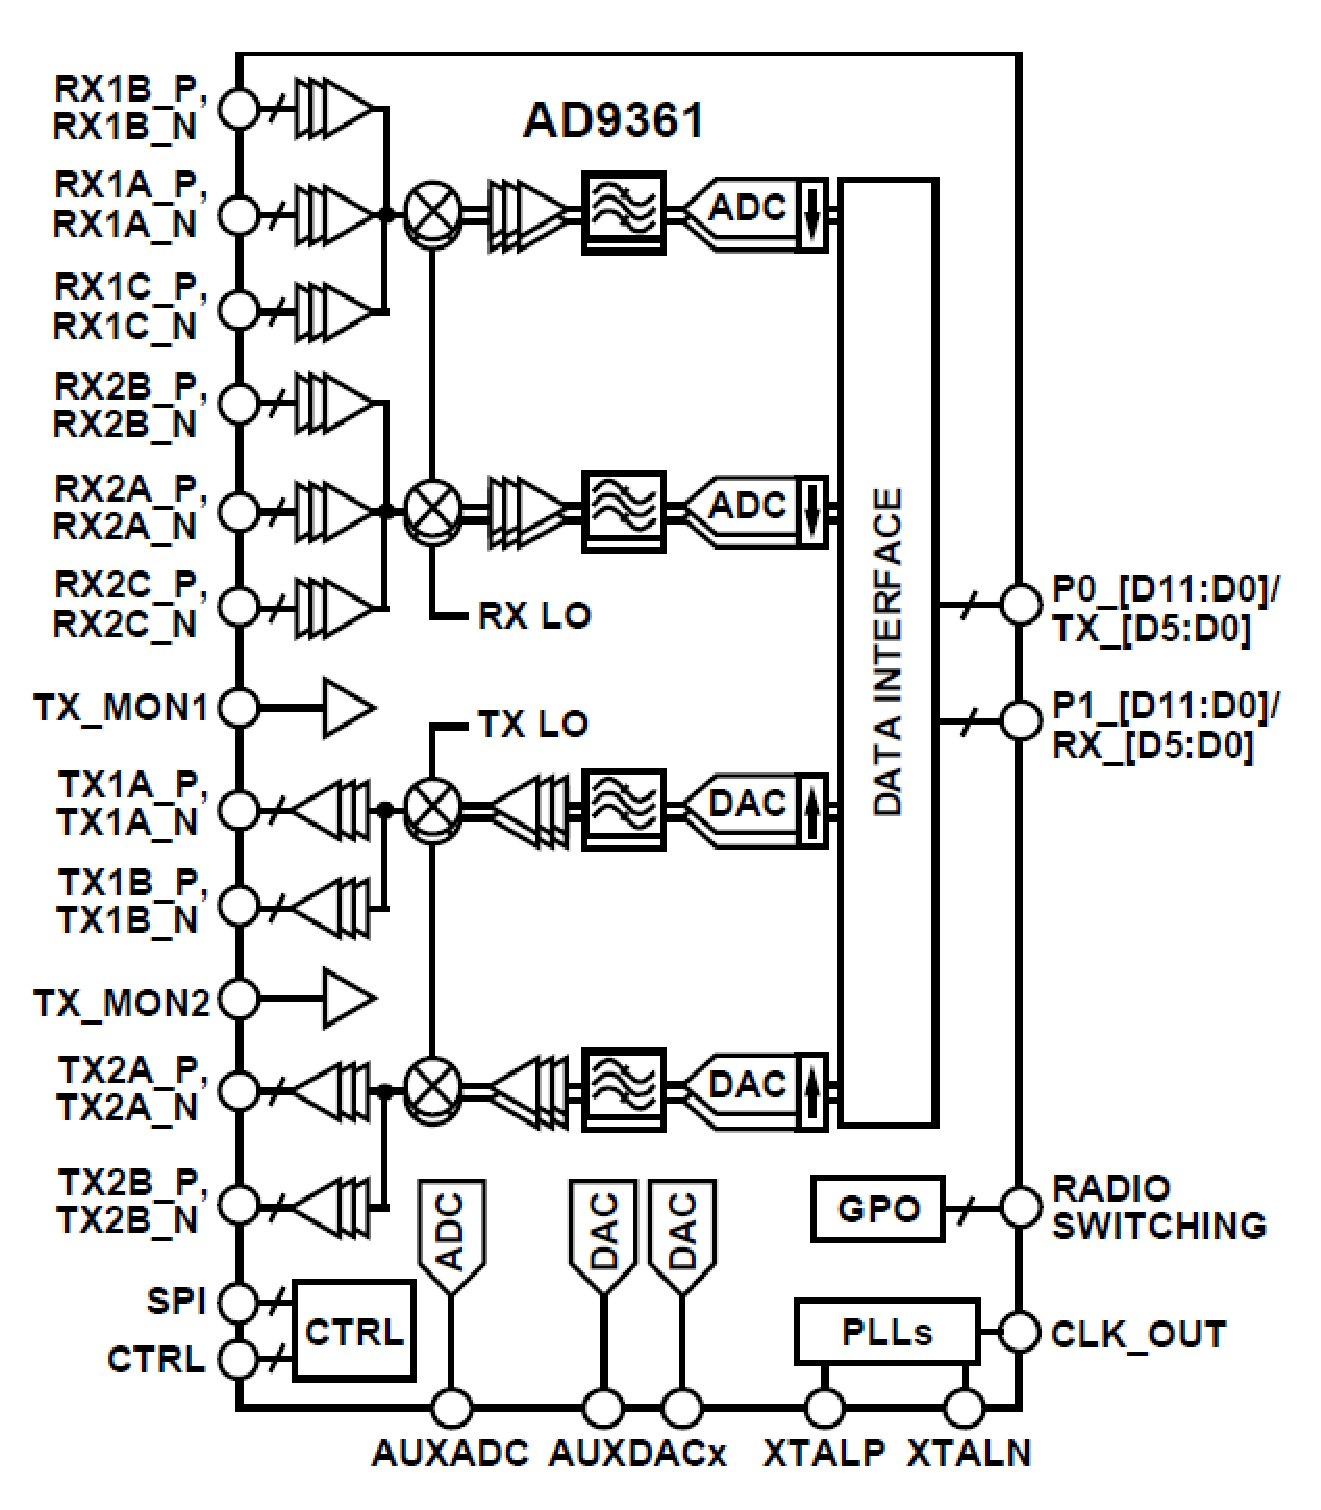
\includegraphics[width=0.65\textwidth]{./figures/ad9361_functional_diagram}
    \caption{ AD9361 Functional Block Diagram
    \label{fig:ad9361func}}
\end{figure}

\subsection{Receiver}

The receiver section has all the blocks necessary to receive analog RF signals and convert them to digital data which can be used by the BBP. there are two independently controlled channels that share same frequency synthesizer. This characteristic makes possible to the AD9361 to operate in MIMO systems.

Each channel has 3 inputs which can be multiplexed into the signal chain, making possible to use the AD9361 into systems with multiple antenna inputs. The Receiver is a direct conversion system that contains a Low noise amplifier (LNA) , followed by a matched in-phase and quadrature amplifier, mixers, and band shaping filters that down convert received signals to baseband for digitization. External LNAs can also be interfaced to the AD9361 allowing more flexibility in the design.
The receiver signal path passes downconverted signals (I and Q), which are schematically identical to each other,  to the baseband (BB) receiver section. The BB section is composed by two programmable low-pass filters, with programmable corner frequency for each filter, 12-bit ADC and four stages of decimating filters, each of the four decimation filters can be bypassed. 
The gain control is achieved by a preprogrammed gain index map, a lookup table for example, this map distributes gain in order to achieve optimal performance at each level. This optimal behavior can be achieved by enabling AGC, which can run in two modes, fast and slow gain control. This allow for the BBP to make gain adjustments as needed.
Each channel also contains independent RSSI measurement capability, DC offset tracking and all other circuitry needed for self-calibration.

The receiver ADC is a 12-bit sigma-delta ($\Sigma-\Delta$) ADC which allows adjustable sample rates. This ADC produces data streams from the received signals and such digitalized signals can be conditioned further by a series of decimation filters and a 128-tap FIR filter with additional decimation settings.
The sampling rate of each digital filter is adjustable through changes in the decimation factors to produce the needed data rate.

In short, the Receiver chain has:

\begin{itemize}
	\item LNA - Low noise Amplifier
	\item Matched in-phase amplifier;
	\item Quadrature Amplifier;
	\item Band Shaping Filters;
	\item Analog low pass filters;
	\item 12-bit DAC;
	\item 4 stages of decimation filters (128-tap FIR filters);
	\item Automatic gain Control;
\end{itemize}

\begin{figure}[htbp]
    \centering
    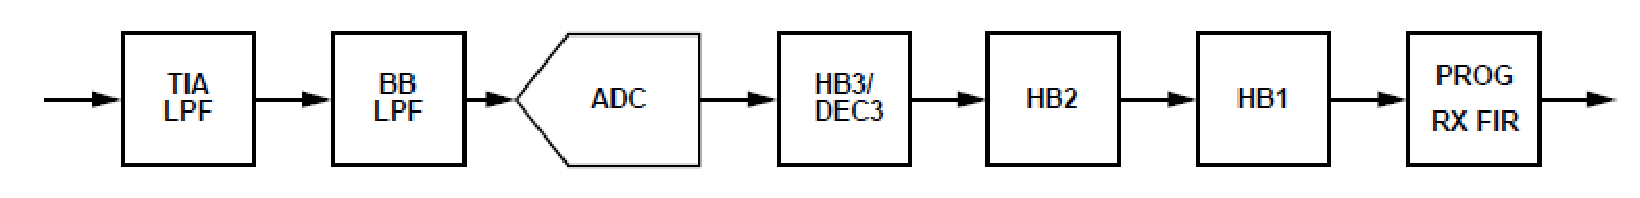
\includegraphics[width=0.65\textwidth]{./figures/rx_chain}
    \caption{ Receiver Signal Path
    \label{fig:rxchain}}
\end{figure}


\subsection{Transmitter}

Like the receiver section, the transmitter section contains two identical and independently controller channels, which share the same frequency synthesizer,  that provide all digital signal processing, mixed signal and RF blocks necessary to implement a direct conversion system from digital data to RF.
The Tx signal path receives from the BBP 12-bit 2s complement I-Q format data in the digital interface and each channel goes through a 128-tap FIR filter with interpolation options, which is fully programmable. Then the signal goes through a series of additional interpolation filters that manipulates the signal with additional filtering and data rate interpolation before reaching the 12-bit DAC, note that all these filtering and interpolation steps can be bypassed if desired.
Each 12-bit DAC has an adjustable sampling rate and its analog output passes through to low pass filters to remove any sampling artifacts before going to the RF mixer, these low pass filters corner frequencies can be programmable too. After all these filtering and analog conversion steps, the I and Q signals are recombined and modulated in the carrier frequency, which can be adjusted by changing the synthesizer frequency. These analog combined signals passes through additional analog filters for better band shaping and then it can be transmitted to the output amplifier. Each Transmitting channel provides wide attenuation adjustment range with fine granularity in order to optimize SNR.

\begin{figure}[htbp]
    \centering
    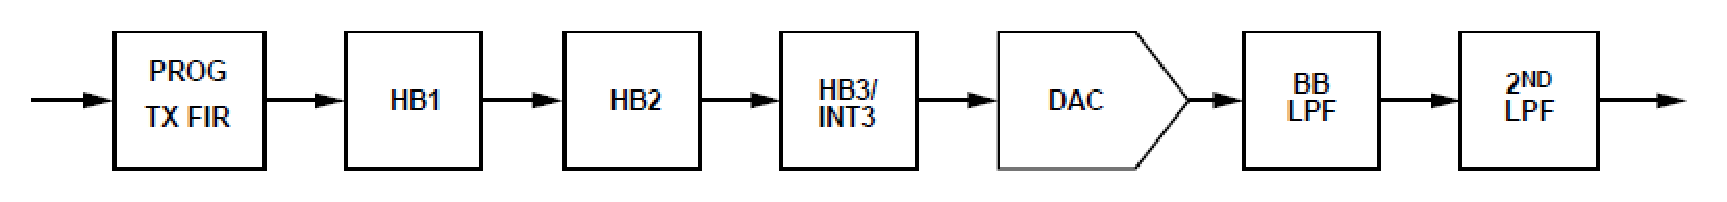
\includegraphics[width=0.65\textwidth]{./figures/tx_chain}
    \caption{ Transmitter Signal Path
    \label{fig:txchain}}
\end{figure}


Identical to the receiver chain, the transmitter chain has also built-in self-calibration circuitry into each transmitting channel providing an automatic real-time adjustment. The transmitter also provides a TX monitor block for each channel, this block monitors the transmission output and routes it back through an unused receiver channel to the BBP for signal monitoring, but these monitoring option is only available in TDD mode operation while the receiver is idle.

In short the transmission chain has:

\begin{itemize}
	\item 128-tap FIR filters;
	\item Interpolation Filters;
	\item 12-bit DAC;
	\item Analog Low-pass Filters;
	\item Additional band shaping analog filters;
	\item Attenuation adjustment;
	\item self-calibration circuits;
	\item Tx signal Monitor.
\end{itemize}

\begin{figure}[htbp]
    \centering
    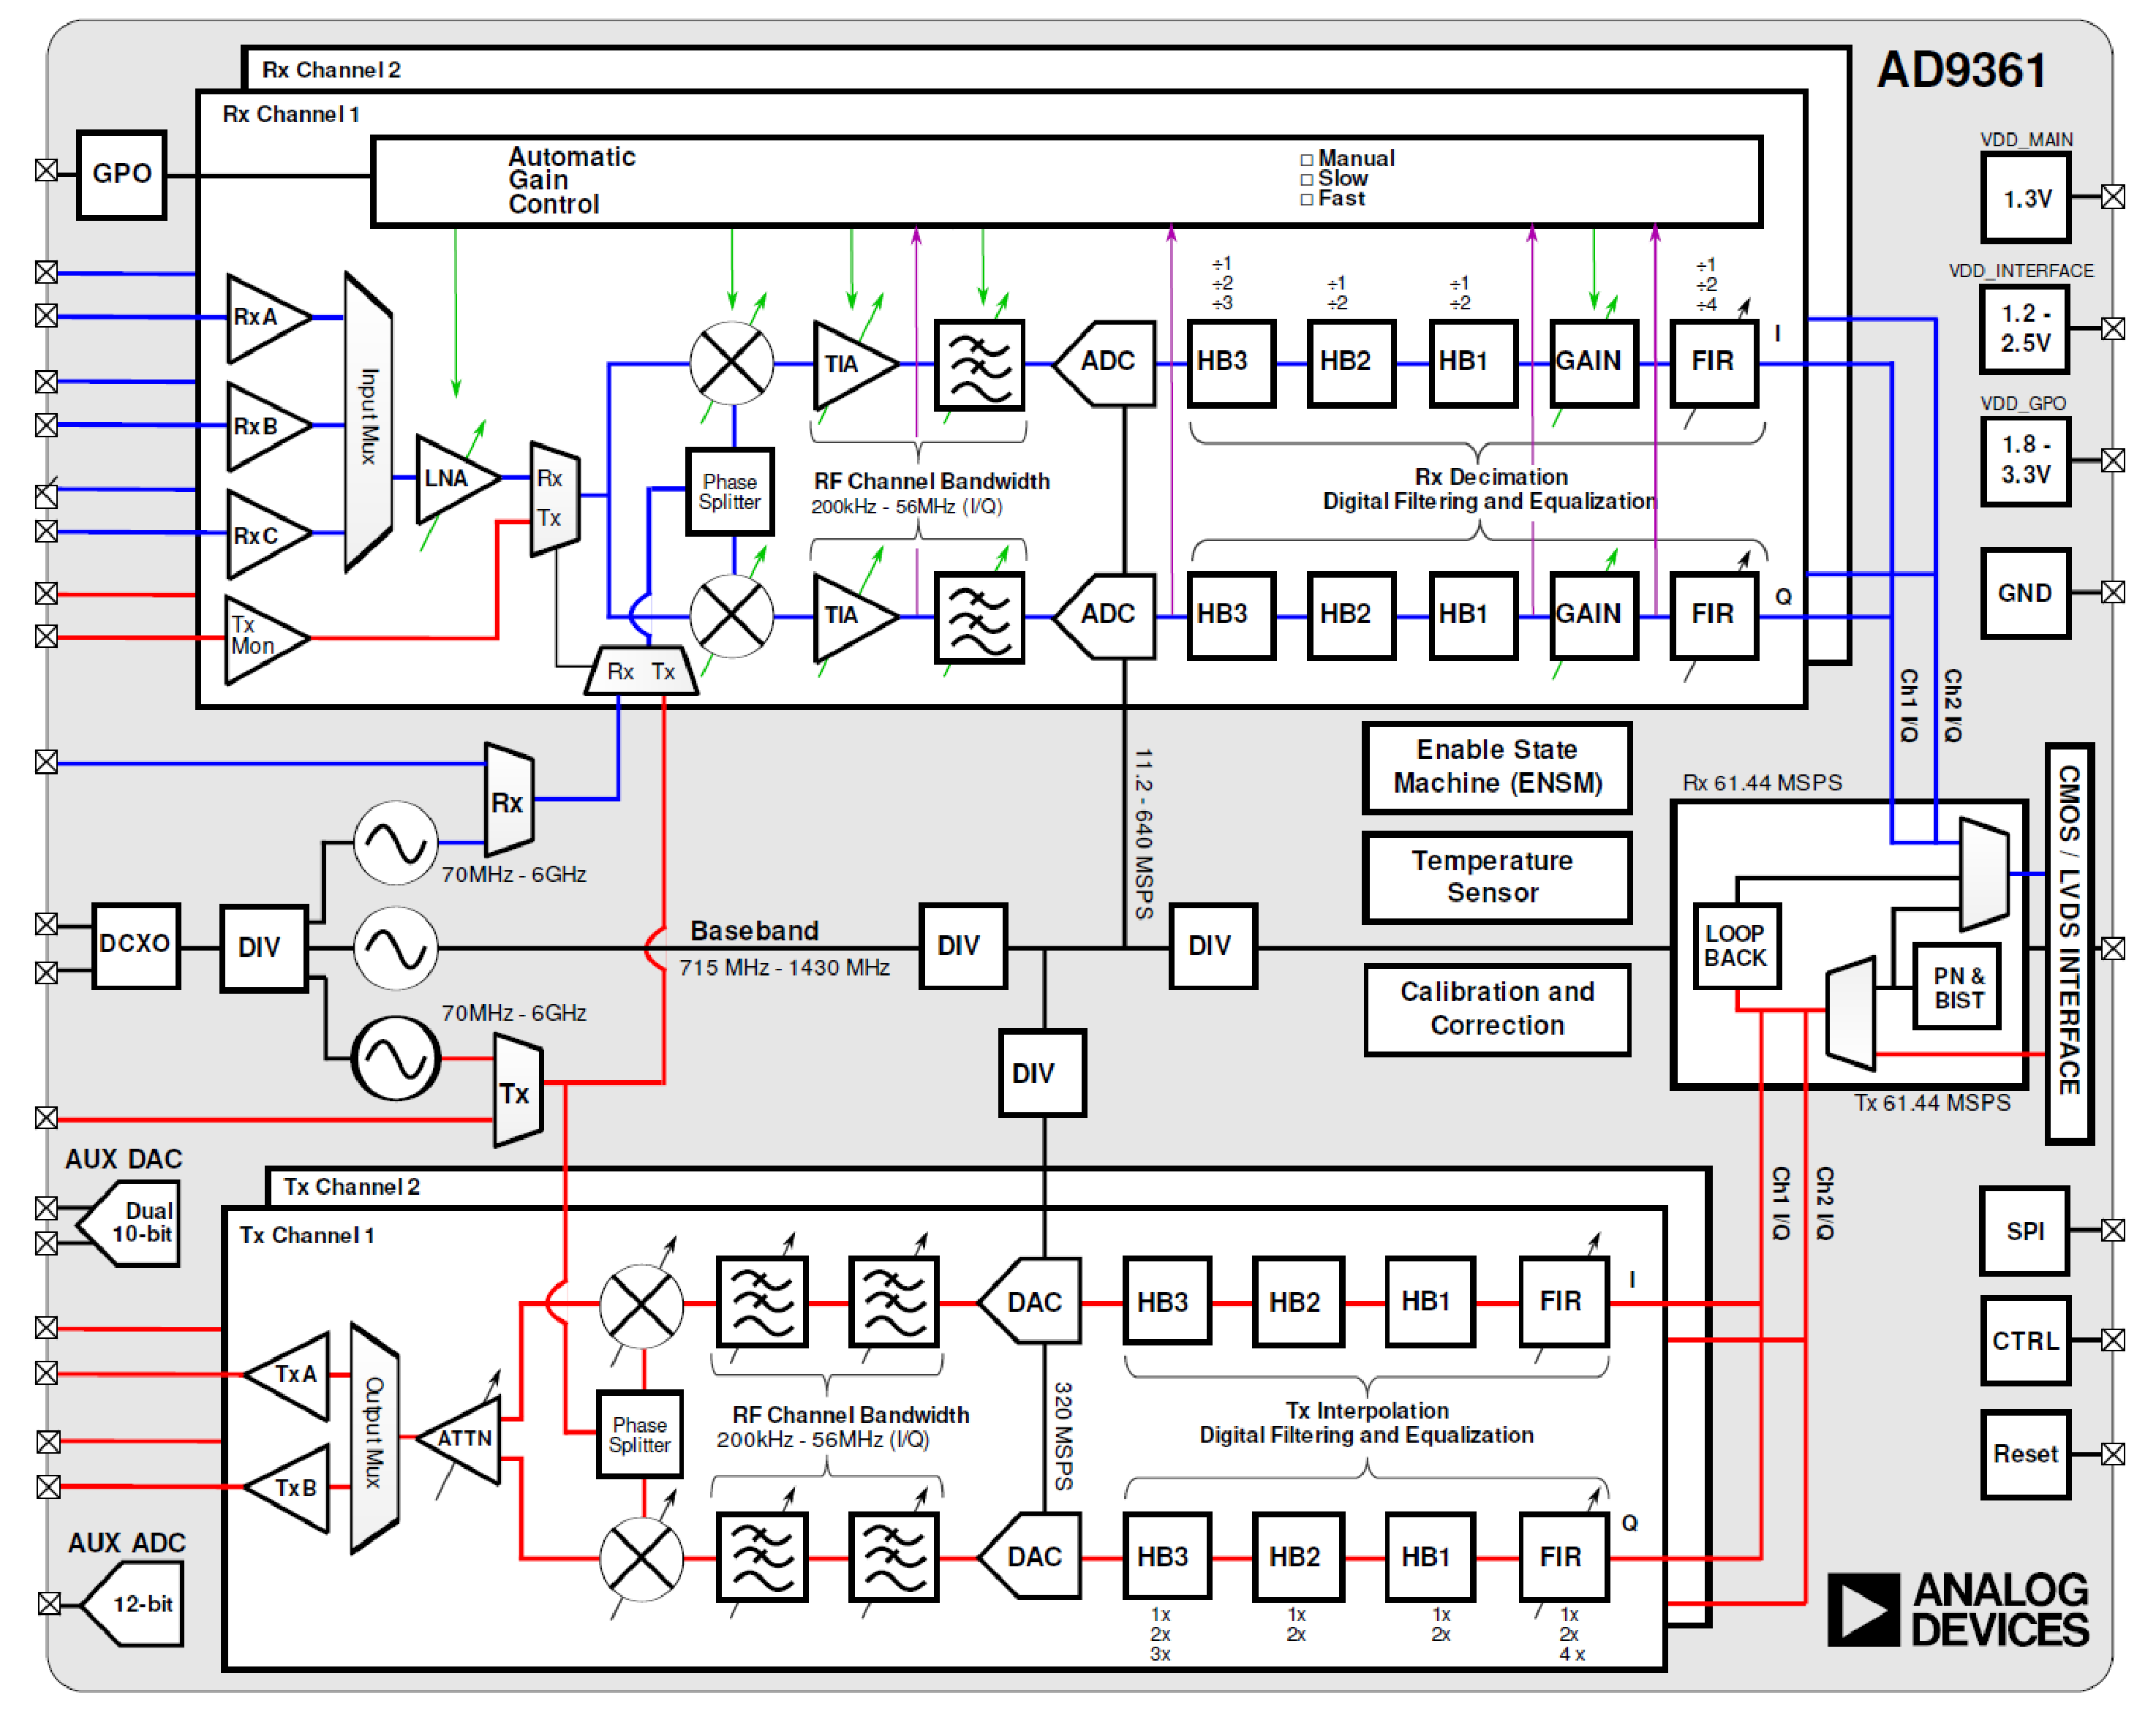
\includegraphics[width=0.65\textwidth]{./figures/ad9361_block_diagram}
    \caption{ AD9361 Block Diagram
    \label{fig:ad9361blk}}
\end{figure}

\subsection{Filtering}

In both receiver and transmitter there are:
\begin{description}
	\item[Receiver] \hfill \\
	\begin{itemize}
		\item Low pass filter : band shape to reduce adjacent-channel interference.
		\item Decimation Filter: up convert from the digital baseband rate (64.11MSPS max) to the actual ADC (640MSPS) rate.
	\end{itemize}
	\item[Transmitter] \hfill \\
\begin{itemize}
		\item Low pass filter : remove sampling artifacts
		\item Interpolation Filter : down convert from the digital baseband rate (64.11MSPS max) to the actual DAC (320MSPS) rate.
	\end{itemize}
\end{description}

In both digital and analog implementations these filters have impact the magnitude and the phase in passband, such behavior must be compensated in the system, and this compensation is usually done inside the 128-tap FIR filter. The FIR filter is not only used for low pass filter realization but also to compensate for magnitude and phase impacts created by the analog and digital half band filters in the desired baseband area. 

These filters depend in various other systems to work properly, such systems are sample rates, clock, data rates which sets the half band filters, and the desired RF bandwidth, which sets the analog filters. the process of loading a filter and after changing anything in the system will negatively affect the overall baseband performance. 

There is a filter too created by analog devices,which designs a low-pass filter and sets the FIR coefficients in order to ensure compensation for magnitude and phase changes in the analog or half band filters.

\subsection{Clocking}

%reescrever
The AD9361 has a series of internal PLL to generate and manipulate clock signals. There are fractional-n PLLs that generate the transmitter and receiver LO frequencies and there are the baseband PLL (BBPLL) used for the data converters, digital filters and I/O ports. All the frequency signals are generated using these PLLs clock outputs.

All the PLLs require a reference clock input and for this there is the digitally controlled oscillator (DXCO) function, which is an in-chip programmable and variable capacitor, such capacitor can tune the crystal frequency variance before entering the system, having a precision of +/- 6 ppm it results in a more accurate reference clock and can be used, if needed, for synchronization purposes. this function can also be used together with the on-chip temperature sensor to provide temperature compensation depending enviroment in which the chip will be used. For the reference clock there are two options:

\begin{description}
	\item[External Oscillator] \hfill \\
	In this option and external clock signal can be connected in the XTALP pin (Leaving the XTALP pin unconnected), this external clock frequency may vary from 10 MHz to 80 MHz. Such type of setup is needed when a wireless basestation (BTS) reference clock is locked to a master clock, and in such systems there is no or less need for clock synchronization.

	\item[Dedicated Crystal] \hfill \\
	In this option a dedicated crystal, with frequency varying from 19 MHz to 50 MHz, is connected in the XTALP and XTALN pins. This setup is usually used in wireless user equipment (UE), which do not need to be locked to a master clock but they do need to adjust periodically the LO frequency in order to maintain a connection with a BTS. The BTS periodically informs the UE of its frequency error relative to the BTS and the BBP can make adjustments to the reference clock and thus adjust the LO frequency if needed.

\end{description} 

\begin{figure}[htbp]
    \centering
    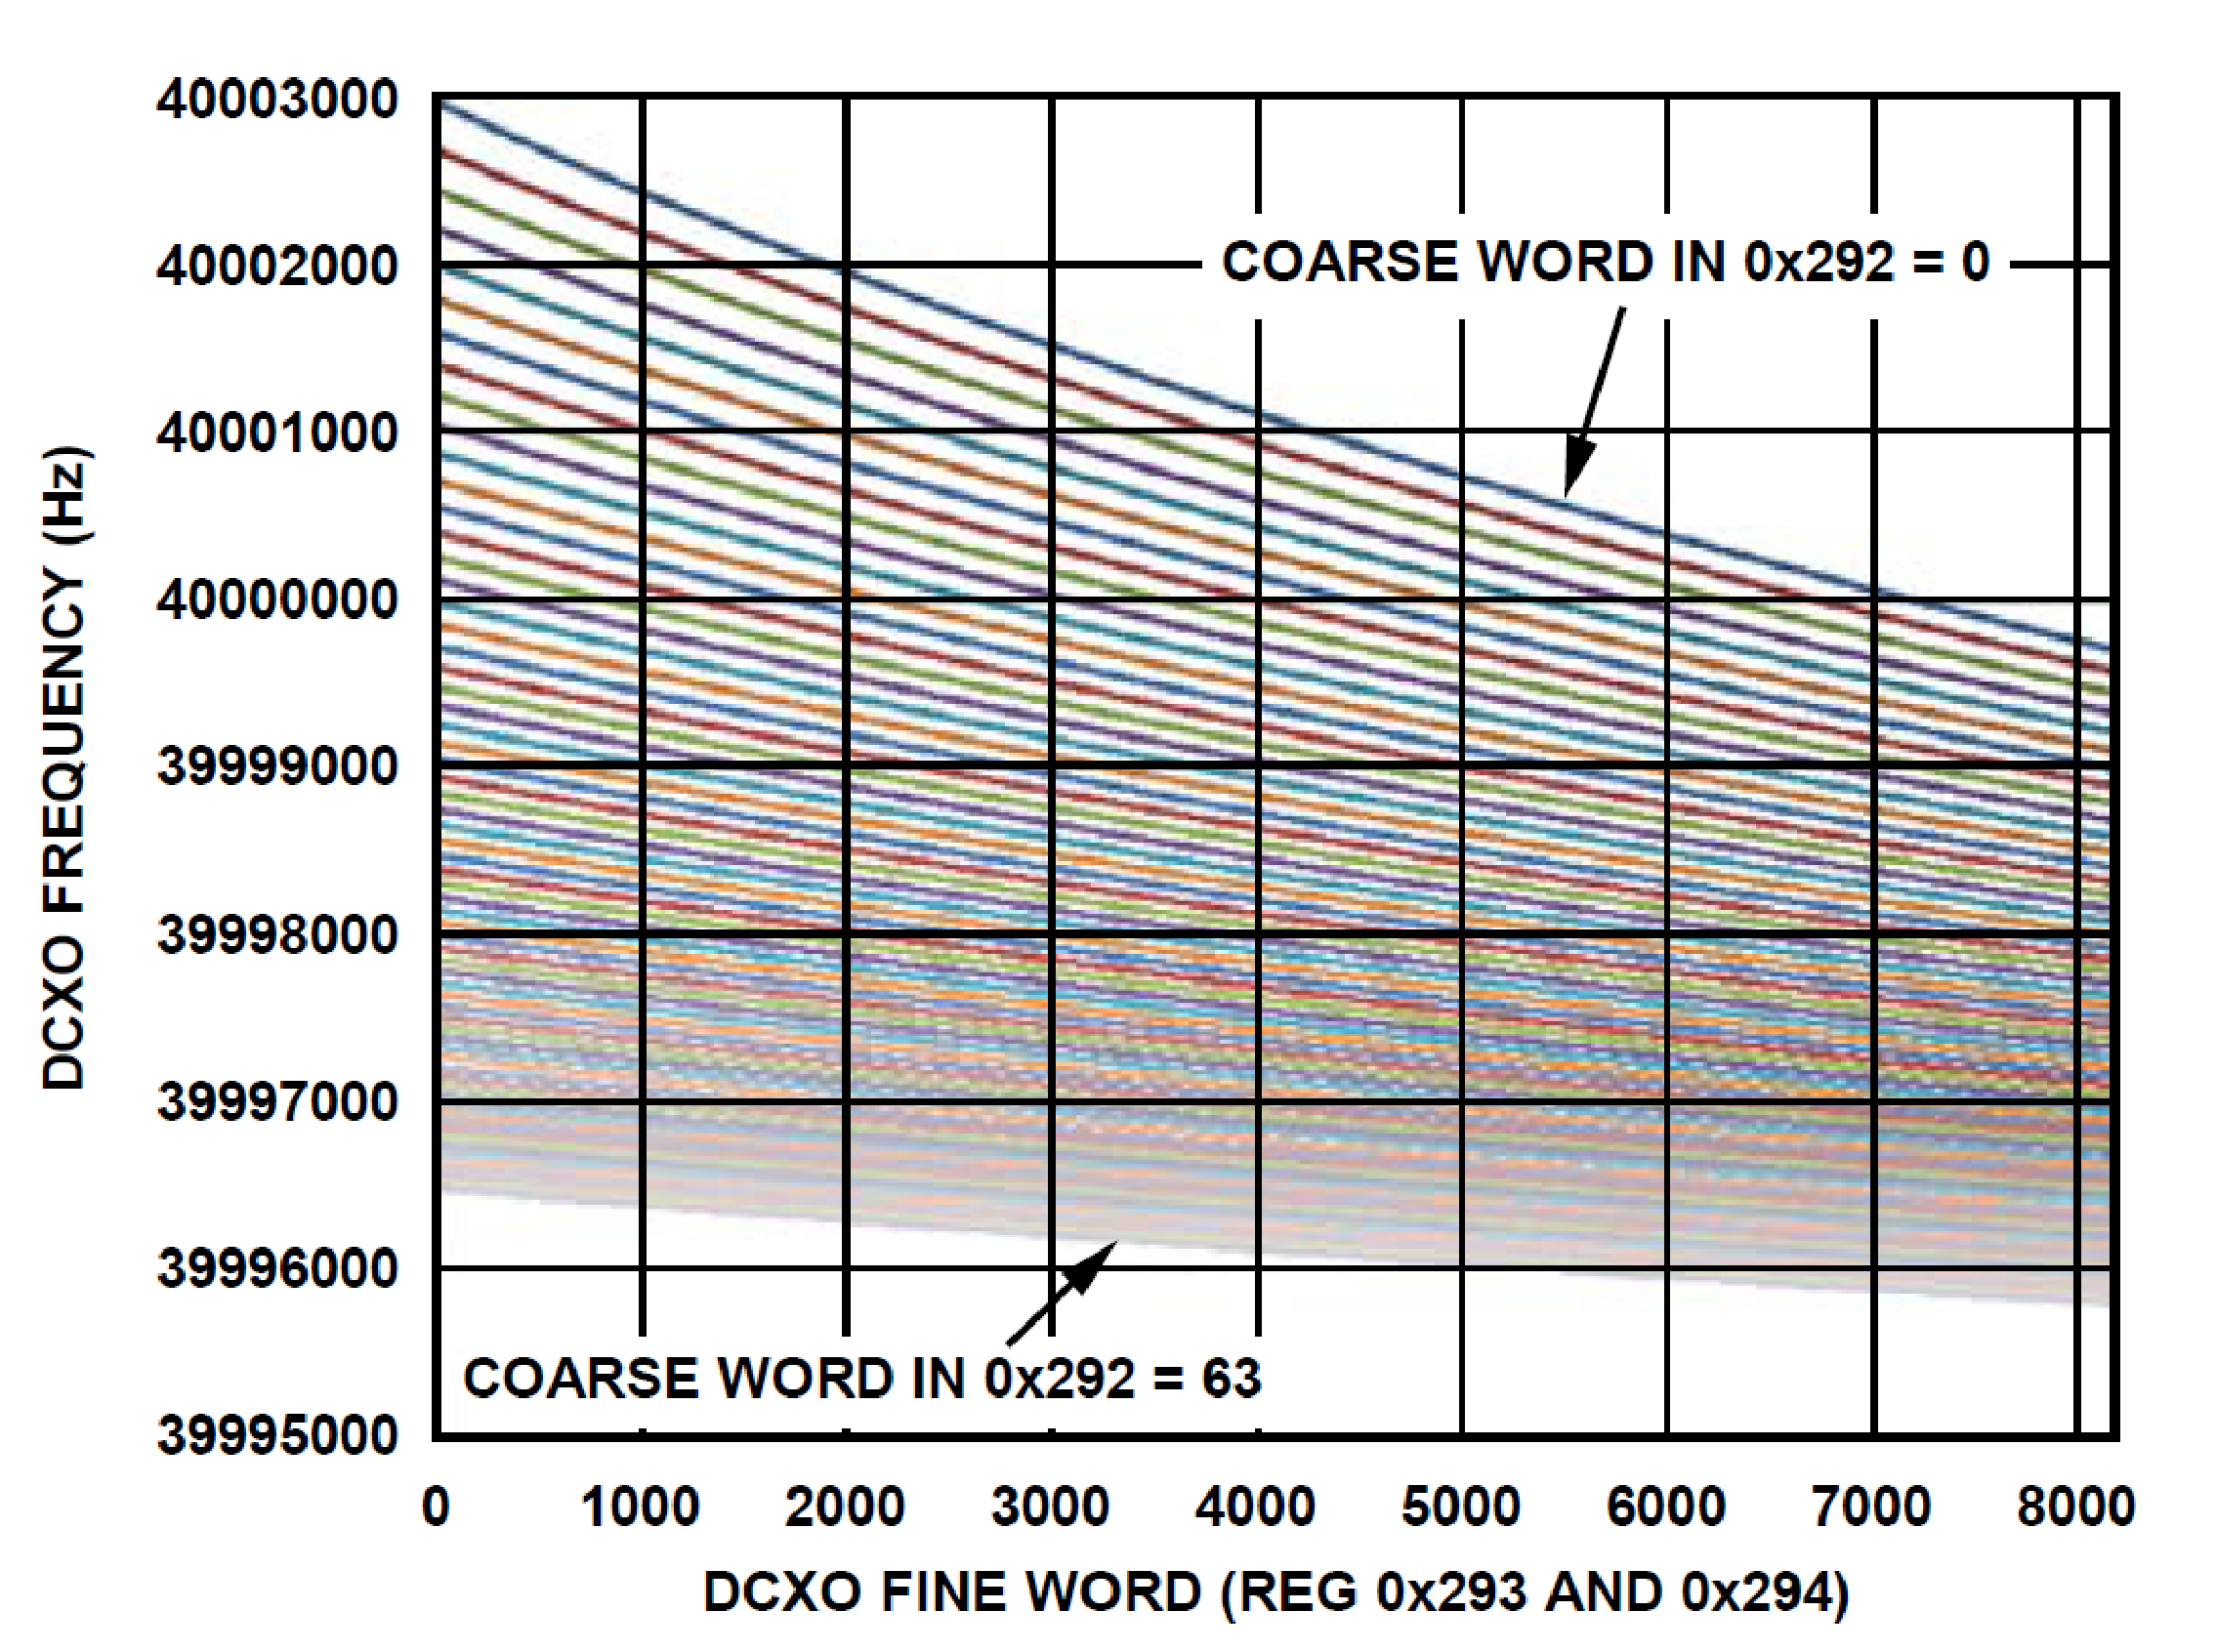
\includegraphics[width=0.65\textwidth]{./figures/dcxo_graph}
    \caption{ DCXO Behavior Graph
    \label{fig:pll}}
\end{figure}

\subsection{Synthesizers}

\begin{description}
	\item[RF PLLs] \hfill \\
	The AD9361 contains two identical synthesizers to generate the required LO signals for the RF signal path, one for the receiver and one for the transmitter. The PLL synthesizers are fractional-n PLLs with completely integrated VCOs and loop filters, requiring no other external components. In TDD operation mode, the synthesizers turn ON and OFF appropriate for the TX and RX frames, however in FDD TX PLL and RX PLL are activated at the same time.

	\item[BB PLL] \hfill \\
	The AD9361 contains also a baseband PLL synthesizer, which generate all the baseband related clock signals. The BBPLL feeds all the baseband related clock signals to ADC, DAC (Sampling Clock), DATA\_CLK signal and all data framing signals. This PLL has a frequency range from 700 Mhz to 1400 Mhz, and can be changed based on system requirements.

\end{description}

\begin{figure}[htbp]
    \centering
    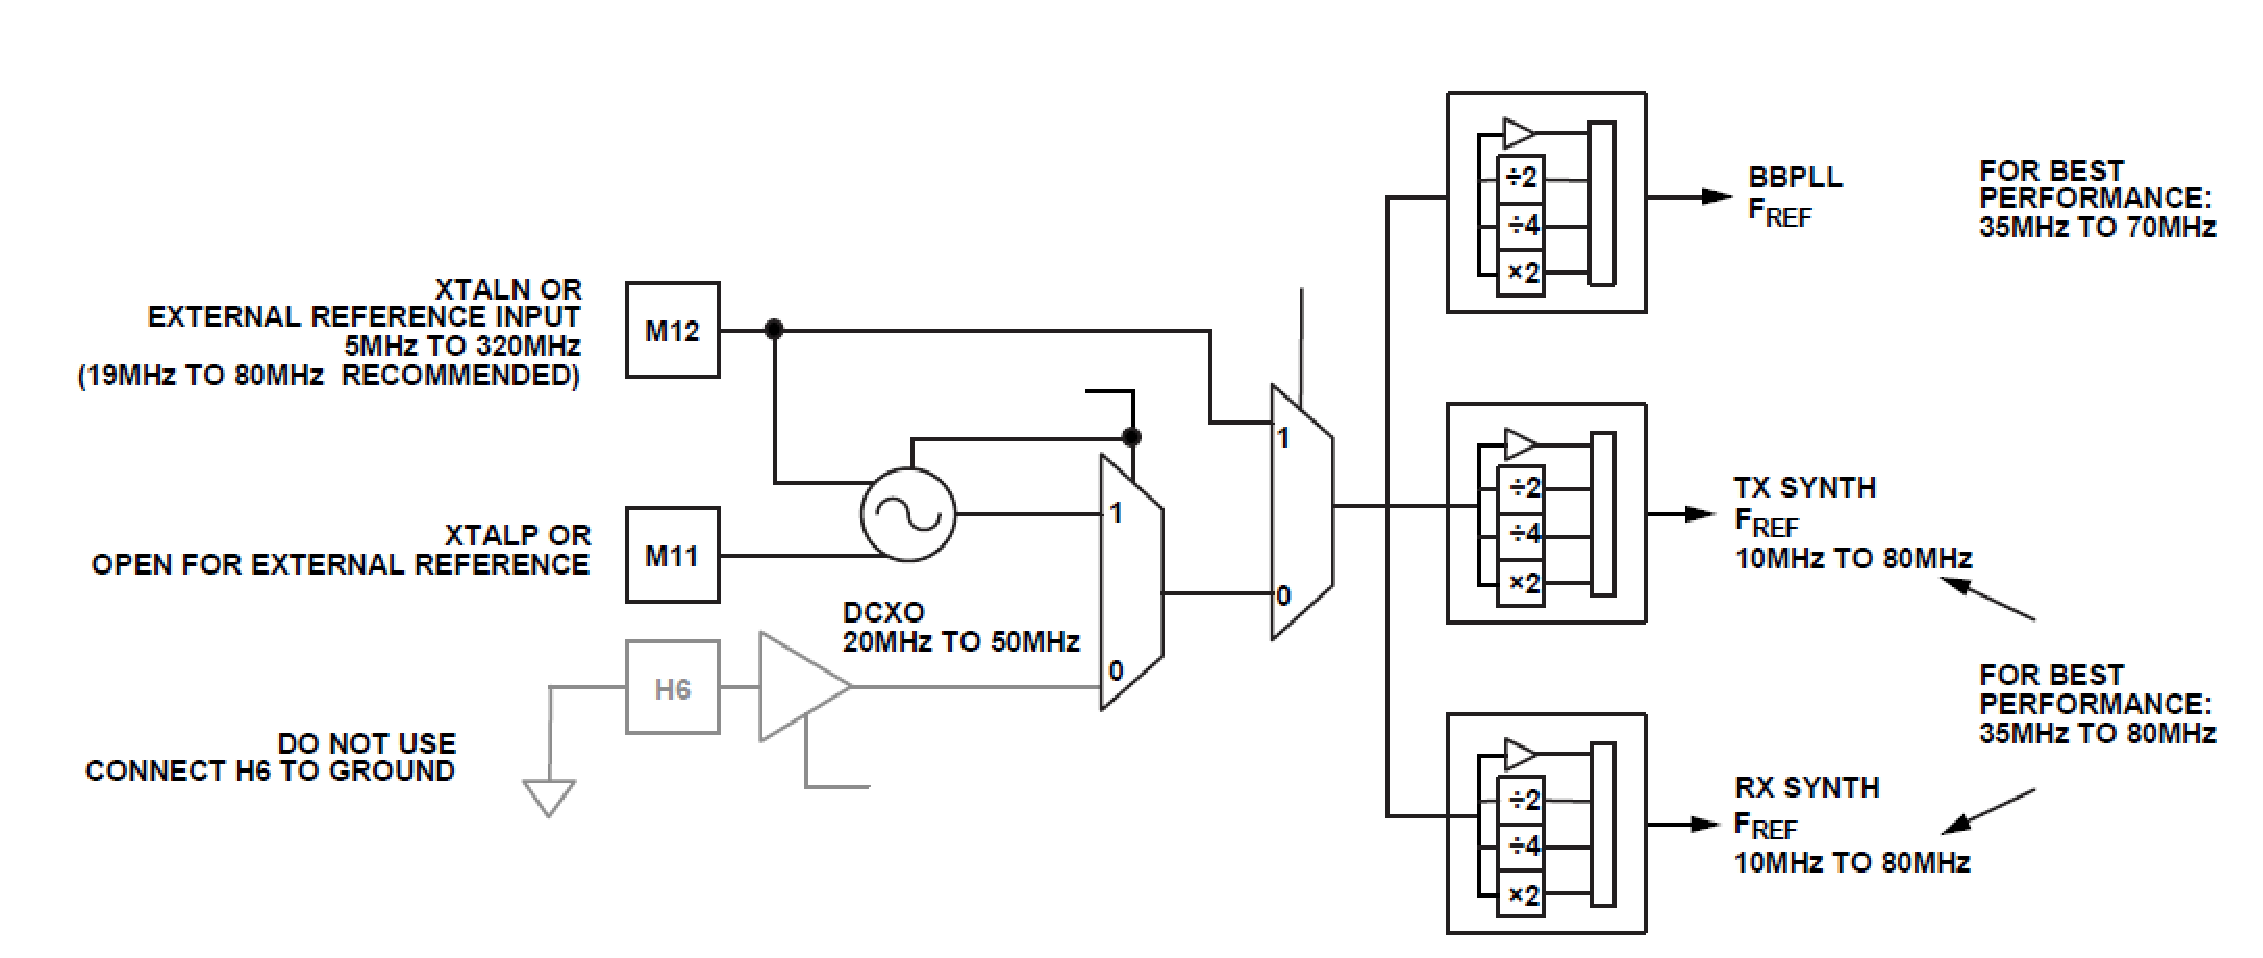
\includegraphics[width=0.65\textwidth]{./figures/pll_ref_block}
    \caption{ AD9361 PLL Reference Block Diagram
    \label{fig:pll}}
\end{figure}

\subsection{Digital Data Interface}

The AD9361 uses parallel data ports to transfer data between the device and the BBP. These data ports can be configured either single-ended CMOS format or LVDS format (used in this work). Both formats can be configured in multiple arrangements to adequate the system requirements for data transfer and connections. These arrangements can be of single port data bus, dual port data bus, single data rate, double data rate and other various combinations compatible with the device.\\
Bus transfers are controlled using hardware handshake signalling, these two ports can be operated in TDD (bidirectional) or FDD (full duplex) where half of the bits are used for transmitting and the other half is used for receiving. The interface can also be configured to use only one of the data ports ( usually used in applications that do not require high data rates or samples).\\
The communication between the BBP processor and the AD9361 rely on some signals to properly work, which are DATA\_CLK, FB\_CLK and RX\_FRAME, its operation is detailed below:

\begin{description}
	\item[DATA\_CLK Signal] \hfill \\
	RX sends the signal DATA\_CLK to the BBP, which can be used when receiving data. DATA\_CLK can be used to control data sampling time, which can be single data rate (data is captured on rising clock edge) or double data rate (data is captured on both rising and falling clock edges). This can be applied using single or dual data port.

	\item[FB\_CLK Signal] \hfill \\
	The FB\_CLK signal must have the same frequency and duty cycle as DATA\_CLK and like DATA\_CLK it is used as timing reference for the interface. FB\_CLK allows source synchronous with rising edge capture for burst control signals and can be used like DATA\_CLK for rising edge, single data rate mode or in both edge capture, double data rate mode for transmit signal bursts.

	\item[RF\_FRAME Signal] \hfill \\
	The RF\_FRAME signal is generated by the device whenever the receiver outputs valid data. RF\_FRAME has two modes:
	\begin{itemize}
		\item \textbf{Level Mode:} RF\_FRAME stays high as long as the data is valid.
		\item \textbf{Pulse Mode:} RF\_FRAME pulses with 30% duty cycle.
	\end{itemize}
	The BBP must provide a TX\_FRAME that indicates beginning of a valid data transmission with a rising edge. The TX\_FRAME operates similarly as the RF\_FRAME, on Level Mode or Pulse Mode.

\end{description}

\begin{figure}[htbp]
    \centering
    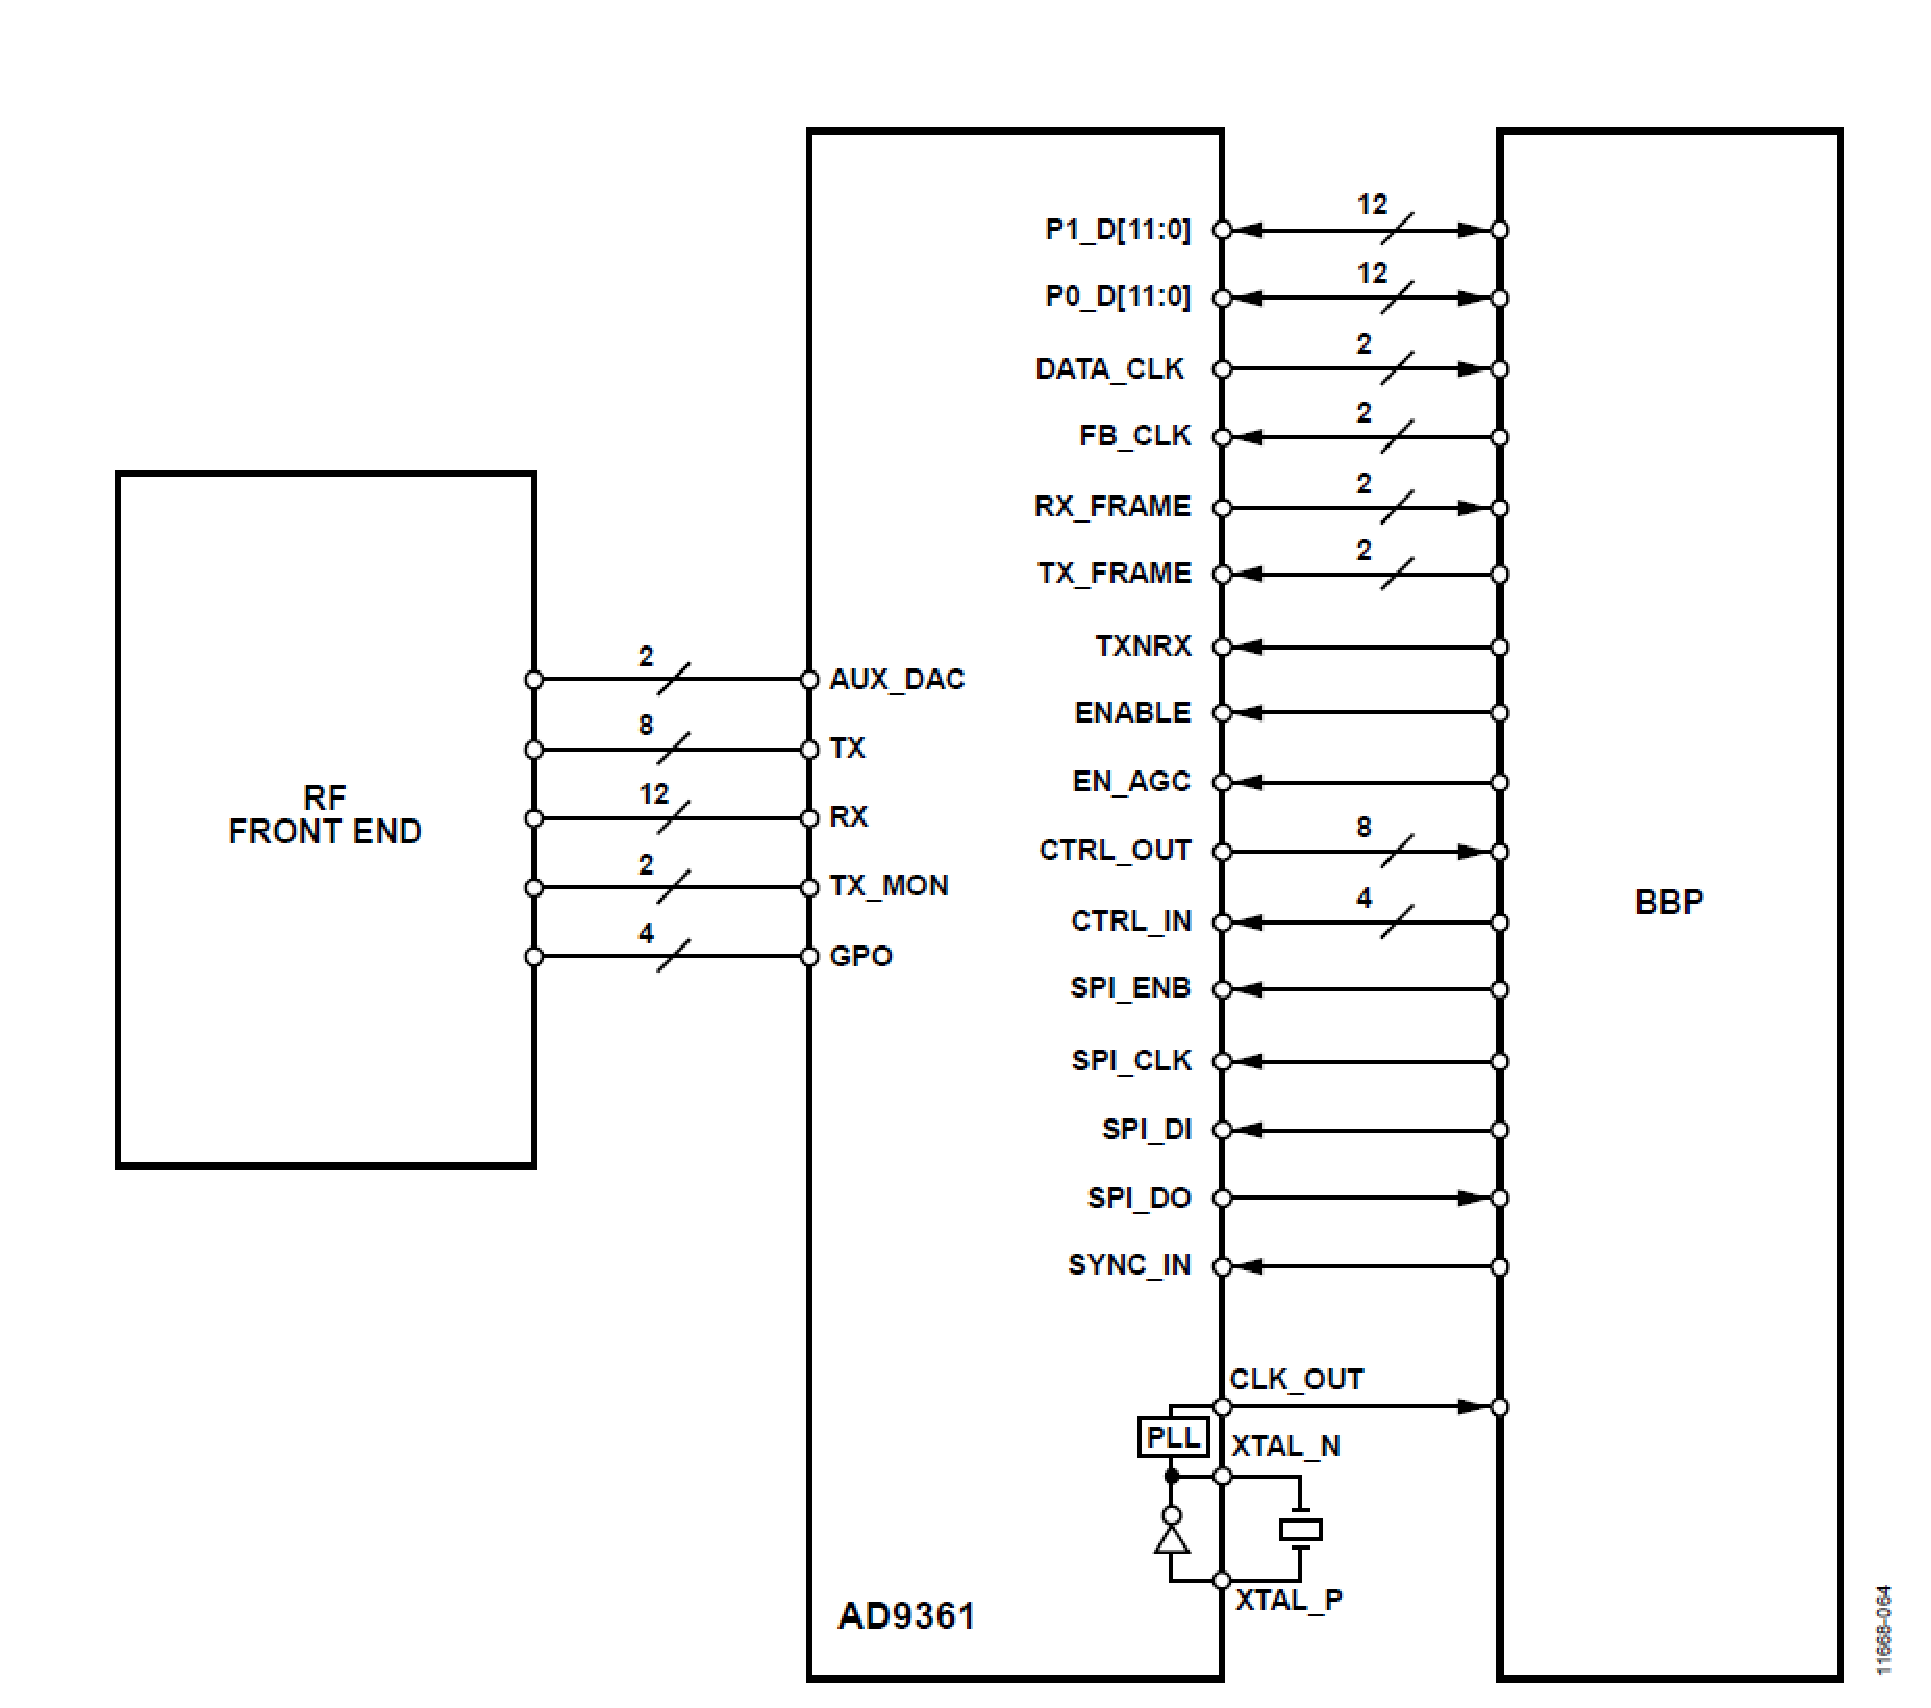
\includegraphics[width=0.65\textwidth]{./figures/ad9361_digital_interface}
    \caption{ AD9361 Digital Data Interface
    \label{fig:ad9361diginterface}}
\end{figure}


\subsection{Enable State Machine}

The AD9361 has an Enable State Machine (ENSM) which allows real-time control over the current state of the device. The device can be place in several states like:

\begin{itemize}
		\item \textbf{Wait:} Power save, synthesizers disabled.
		\item \textbf{Sleep:} Wait with all clocks and BBPLLs disabled.
		\item \textbf{TX:} TX chain enabled.
		\item \textbf{RX:} RX chain enabled.
		\item \textbf{FDD:}TX and RX chains enabled.
		\item \textbf{Alert:} Synthesizers enabled.
	\end{itemize}
	This ENSM can be controlled either by SPI or PIN (GPIO for example), where the SPI control mode is for a non real-time operation and the PIN control mode is for a much faster and real-time control.
	

\begin{description}
	\item[SPI Control Mode] \hfill \\
	In SPI control mode, the BBP writes registers asynchronously by using SPI protocol to access the addresses, and by writing these registers the state machine advances the current state to the next state. SPI communication is considerece asynchronous to the DATA\_CLK because the SPI\_CLK can be derived from another clock source, where BBP and the device does not share the same clock source. This control method is recommended when there is no need for a real-time control.

	\item[Pin Control Mode] \hfill \\
	In Pin control mode, there are pins dedicated to activate some states of the ENSM, like ENABLE pin and TXNRX pin, this mode allows a real-time control of the current state. This method is recommended in a system where the BBIC has extra pins to spare with the real-time control outputs, this 2-wire interface can control the state of the device.
	To advance the current state to the next state of the ENSM, the enable function of the ENABLE pin can be driven by either pulse or level,if the pulse is used the minimum width of the pulse needs to be equal as the FB\_CLK cycle.
	In FDD mode, the ENABLE and TXNRX pins can be remapped to be used as real-time control of the TX and RX data transfers. In this mode ENABLE enables or disables the receive signal and TXNRX enables or disables the transmit signal, using such mode  causes the ENSM to be removed from the system for data flow control and is replaced by these pins.

\end{description}

\begin{figure}[htbp]
    \centering
    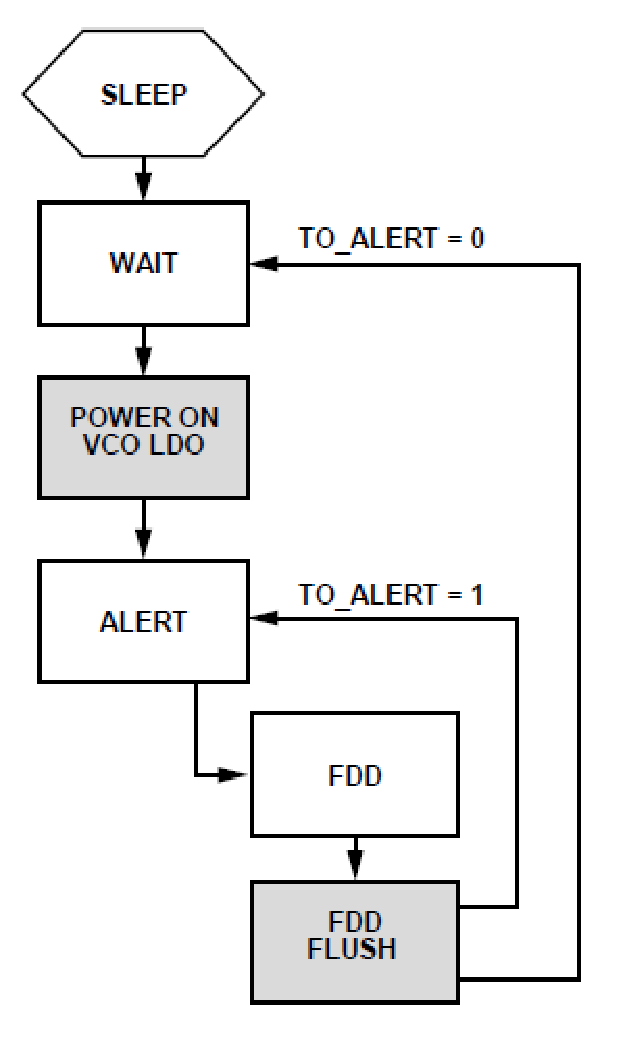
\includegraphics[width=0.65\textwidth]{./figures/fdd_ensm}
    \caption{ FDD Enable State Machine
    \label{fig:pll}}
\end{figure}

\begin{figure}[htbp]
    \centering
    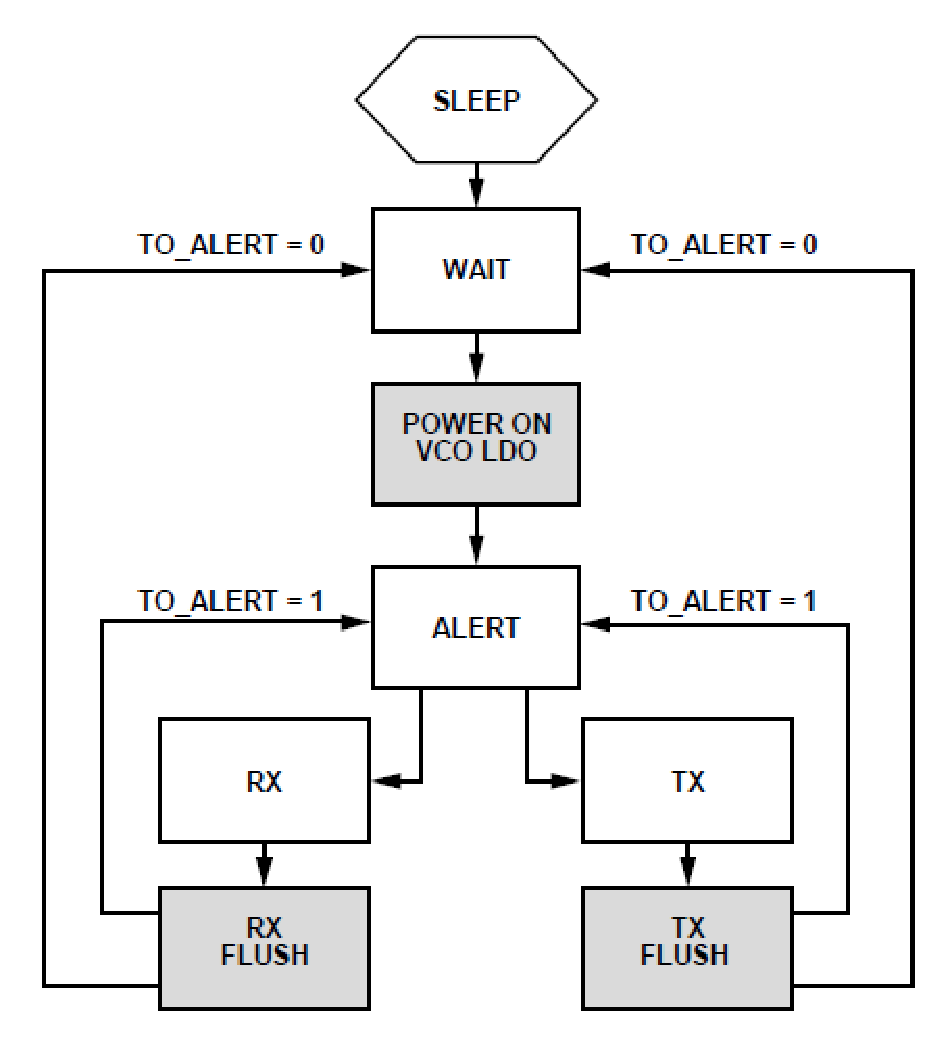
\includegraphics[width=0.65\textwidth]{./figures/tdd_ensm}
    \caption{ TDD Enable State Machine
    \label{fig:pll}}
\end{figure}


\subsection{SPI Interface}

The AD9361 uses a SPI interface for communication with the BBP. Throught SPI is possible to access all the device registers. The PSI interface can be configured as a 4-wire interface with dedicated transmit and receive pins, duplex, or as 3-wire interface with bidirectional data port. 
Write commands have a 24-bit format where the first six bits are for setting the bus direction and number of bytes to transfer, the next 10 bits set the address where the data is to be written and the final eight bits are the data to be transferred to the specific register address (MSB to LSB), a LSB-first format is also supported.
Read commands follow a similar format, the difference is that the first 16 bits are transferred on the SPI\_DI pin and the final eight are read from the AD9361, either using SPI\_DO (4-wire interface) or SPI\_DI (3-wire interface).

\subsection{Auxiliary Converters}

\begin{description}

	\item[AUXADC] \hfill \\
	The AD(361 contains an auxiliary ADC that can be used to monitor some system functions such as temperature or power output, it is a 12-bit converter and has an input range of 0V to 1.25V. The SPI can read the last value latched at the output of the ADC when it is enabled for use, there is also a multiplexer that permits to select between AUXADC and built-in temperature sensor.

	\item[AUXDAC1 and AUXDAC2] \hfill \\
	The AD(361 also has two identical auxiliary DACs which can be used to provide power amplifier (PA) bias or other system functionality. Both the DACs are 10-bit wide and have an output range of 0.5 V to 0.3V and have a current drive of 10mA. The DACs can be directly controlled by the ENSM.

\end{description}

\subsection{Applications}


\section{FMCommS2}

FMCommS2 is basically evaluation board for the AD9361 that has a FPGA Mezzanine Card (FMC) connector for interfacing with the BBP (Usually FPGA). The FMComms2 has 5 SMA connectors, 2 for Rx, 2 for Tx and one for external reference clock input. The FMComms2 provides a 2x2 RF configuration, extended from the AD9361, and has  a narrow tuning range balun, which is performance optimized for 2.4GHz.
The FMComms2 is a transceiver intended for use in RF applications such 3G or 4G BTS or SDR. Its programmability and wideband capability make it ideal for broad range of transceiver applications and make it very attractive for the new C-RAN paradigm.

\begin{figure}[htbp]
    \centering
    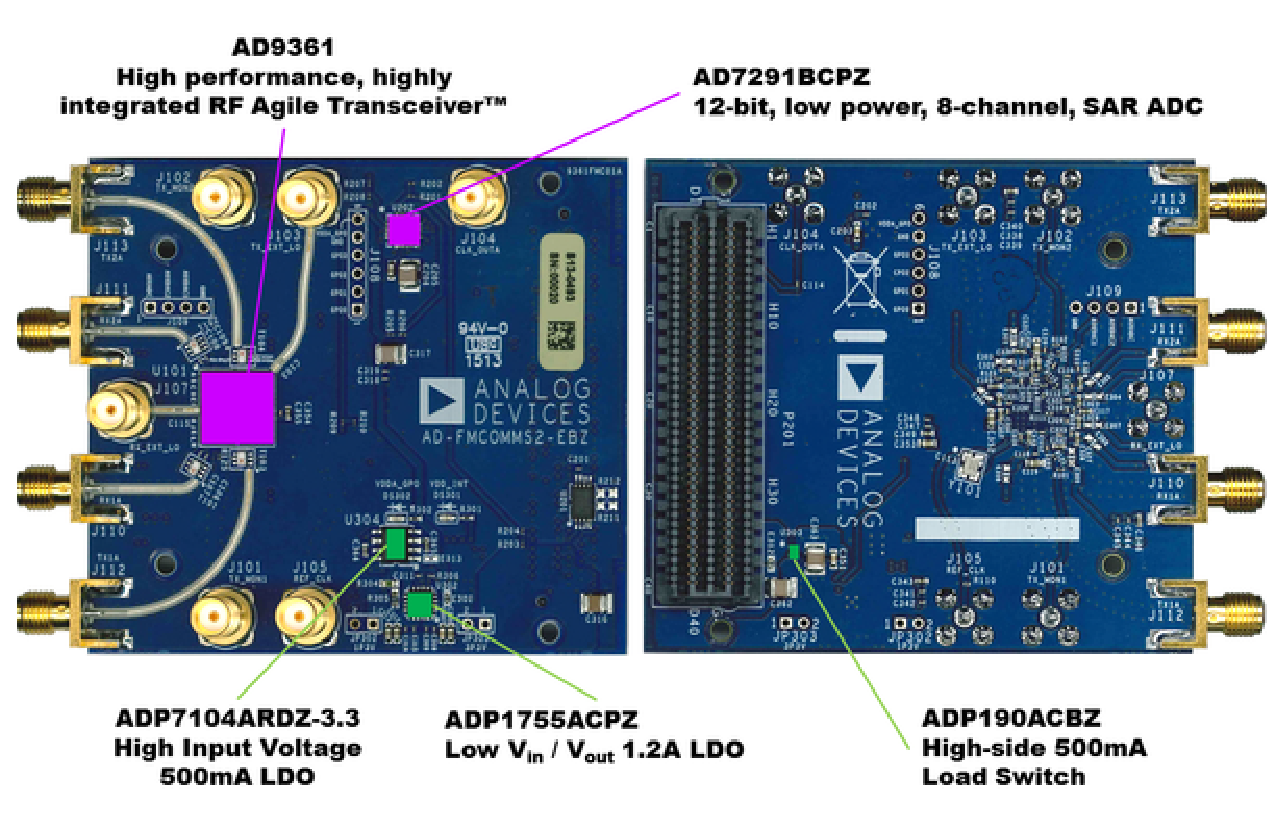
\includegraphics[width=0.65\textwidth]{./figures/fmcomms2_pic}
    \caption{ FMComms2 and its components
    \label{fig:fmcomm}}
\end{figure}


\subsection{Functional Overview}

The Block diagram show that there are 4 main functional partitions - receiver path, transmit path, clocking and power supply. Since the FMComms2 incorporates and extends the basic functionalities of the AD9361, thus the data path is fully integrated into the AD9361.

\begin{figure}[htbp]
    \centering
    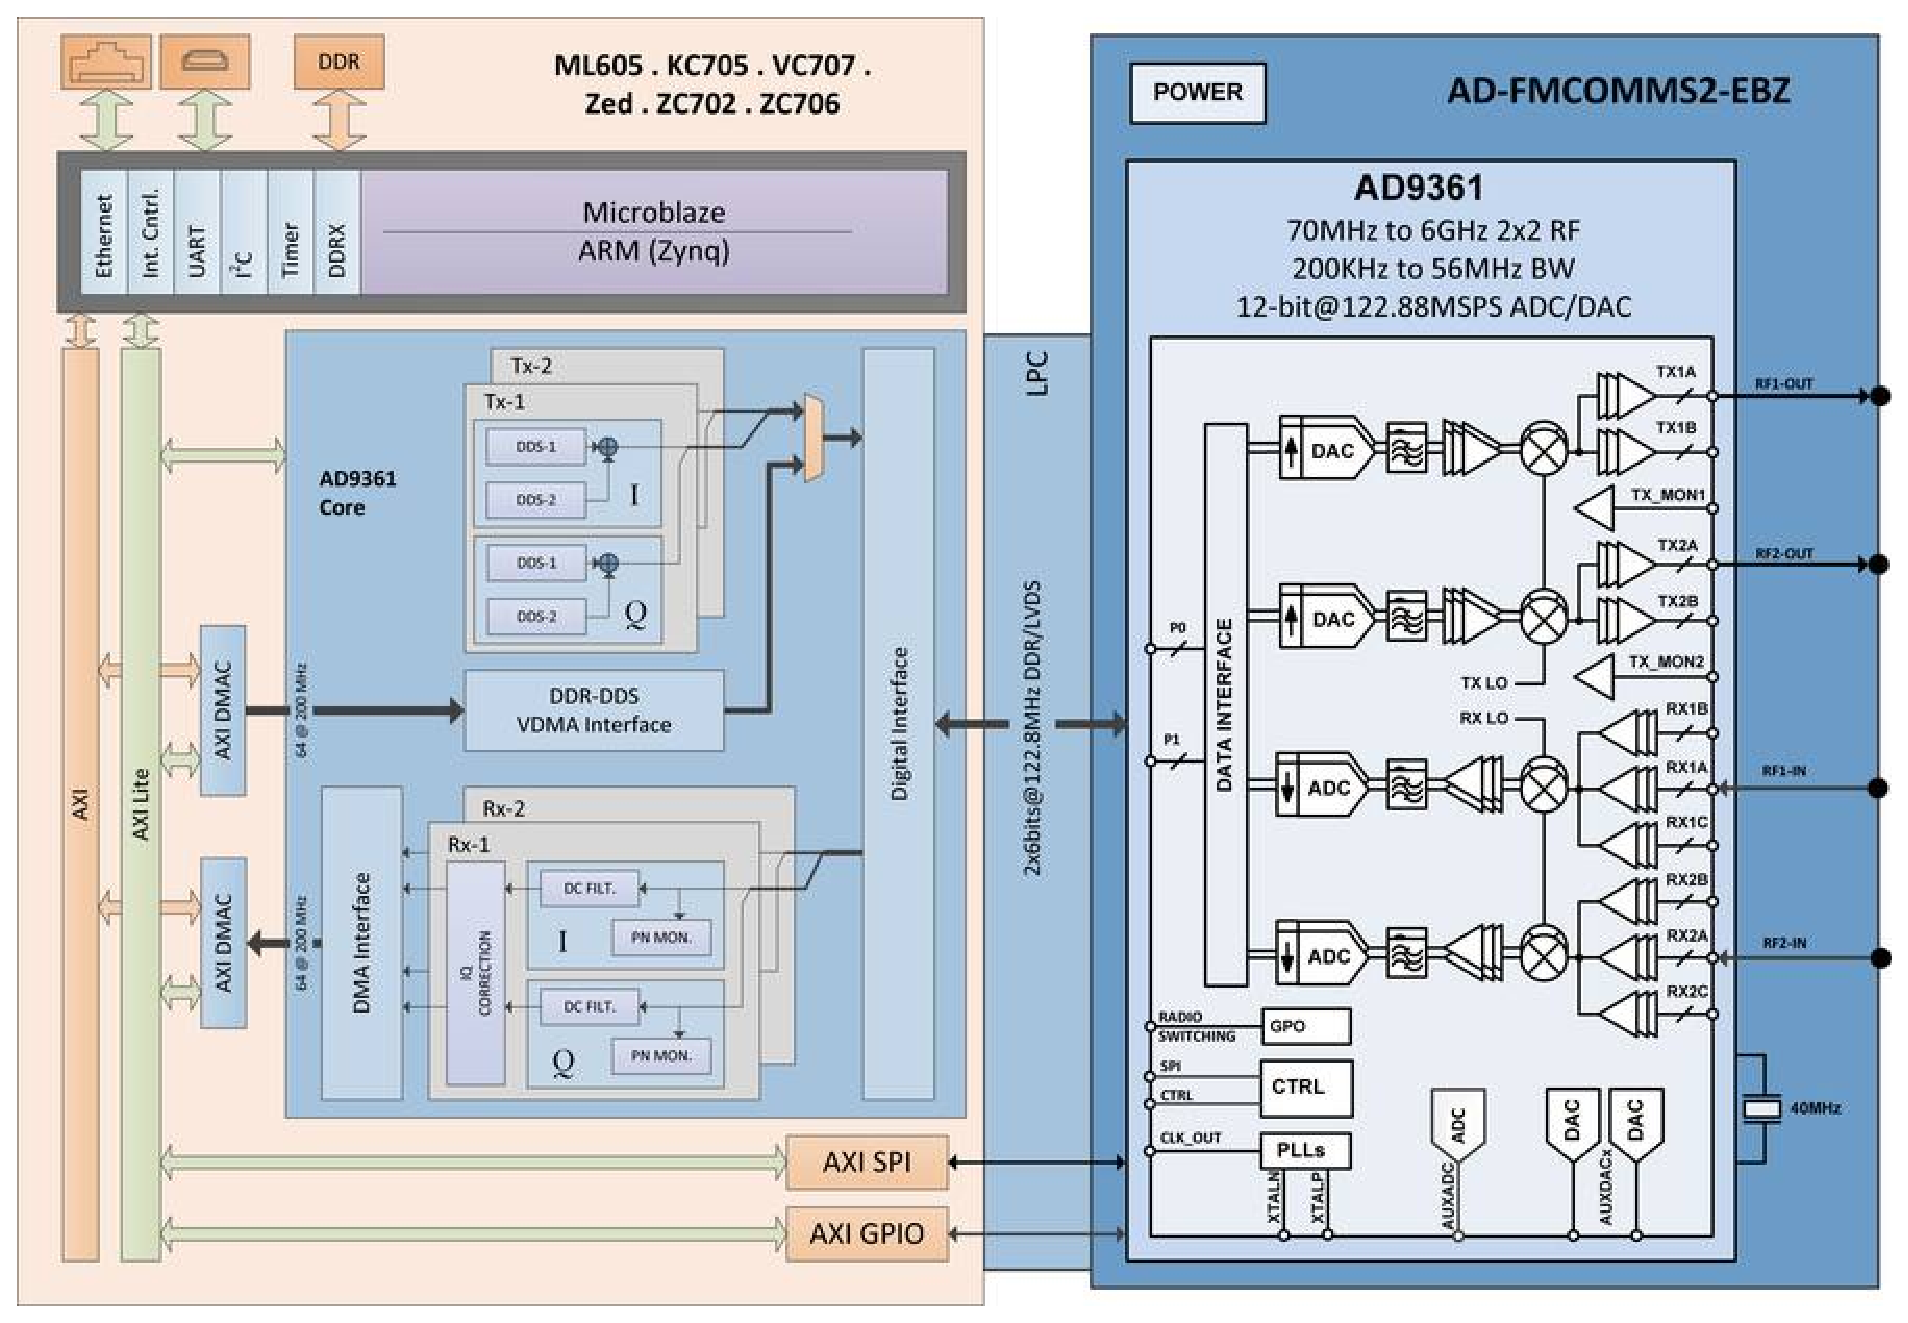
\includegraphics[width=0.65\textwidth]{./figures/fmcomms2_bd}
    \caption{ FMComms2 and FPGA Block Diagram
    \label{fig:fmcommbd}}
\end{figure}



\begin{description}
	\item[Receive] \hfill \\
	\begin{itemize}
		\item Support up to 2 direct conversion RF receiver channels.
		\item Fully integrated frequency synthesizers (including loop filter).
		\item Data path consists in LNA, Demodulator, LPF, ADC and digital filters.
		\item \textit{AGC:} quadrature calibration and DC offset calibration.
		\item \textit{NF:} 2.5 dB at 1Ghz.
		\item \textit{ADC:} Continuous time sigma-delta ( $\Sigma - \Delta$), 640 MSPS.
		\item \textit{Digital FIlter:} 128 COmplex taps with decimation between 2 and 48.
		\item \textit{Gain:} 1dB step size, 80 dB analog Range, 30 db digital range (post ADC scaling).
		\item On-chip sensor for temperature corrected RSSI.
	\end{itemize}

	\item[Transmit] \hfill \\
\begin{itemize}
		\item Supports up to 2 direct conversion RF transmit channels.
		\item Fully integrated frequency synthesizers (including loop filter).
\item Data path consists of digital filters, DAC and modulators.
		\item \textit{Digital FIlter:} 128 complex taps with interpolation between 2 and 48.
		\item \textit{Gain:} 0.5 dB step size, 86 dB range.
		\item \textit{ADC:} 340 MSPS.
	\end{itemize}

	\item[Clocking] \hfill \\
		The FMComms2 board has a integrated crystal oscillator of 40 Mhz and has a SMA input for external clock input.

	\item[Control/Monitor] \hfill \\
		The board allows real time control and monitoring via dedicated pins, such pins functionality are programmable. The control and monitor programming configuration is specified in the ad9361 section \cite{sec:ad9361}.

\end{description}

\section{Basic Mathematical Background}

\subsection{Complex Modulation}

\begin{eqnarray}
	I = sin(\omega \times t)\\
	Q = cos(\omega \times t)
\end{eqnarray}

\begin{equation}
	cos(\omega \times t) = sin(\frac{\pi}{2} - (\omega \times t))
\end{equation}

then:

\begin{eqnarray}
	I = sin(\omega \times t)\\
	Q = sin(\frac{\pi}{2} - (\omega \times t))
\end{eqnarray}

These are the two signals coming out of the DAC, two sine waves, phase offset from each other, wich is called IQ.

\subsection{Basic Modulation Mathematics}

Start to modulating signal from a amplitude perspective:

\begin{eqnarray}
LO_I = A_x cos(k)\\
LO_Q = B_x sin(k)
\end{eqnarray}

We still have the carrier:

\begin{equation}
LO_I = cos(\omega) ; LO_Q = sin(\omega)
\end{equation}

Will result:

\begin{eqnarray}
LO_I \times I = A_x cos(k) \times sin(\omega)\\
LO_Q \times I = B_x sin(k) \times cos(\omega)
\end{eqnarray}


That gives the output:

\begin{equation}
x(t)=A_x cos(k)\times sin(\omega)+ B_x sin(k)\times cos(\omega)
\end{equation}

This does not match with any trigonometrical identities and it is easier to use Euler\'s formula:

\begin{eqnarray}
sin(x)=(\frac{1}{2}e^{-jx} - \frac{1}{2}e^{jx})\\
cos(x)=(\frac{1}{2}e^{-jx} + \frac{1}{2}e^{jx})
\end{eqnarray}

Therefore:

\begin{equation}
x(t)=A_x (\frac{1}{2}e^{-jk} + \frac{1}{2}e^{jk})\times (\frac{1}{2}e^{-j\omega} - \frac{1}{2}e^{j\omega})+ B_x (\frac{1}{2}e^{-jk} - \frac{1}{2}e^{jk})\times (\frac{1}{2}e^{-j\omega} + \frac{1}{2}e^{j\omega})
\end{equation}

\begin{equation}
x(t)=\frac{A}{2} (e^{-jk} + e^{jk})\times (e^{-j\omega} - e^{j\omega})+ \frac{B}{2} (e^{-jk} - e^{jk})\times (e^{-j\omega} + e^{j\omega})
\end{equation}

If we expand we get:

\begin{equation}
x(t)=\frac{1}{2} ((Ae^{-jk-j\omega} + Ae^{jk-j\omega} - Ae^{-jk+j\omega} - Ae^{jk+j\omega}) + (Be^{-jk-j\omega} - Be^{jk-j\omega} - Be^{-jk+j\omega} + Be^{jk+j\omega}))
\end{equation}


And then:

\begin{equation}
x(t)=\frac{1}{2} ((A+B)e^{-jk-j\omega} + (A-B)e^{jk-j\omega} - (A-B)e^{-jk+j\omega} - (A+B)e^{jk+j\omega})
\end{equation}

It is possible to rearrange as:

\begin{equation}
x(t)=\frac{1}{2} \times ((A+B)(e^{-jk-j\omega} - e^{jk+j\omega}) + (A-B)(e^{jk-j\omega} - e^{-jk+j\omega}))
\end{equation}

And then:

\begin{equation}
x(t)=(\frac{A+B}{2} )(sin(k+\omega)) + (\frac{A-B}{2} )(sin(k-\omega))
\end{equation}

If this due to amplitude mismatch, this creates an image on the other side of the local oscillator.





%\chapter{Mitigação de Distorção PCI}
\label{sec:mitigacao_pci}

\section{Introdução}

Na seção anterior, apresentou-se o fato de que, devido a um prefixo cíclico insuficiente, surge distorção na saída do canal na forma de interferência inter-simbólica e inter-portadora, as quais foram denominadas como distorção por prefixo cíclico insuficiente (distorção PCI). Esta distorção pode impactar severamente no desempenho de um sistema DMT, motivo pelo qual técnicas que promovam a sua mitigação são extensamente abordadas na literatura.

A grande relação envolvida na mitigação de distorção PCI em sistemas DMT é o compromisso entre o comprimento do prefixo cíclico e a perda que este provoca na taxa de informação. Sabe-se que, para evitar a ocorrência de distorção PCI, o prefixo cíclico deve ser suficiente para cobrir a dispersão causada pelo canal. Por outro lado, sabe-se que o prefixo cíclico diminui a taxa de transmissão de símbolos DMT, já que os símbolos deixam de ter $N$ amostras para ter $\nu + N$ amostras quando o prefixo é adicionado. Assim, ao aumentar o prefixo cíclico, reduz-se a distorção PCI com a desvantagem da diminuição da taxa de transmissão de símbolos. Analogamente, ao diminuir o prefixo cíclico, aumenta-se a taxa de transmissão de símbolos com a desvantagem do aumento da distorção PCI.

Tipicamente, as respostas impulsivas dos canais utilizados em sistemas DMT apresentam grande número de amostras não nulas, devido às elevadas frequências de amostragem. Diante disto, não é prático utilizar valores de prefixo cíclico suficientes para cobrir a dispersão do canal, já que estes reduziriam a taxa de transmissão de símbolos a valores muito baixos. Assim, comumente os sistemas DMT operam com prefixos cíclicos insuficientes, os quais são projetados para cobrir a parte mais significativa da energia proveniente das interferências inter-portadoras e inter-simbólica. Ainda assim, verifica-se que a distorção PCI remanescente degrada significativamente o desempenho do sistema.

A degradação do desempenho e a possibilidade de aumento de taxa de informação com a mitigação de distorção PCI é a motivação para seu estudo. Diversas métodos são conhecidos para este propósito, destacando-se a equalização no domínio do tempo (TEQs) ou encurtamento de canal \cite{chanshort2001,channelshort2003}, equalizadores no domínio da frequência no receptor \cite{Trautmann2002, Park04} e a pré-codificação de símbolos \cite{Malkin08,Cheong98}. Além destas, técnicas como algoritmos iterativos de estimação e mitigação de interferência \cite{stuber1998}, algoritmos de mitigação a partir da exploração de subcanais não utilizados \cite{huang2009}, algoritmos de reserva de subcanais \cite{malkin2007}, dentre outros. Estes métodos, sejam eles baseados em processamento no receptor, no transmissor ou em ambos, introduzem complexidade no sistema, a qual deve ser mantida em um nível aceitável para não contrariar uma das grandes vantagens oferecida por sistemas multiportadora, a baixa complexidade.

Neste trabalho, adota-se a tecnologia de acesso denominada por ``acesso rápido aos terminais do assinante'' (G.fast) \cite{maes2012} como o cenário de interesse para a aplicação das técnicas de mitigação de distorção PCI desenvolvidas. Esta consiste em uma versão de redes DSL em processo de padronização pelo Setor de Normatização das Telecomunicações (ITU-T), a qual busca satisfazer as demandas de altas taxas de bit (até $1$~Gb/s) características dos serviços da quarta geração de banda larga (4GBB) \cite{tno_gfast} utilizando ainda as instalações de cobre (telefônicas) existentes nos domicílios. Para tanto, esta tecnologia adota a solução denominada fibra até a residência (FTTH), na qual procura-se levar a fibra ótica às proximidades das residências, reduzindo o comprimento dos enlaces de cobre (par-trançado) que levam a transmissão do ponto mais próximo onde há fibra até o interior das instalações do usuário.

Nesta tecnologia, a mitigação de distorção PCI apresenta potencial para aumento do desempenho geral das linhas de assinantes contidas em um conjunto de linhas (\textsl{binder}). Nestes sistemas, o operador pode ajustar o comprimento do prefixo cíclico para lidar com a distorção do canal. No entanto, se o \textsl{binder} apresentar linhas com comprimentos diferentes, a linha que possuir maior resposta impulsiva irá impor um prefixo cíclico relativamente grande e, consequentemente, diminuir a taxa de símbolos de todas as linhas, já que, devido a duplexação por divisão de tempo sincronizada (S-TDD), todas devem utilizar o mesmo prefixo cíclico. Neste caso, técnicas que puderem adotar um prefixo cíclico reduzido com custo computacional razoável podem ser factíveis.

Neste trabalho, tem-se como objetivo analisar técnicas de mitigação de distorção PCI em sistemas DMT através da pré-codificação de símbolos no transmissor e equalização no receptor. Estas são extensivamente abordadas para redes sem-fio com sistemas OFDM em \cite{malkin2009}, no qual utiliza-se otimização convexa para pré-codificar os símbolos visando obter a máxima taxa de bits e satisfazer as máximas alocações de potência para cada subcanal. Em conjunto com a pré-codificação, em \cite{malkin2009} é desenvolvido um algoritmo que toma vantagem da alta correlação que existe entre as interferências inter-portadoras e inter-simbólicas no domínio da frequência causadas por tons consecutivos, o que proporciona a diminuição do número de operações necessárias para a pré-codificação. Adicionalmente,  utiliza-se cancelamento de interferência sucessiva (SIC) no receptor para atuar em conjunto com a pré-codificação na mitigação de ICI, o que proporciona ainda menor complexidade.

Em contraste à abordagem de \cite{malkin2009}, a qual é baseada em otimização, neste trabalho serão analisadas técnicas de pré-codificação a partir de soluções fechadas, as quais não necessitam de longas fases de treinamento dedicadas à solução do problema de otimização\footnote{O problema de otimização referido consiste em calcular a matriz de pré-codificação ótima para a maximização da taxa de bits, tendo como restrição os limites de potência.}. Nesta capítulo, serão apresentadas as estruturas fundamentais de pré-codificação de ICI no transmissor (Seção \ref{sec:prec_ICI}), equalização de ISI no receptor (Seção \ref{sec:isi_equalization}) e pré-codificação conjunta de ICI e ISI no transmissor (Seção \ref{sec:precodificacao_isi_ici}). Sequencialmente, apresenta-se na Seção \ref{sec:complexidade_precodificacao} uma análise da complexidade dos algoritmos desenvolvidos. Finalmente, simula-se o desempenho de sistemas com a utilização da pré-codificação e equalização na Seção \ref{sec:ici_isi_pre_sim}. 

É importante observar que, no desenvolvimento apresentado, a complexidade dos algoritmos  será relativamente alta e a alteração de potência no símbolo introduzida pelo processo de pré-codificação será solucionada de maneira pouco elaborada, já que as alternativas para redução de complexidade e controle de potência serão apresentadas em detalhes no Capítulo \ref{sec:power_control}. 

\section{Pré-codificação de Símbolos para Mitigar ICI}
\label{sec:prec_ICI}

Inicialmente, será considerada a técnica de pré-codificação de símbolos para mitigação de interferência inter-portadora (ICI) no símbolo recebido. Esta técnica consiste em introduzir pré-distorção no símbolo a ser transmitido, de maneira que, quando efetivamente transmitido, esta seja eliminada pela distorção natural do canal, restando ao receptor o símbolo desejado sem interferência inter-portadora.

\begin{figure}[htbp]
\centering
\includegraphics[width=1\textwidth]{./figs/cadeia_dmt_precoder}
\caption{Cadeia DMT com a inclusção do pré-codificador.
\label{fig:cadeia_dmt_prec}}
\end{figure}

Par tanto, introduz-se um bloco pré-codificador de símbolos na cadeia DMT original (Figura \ref{fig:cadeia_ofdm}), o qual tem como finalidade transformar o símbolo DMT original, obtido a partir do mapeador QAM, em um símbolo pré-codificado. Neste caso, devido ao fato de que o pré-codificador tem como entrada o símbolo DMT no domínio da frequência, diz-se que o pré-codificador atua no domínio da frequência. A cadeia DMT resultante está apresentada na Figura \ref{fig:cadeia_dmt_prec}, na qual destaca-se o pré-codificador entre o mapeador de constelações e o operador IFFT. 

O pré-codificador consiste em uma matriz $\mathbf{W}$, a qual multiplica o símbolo DMT (vetor $\mathbf{X}$), resultando no símbolo pré-codificado $\tilde{\mathbf{X}}$. Assim, visando a chegada do símbolo original ($\mathbf{X}$) no receptor, transmite-se o símbolo pré-codificado $\tilde{\mathbf{X}}$, como será visto no desenvolvimento que segue. Os vetores de entrada e saída do bloco pré-codificador estão destacados no esquema da Figura \ref{fig:pre_codificador}. 

\begin{figure}[htbp]
\centering
\tikzstyle{box} = [rectangle, draw, text width=5em, text centered, minimum height=5em]
\tikzstyle{boxs} = [rectangle, draw, text width=5em, text centered, minimum height=5em, color=red]
\tikzstyle{line} = [draw, -latex']
\begin{tikzpicture}[node distance = 2cm, auto]
\node [] (DMTs) [] {\text{\parbox{3 cm}{\centering Símbolo DMT Transmitido}}};
\node [box] (Prec) [right of=DMTs,xshift = 8em] {Pré-codificador};
\node [] (IFFT) [right of=Prec, xshift=8em] {\text{\parbox{3 cm}{\centering Símbolo pré-codificado}}};
\path [line] (DMTs) -- node[] {$\mathbf{X}$}  (Prec);
\path [line] (Prec) -- node[] {$\tilde{\mathbf{X}} = \mathbf{WX}$} (IFFT);
\end{tikzpicture}
\caption{Esquema de pré-codificação.
\label{fig:pre_codificador}}
\end{figure}

É importante destacar que a matriz de pré-codificação $\mathbf{W}$ é função do canal, isto é, necessita da resposta impulsiva do canal e do conhecimento do atraso ($n_0$) para ser construída. Isto é esperado, já que o pré-codificador precisa conhecer a distorção introduzida pelo canal para poder promover a sua mitigação. Assim, é necessário que o transmissor tenha a informação do canal para realizar a pré-codificação, o que torna necessário a estimação de canal.

Por ora, assume-se que o transmissor detém perfeito conhecimento do canal. Na prática, este conhecimento perfeito não é facilmente garantido \cite{malkin2009}. No entanto, em sistemas de comunicação no qual o canal não apresenta variações rápidas, como é o caso de sistemas de comunicação cabeados, é possível obter a estimativa do canal com maior confiabilidade. 

\subsection{Modelamento do Símbolo Recebido no Domínio da Frequência}

Para iniciar o desenvolvimento do pré-codificador, tem-se como objetivo conhecer a transformada discreta de Fourier do conteúdo de ISI e ICI no domínio do tempo introduzido pelo símbolo transmitido. Em outras palavras, deseja-se expressar a DFT da ISI ($\mathbf{Y}_\text{ISI}$) e a DFT da ICI ($\mathbf{Y}_\text{ICI}$) conforme as expressões abaixo:
\begin{align}
\mathbf{Y}_\text{ISI}^{(i)} &=\mathbf{ T_\text{ISI}}\mathbf{X^{(i-1)}} \label{eq:ISI_Tisi}\\
\mathbf{Y}_\text{ICI}^{(i)} &=\mathbf{ T_\text{ICI}\mathbf{X^{(i)}}} \label{eq:ISI_Tici}
\end{align}
onde $\mathbf{ T_\text{ISI}}$ e $\mathbf{ T_\text{ICI}}$ são as matrizes que transformam linearmente os símbolos no domínio da frequência $\mathbf{X}$ em suas ISIs e ICIs no domínio da frequência. 

Para expressar dessa maneira, utiliza-se as representações matriciais da ISI e ICI no domínio do tempo, apresentadas nas Equações \ref{eq:ISI_matrix_rep} e \ref{eq:ICI_matrix_rep_vec}, as quais são repetidas abaixo por conveniência:
\begin{align}
\mathbf{y}_\text{ISI}^{(i)} &= \mathbf{ H_\text{ISI}} \mathbf{x}^{(i-1)}[((n + n_0))_N] \nonumber\\
\mathbf{y}_\text{ICI}^{(i)} &= \mathbf{ H_\text{ICI}} \mathbf{x}^{(i)}[((n + n_0))_N] \nonumber
\end{align}
onde $((n + n_0))_N$ denota o deslocamento circular de $n_0$ amostras dentre as $N$ amostras do símbolo.

Em seguida, calcula-se as DFTs destes vetores de ISI e ICI segundo a definição da Equação \ref{eq:m_dft}:
\begin{align}
\mathbf{Y}_\text{ISI}^{(i)} &= \mathbf{Q} \mathbf{ H_\text{ISI}} \mathbf{x}^{(i-1)}[((n + n_0))_N]
\label{eq:partial_ISI_DFT}\\
\mathbf{Y}_\text{ICI}^{(i)} &= \mathbf{Q} \mathbf{ H_\text{ICI}} \mathbf{x}^{(i)}[((n + n_0))_N] 
\label{eq:partial_ICI_DFT}
\end{align}

Adicionalmente, observa-se que os símbolos no domínio do tempo com deslocamento circular podem ser expressos como a IDFT de suas representações no domínio da frequência, isto é, a IDFT de suas DFTs. Para tanto, considera-se a propriedade do deslocamento circular no domínio do tempo correspondente a multiplicação dos subsímbolos componentes do vetor DFT por exponenciais complexas, conforme abaixo \cite{dspambardar}:

$$ \mathbf{x}[((n + n_0))_N] \leftrightarrow X_ke^{j2\pi k n_0/N} $$
onde $\leftrightarrow$ denota a correspondência entre o domínio do tempo (lado esquerdo) e o domínio da frequência (lado direito).


Portanto, utilizando a definição de IDFT da Equação \ref{eq:m_idft}, expressa-se o vetor $ \mathbf{x}[((n + n_0))_N]$ como:
\begin{align}
\mathbf{x}^{(i)}[((n + n_0))_N] &=  \mathbf{Q}^\text{H} \mathbf{\Theta_{n_0} \mathbf{X^{(i)}}}  
\label{eq:x_circ_shift_time}
\end{align}
onde $\mathbf{\Theta}_{n_0}$ é uma matriz diagonal, função do atraso $n_0$, cujos elementos correspondem ao deslocamento de fase em cada subcanal, originados pelo deslocamento circular do símbolo no domínio do tempo. Os elementos na diagonal principal em cada linha $k$ da matriz são as exponenciais complexas $e^{j2\pi k n_0/N}$, isto é, $\mathbf{\Theta}(n_0)$ é dada por:
\begin{align}
\mathbf{\Theta(n_0)} = \left[ \begin{array}{ccccc}
1 & 0 & 0 & \cdots & 0\\
0 & e^{-j\frac{2\pi n_0}{N}} & 0 & \cdots & 0\\
\vdots & \vdots & \ddots & \vdots & \vdots\\
0 & 0 & 0 & e^{-j\frac{2\pi n_0}{N}(N-2)} & 0\\
0 & 0 & 0 & \cdots & e^{-j\frac{2\pi n_0}{N}(N-1)}\\
\end{array} \right]
\end{align}

Assim, substituindo a Equação \ref{eq:x_circ_shift_time} nas Equações \ref{eq:partial_ISI_DFT} e \ref{eq:partial_ICI_DFT}, resulta em:
\begin{align}
\mathbf{Y_\text{ISI}^{(i)}} &=  \mathbf{Q} \mathbf{ H_\text{ISI}} \mathbf{Q}^\text{H} \mathbf{\Theta}_{n_0} \mathbf{X}^{(i-1)}
\label{eq:partial_ISI_DFT2}\\
\mathbf{Y_\text{ICI}^{(i)}} &=  \mathbf{Q} \mathbf{ H_\text{ISI}} \mathbf{Q}^\text{H} \mathbf{\Theta_{n_0} \mathbf{X^{(i)}}}
\label{eq:partial_ICI_DFT2}
\end{align}

Portanto, conclui-se que as matrizes $\mathbf{ T_\text{ISI}}$ e $\mathbf{ T_\text{ICI}}$ das Equações \ref{eq:ISI_Tisi} e \ref{eq:ISI_Tici} são dadas, respectivamente, por:
\begin{align}
\mathbf{ T_\text{ISI}} &= \mathbf{Q} \mathbf{ H_\text{ISI}} \mathbf{Q}^\text{H} \mathbf{\Theta_{n_0}}\\
\mathbf{ T_\text{ICI}} &= \mathbf{Q} \mathbf{ H_\text{ICI}} \mathbf{Q}^\text{H} \mathbf{\Theta_{n_0}}
\label{eq:tici_definition}
\end{align}

Na sequência, similarmente à Equação \ref{eq:yideal_yisi_ici}, divide-se o símbolo recebido no domínio da frequência em três parcelas: a parte ideal, a qual seria recebida se não houvesse distorção PCI; a parte correspondente à ISI e a parte correspondente à ICI.
\begin{align}
\mathbf{Y}^{(i)}= \mathbf{Y}_\text{Ideal}^{(i)} + \mathbf{Y}_\text{ISI}^{(i)} + \mathbf{Y}_\text{ICI}^{(i)}
\label{eq:rx_symbol_freq_domain}
\end{align}

Substituindo as Equações \ref{eq:ISI_Tisi} e  \ref{eq:ISI_Tici} na equação acima, resulta na seguinte representação para o $i$-ésimo símbolo recebido no domínio da frequência:
\begin{align}
\mathbf{Y}^{(i)} &=  \mathbf{Y}_\text{Ideal}^{(i)} + \mathbf{ T_\text{ISI}} \mathbf{X^{(i-1)}} + \mathbf{ T_\text{ICI} \mathbf{X^{(i)}}}\nonumber
\end{align}
onde a parcela $\mathbf{Y}_\text{Ideal}^{(i)}$ é obtida a partir da DFT da Equação \ref{eq:y_ideal}, conforme abaixo:
\begin{align}
\mathbf{Y}_\text{Ideal}^{(i)} = \mathbf{Q} \mathbf{y}_\text{Ideal}^{(i)}  = \mathbf{Q} \mathbf{ \tilde{H} } \mathbf{x}^{(i)}[((n + n_0))_N] = \mathbf{Q} \mathbf{ \tilde{H} } \mathbf{Q}^\text{H} \mathbf{\Theta_{n_0} \mathbf{X^{(i)}}}
\label{eq:y_ideal_freq_domain}  
\end{align}
Pode-se demonstrar que os vetores base da matriz DFT diagonalizam a matriz circulante \cite{malkin2009}, já que os autovetores da matriz circulante correspondem aos vetores linearmente independentes que formam as bases da matriz DFT. Portanto, a decomposição em autovalores da matriz circulante $\tilde{\mathbf{H}}$ resulta em:
\begin{align}
\tilde{\mathbf{H}} =  \mathbf{Q}^H \tilde{\mathbf{\Lambda}} \mathbf{Q}
\label{eq:hcirc_diag}
\end{align}
onde $\tilde{\mathbf{\Lambda}}$ é uma matriz diagonal cujos elementos da diagonal principal correspondem à DFT da resposta impulsiva do canal e são os autovalores de $\tilde{\mathbf{H}}$ \cite{gray2006}.

Isolando a matriz de ganhos do canal $\tilde{\mathbf{\Lambda}}$ na Equação \ref{eq:hcirc_diag} e considerando que $\mathbf{Q}$ é uma matriz unitária ($\mathbf{Q}\mathbf{Q}^H=1$), obtém-se:
\begin{align}
\tilde{\mathbf{\Lambda}} = \mathbf{Q}\tilde{\mathbf{H}}Q^H 
\label{eq:h_gain_diag}
\end{align}

Substituindo a Equação \ref{eq:h_gain_diag} na Equação \ref{eq:y_ideal_freq_domain}, resulta em:
\begin{align}
\mathbf{Y}_\text{Ideal}^{(i)} = \tilde{\mathbf{\Lambda}} \mathbf{\Theta_{n_0} \mathbf{X^{(i)}}}
\end{align}

Pode-se, no entanto, agrupar o produto $\tilde{\mathbf{\Lambda}}\mathbf{\Theta}_{n_0}$ em somente uma matriz, a qual será denominada $\mathbf{\Lambda}$:
\begin{align}
\mathbf{\Lambda}  = \tilde{\mathbf{\Lambda}}\mathbf{\Theta}_{n_0} = \mathbf{Q}\tilde{\mathbf{H}}\mathbf{Q}^H\mathbf{\Theta}_{n_0}
\label{eq:lambda_definition}
\end{align}

Neste caso, o vetor $\mathbf{Y}_\text{Ideal}^{(i)}$ pode ser expresso como:
\begin{align}
\mathbf{Y}_\text{Ideal}^{(i)} = \mathbf{\Lambda \mathbf{X^{(i)}}}
\end{align}

Finalmente, substituindo a expressão acima na Equação \ref{eq:rx_symbol_freq_domain}, obtém-se a expressão que modela o símbolo recebido no domínio da frequência em função dos símbolos presente e precedente:
\begin{align}
\mathbf{Y}^{(i)} &=\left(\mathbf{\Lambda} + \mathbf{ T_\text{ICI}}\right) \mathbf{X^{(i)}} + \mathbf{ T_\text{ISI}} \mathbf{X^{(i-1)}}\nonumber\\
\mathbf{Y}^{(i)} &= \mathbf{A} \mathbf{X^{(i)}} + \mathbf{ T_\text{ISI}} \mathbf{X^{(i-1)}}
\label{eq:model_y_rx_freq_domain}
\end{align}
onde $\mathbf{A}=\left(\mathbf{\Lambda} + \mathbf{ T_\text{ICI}}\right)$, isto é, $\mathbf{A}$ é a matriz com os ganhos dos subcanais diretos e os ganhos de \textsl{crosstalk} entre os subcanais (devido à ICI).

No entanto, ao considerar o pré-codificador para mitigar somente a ICI, assume-se que a ISI seja completamente eliminada no receptor, como em  \cite{Malkin08,Park04}. Por isso, pode-se modelar o símbolo recebido como:
\begin{align}
\mathbf{Y}^{(i)} &= \mathbf{A} \mathbf{X^{(i)}}
\label{eq:model_y_rx_freq_domain_ici}
\end{align}

\subsection{Pré-codificação de ICI}

A partir da expressão do símbolo recebido afetado por distorção PCI no domínio da frequência, apresentada na Equação \ref{eq:model_y_rx_freq_domain_ici}, é direto demonstrar que é possível escolher o símbolo a ser transmitido $\tilde{X}$ de maneira que o símbolo recebido seja o símbolo ideal, isto é:
\begin{align}
\mathbf{Y}^{(i)} &= \mathbf{Y}_\text{Ideal}^{(i)} = \mathbf{\Lambda} \mathbf{X^{(i)}} \nonumber
\end{align}

Para tanto, é necessário que o símbolo pré-codificado seja dado por:
\begin{align}
\mathbf{\tilde{X}}^{(i)} = \mathbf{A}^{-1}\mathbf{\Lambda} \mathbf{X^{(i)}}
\label{eq:precoder_ici_isi}
\end{align}
na qual assume-se que a matriz $\mathbf{A}$ seja invertível.

Neste caso, como o símbolo pré-codificado é o produto entre a matriz pré-codificadora ($\mathbf{W}$) e o símbolo original ($\mathbf{X}$), conclui-se que a matriz pré-codificadora é dada por:
\begin{align}
\mathbf{W} =  \mathbf{A}^{-1}\mathbf{\Lambda}
\label{eq:prec_no_norm}
\end{align}

\subsection{Considerações sobre Potência}

Essencialmente, este pré-codificador força o canal real a não apresentar \textsl{crosstalk} entre os subcanais, ao providenciar a diagonalização da matriz do canal real ($\mathbf{A}$). Este pré-codificador é similar a estrutura de diagonalização do canal apresentada para eliminação de \textsl{crosstalk} entre as linhas de transmissão em \cite{Cendrillon07}, na qual, ao invés de eliminar o \textsl{crosstalk} entre os subcanais (ICI), elimina-se o \textsl{crosstalk} entre os usuários cujos canais estão em um mesmo \textsl{binder}. 

Contudo, a eliminação de \textsl{crosstalk} entre os subcanais pode demandar aumentos de potência de transmissão, como um preço a ser pago para forçar a diagonalização do canal. A operação de pré-codificação altera a distribuição de potência do símbolo transmitido, podendo esta ultrapassar os limites de potência estabelecidos para cada subcanal (máscara de potência). Para visualizar este efeito, observa-se que o $k$-ésimo subsímbolo do símbolo DMT pré-codificado é dado por:
\begin{align}
\tilde{X}_k &= \mathbf{w}_k \mathbf{X}\nonumber\\
&= \sum \limits_{m=0}^{N-1} w_{k,m} X_m
\label{eq:xtilde_innerp}
\end{align}
onde o $\mathbf{w}_k $ é o vetor-linha com os elementos da $k$-ésima linha de $\mathbf{W}$ e $w_{k,m}$ é o elemento na $k$-ésima linha e $m$-ésima coluna de $\mathbf{W}$, isto é, $\mathbf{w}_k  = \left[ w_{k,0}, w_{k,1}, \cdots, w_{k,N-1} \right]$.

Sequencialmente, nota-se que a densidade espectral de potência média ($\tilde{s}_k$) no $k$-ésimo subcanal pré-codificado é dada por\footnote{A densidade espectral de potência apresentada corresponde à definição de DFT adotada na Equação \ref{eq:q_matrix}.}:
\begin{align}
\tilde{s}_k \stackrel{\Delta}{=} \frac{E \{ \left| \tilde{X}_k \right|^2 \}}{N}
\label{eq:psd_definition}
\end{align}
onde o operador $E\{ \cdot \}$ denota o valor esperado.

Substituindo $\tilde{X}_k$ da Equação \ref{eq:xtilde_innerp}, obtém-se:
\begin{align}
\tilde{s}_k &=  \frac{E \left\{ \left| \sum \limits_{m=0}^{N-1} w_{k,m} X_m \right|^2 \right\} }{N}
\end{align}

Contudo, devido ao valor absoluto de um somatório ser menor ou igual o somatório dos valores absolutos (propriedade da desigualdade triangular), a PSD no subcanal $k$ torna-se:
\begin{align}
\tilde{s}_k &\leq  \frac{E \left\{  \sum \limits_{m=0}^{N-1} \left|w_{k,m} X_m \right|^2 \right\} }{N} \nonumber\\
&\leq  \frac{E \left\{  \sum \limits_{m=0}^{N-1} \left|w_{k,m} \right|^2 \left|X_m \right|^2 \right\} }{N} \nonumber
\end{align}

Adicionalmente, dado que a matriz de pré-codificação $\mathbf{W}$ não é aleatória, o valor esperado aplica-se somente ao termo $X_m$. Neste caso, a expressão torna-se:
\begin{align}
\tilde{s}_k  &\leq  \frac{\sum \limits_{m=0}^{N-1} \left|w_{k,m} \right|^2 E \left\{  \left|X_m \right|^2 \right\} }{N} \nonumber
\end{align}

Substituindo a definição de PSD da Equação \ref{eq:psd_definition} no termo $\frac{E \left\{  \left|X_m \right|^2 \right\} }{N}$, tem-se:
\begin{align}
\tilde{s}_k  &\leq  \sum \limits_{m=0}^{N-1} \left|w_{k,m} \right|^2 s_m \nonumber
\end{align}

Finalmente, considera-se que a PSD é distribuída igualmente entre os subcanais, o que implica que o termo correspondente a PSD do subsímbolo original no $m$-ésimo subcanal $s_m$ é constante ($s_m = s$). Assim, a expressão torna-se:
\begin{align}
\tilde{s}_k  &\leq  s_k \sum \limits_{m=0}^{N-1} \left|w_{k,m} \right|^2  \nonumber\\
&\leq  s_k \| \mathbf{w}_k \|^2 
\label{eq:psd_bound}
\end{align}

Portanto, vê-se que a PSD no subcanal $k$ devido à transmissão de símbolos pré-codificados é menor ou igual a PSD original (correspondente à transmissão de símbolos não pré-codificados) multiplicada pela norma Euclidiana da $k$-ésima linha da matriz de pré-codificação ($\| \mathbf{w}_k \|$). Portanto, se $\| \mathbf{w}_k \|$ for maior que 1, a PSD dos símbolos pré-codificados pode ultrapassar a PSD original, isto é, $\tilde{s}_k$ pode ser maior que $s_k$. 

Neste caso, a matriz de pré-codificação é normalizada, visando garantir que a PSD do símbolo pré-codificado seja sempre menor que a PSD do símbolo original. Para tanto, introduz-se um escalar $\beta$ na matriz de pré-codificação da Equação \ref{eq:prec_no_norm}, resultado na matriz de pré-codificação normalizada ($\mathbf{W}'$):
\begin{align}
\mathbf{W}' =  \frac{1}{\beta}\mathbf{A}^{-1}\mathbf{\Lambda}
\label{eq:matriz_precoder_beta}
\end{align}

Neste caso, a PSD do $k$-ésimo símbolo pré-codificado passa a ser dada por: 
\begin{align}
\tilde{s}_k &\leq \frac{ \| \mathbf{w}_k \|^2 }{\beta^2}  s_k
\label{eq:psd_bound_norm}
\end{align}

Portanto, para garantir que todos os subsímbolos apresentem PSD abaixo da PSD original, $\beta$ é escolhido como a máxima norma Euclidiana dentre as normas das linhas da matriz $\mathbf{W}$:
\begin{align}
\beta = \max \left\{ \| \mathbf{w}_k \| \right\}
\label{eq:fator_normalizacao}
\end{align}

\section{Equalização de ISI no Receptor}
\label{sec:isi_equalization}

A interferência inter-simbólica (pós-cursora) que afeta o símbolo recebido é, por definição, função somente do canal e do símbolo anterior. Assim, considerando que o receptor conheça o canal e a maneira como este transforma o símbolo anterior em ISI no símbolo atual, é possível que este estime a ISI que afeta o símbolo recebido. Isto é possível devido ao fato de que, no momento do processamento do símbolo atual, o símbolo anterior já é conhecido pelo receptor, pois este foi detectado anteriormente.

Considerando novamente o símbolo $\mathbf{Y}^{(i)}$ recebido como
\begin{align}
\mathbf{Y}^{(i)} &= \mathbf{A} \mathbf{X^{(i)}} + \mathbf{ T_\text{ISI}} \mathbf{X^{(i-1)}} \nonumber
\end{align}
e assumindo que o receptor conheça $\mathbf{X^{(i-1)}}$, conclui-se que é possível mitigar a ISI a partir da eliminação da parcela correspondente a esta, isto é, a eliminação (subtração) de $\mathbf{ T_\text{ISI}} \mathbf{X^{(i-1)}}$.

No entanto, esta implementação pode falhar na perfeita mitigação de ISI, já que o símbolo anterior utilizado para remoção é, na realidade, o símbolo detectado, o qual pode apresentar erros de detecção. Consequentemente, a equalização de ISI está sujeita à propagação de erro, já que o erro na detecção do símbolo implica no erro na remoção de ISI, que por sua vez afeta a probabilidade de erro na detecção do símbolo, e assim por diante. 

Ainda assim, considerando que os sistemas de comunicação são projetados para baixa probabilidade erro, espera-se que o efeito da propagação de erro seja insignificante para o desempenho do sistema. Este será analisado nas simulações apresentadas na Seção \ref{sec:ici_isi_pre_sim}.

\section{Pré-codificação de Símbolos para Mitigação de ICI e ISI}
\label{sec:precodificacao_isi_ici}

A mitigação conjunta de ICI e ISI a partir de pré-codificação de símbolos no transmissor também é possível. Assim, como alternativa à utilização do esquema de pré-codificação de ICI no transmissor e equalização de ISI no receptor, pode-se concentrar no transmissor a complexidade introduzida no sistema.

A formulação da matriz de pré-codificação de ICI e ISI tem um desenvolvimento análogo ao utilizado para a matriz pré-codificadora de ICI. Inicialmente, substitui-se a expressão para o $i$-ésimo símbolo recebido no domínio da frequência ($\mathbf{Y}^{(i)}$), dada pela Equação \ref{eq:model_y_rx_freq_domain}, na condição de que o símbolo real recebido seja o símbolo ideal ($\mathbf{Y}^{(i)} =\mathbf{\Lambda} \mathbf{X^{(i)}}$). A substituição resulta em: 
\begin{align}
\mathbf{A} \mathbf{\tilde{X}}^{(i)} + \mathbf{ T_\text{ISI}} \mathbf{\tilde{X}}^{(i-1)} = \mathbf{\Lambda} \mathbf{X^{(i)}}\nonumber
\end{align}
na qual é importante observar que o símbolo DMT precedente em questão é o símbolo pré-codificado, já que este é o símbolo efetivamente transmitido.

Isolando o símbolo DMT pré-codificado de referência ($\mathbf{\tilde{X}}^{(i)}$) na equação, obtém-se:
\begin{align}
\mathbf{\tilde{X}}^{(i)} = \mathbf{A}^{-1} \left( \mathbf{\Lambda} \mathbf{X^{(i)}} - \mathbf{ T_\text{ISI}} \mathbf{\tilde{X}}^{(i-1)} \right)
\label{eq:precoder_ici_isi}
\end{align}
na qual assume-se que a matriz $\mathbf{A}$ seja invertível.

Neste caso, utilizando a definição da matriz pré-codificadora de ICI ($\mathbf{W}$) em
\ref{eq:prec_no_norm}, pode-se expressar o símbolo pré-codificado a partir de duas matrizes pré-codificadoras:
\begin{align}
\mathbf{\tilde{X}}^{(i)} = \mathbf{W} \mathbf{X^{(i)}} - \mathbf{W}_2 \mathbf{\tilde{X}}^{(i-1)} 
\end{align}
onde $\mathbf{W}_2 = \mathbf{A}^{-1}\mathbf{ T_\text{ISI}}$.

Finalmente, pode-se ainda incluir o fator de normalização na matriz pré-codificadora de ICI, visando satisfazer os limites de potência sob o ponto de vista da parcela $\mathbf{W} \mathbf{X^{(i)}}$. Neste caso, utiliza-se a definição da matriz pré-codificadora normalizada ($\mathbf{W}'$) da Equação~\ref{eq:matriz_precoder_beta}, resultando no seguinte símbolo pré-codificado:
\begin{align}
\mathbf{\tilde{X}}^{(i)} = \mathbf{W}' \mathbf{X^{(i)}} - \mathbf{W}_2 \mathbf{\tilde{X}}^{(i-1)} 
\label{eq:precoder_ici_isi}
\end{align}

\section{Complexidade dos Algoritmos de pré-codificação}
\label{sec:complexidade_precodificacao}

Até o momento, apresentou-se a pré-codificação cuja complexidade será denominada complexidade completa, na qual a matriz pré-codificadora $\mathbf{W}$ (ou $\mathbf{W}'$)  consiste em uma matriz complexa de dimensões $N \times N$. Para esta matriz, a pré-codificação dos símbolos demanda $N^2$ multiplicações escalares complexas e $N(N-1)$ adições escalares complexas, similarmente ao cálculo direto da DFT e IDFT, como apresentado na Seção \ref{sec:complexidade_dft}.

Dado que uma multiplicação escalar complexa requer 4 multiplicações escalares reais e 2 adições escalares reais, enquanto uma adição escalar complexa requer 2 adições escalares reais, o algoritmo requer um total de $4N^2$ multiplicações escalares reais e  $4N^2 - 2N$ adições escalares reais. Este número de operações torna-se bastante elevado à medida que $N$ torna-se considerável. 

Similarmente, o algoritmo de equalização de ISI no receptor requer a multiplicação de uma matriz complexa $N \times N$ ($\mathbf{T}_\text{ISI}$) por um vetor-coluna complexo de $N$ elementos, além de $N$ adições escalares complexas para subtrair o resultado da multiplicação ($\mathbf{T}_\text{ISI} \mathbf{\tilde{X}}^{i-1}$) do símbolo recebido. Portanto, a equalização demanda $4N^2$ multiplicações escalares reais e $4N^2$ adições escalares reais.  

Enquanto isso, a pré-codificação conjunta de ICI e ISI da Equação \ref{eq:precoder_ici_isi} requer 2 multiplicações de matrizes complexas de dimensões $N \times N$ ($\mathbf{W}$ e $\mathbf{W}_2$) por vetores-coluna complexos de N elementos, além de $N$ adições escalares complexas para somar as parcelas. Portanto, o algoritmo necessita realizar $8N^2$ multiplicações escalares reais e $8N^2 - 2N$ adições escalares reais no transmissor.

\begin{table}[htbp]
\centering
\begin{tabular}{ p{5cm} | p{2.5 cm} | p{2.5cm} | p{2.5cm} | p{2.5cm} |}
 & \multicolumn{2}{|c|}{Transmissor} & \multicolumn{2}{|c|}{Receptor}\\
\hline
Algoritmo & Multiplicações escalares reais & Adições escalares reais & Multiplicações escalares reais & Adições escalares reais\\
\hline
Pré-codificação de ICI + Equalização de ISI & $4N^2$ & $4N^2 - 2N$ & $4N^2$ & $4N^2$\\
\hline
Pré-codificação de ICI e ISI & $8N^2$ & $8N^2 - 2N$ & - & - \\
\hline
\end{tabular}
\caption{Complexidade dos algoritmos de pré-codificação. \label{tb:complexidade_dp}}
\end{table}

A complexidade introduzida no transmissor e no receptor pelos algoritmos apresentados está resumida na Tabela \ref{tb:complexidade_dp}. Vê-se que a escolha entre os dois esquemas de mitigação baseia-se na necessidade de distribuir o aumento da complexidade entre transmissor e receptor, ou não. Na seção \ref{sec:power_control}, serão apresentadas alternativas para redução da complexidade destes algoritmos.

\section{Simulações}
\label{sec:ici_isi_pre_sim}

Apresenta-se a simulação dos métodos de mitigação de distorção PCI desenvolvidos nas seções anteriores. Para a simulação, considera-se como canal um cabo par-trançado de alta qualidade (CAT5), típico de instalações DSL, com comprimento de $100$m~, cuja resposta em frequência (apresentada na Figura \ref{fig:ch6_canal_freqresponse}) é conhecida através de medição. Além disto, utiliza-se parâmetros característicos da tecnologia G.fast, destacando-se a largura de banda de aproximadamente $106$~MHz, espaçamento tonal ($\Delta f$) de $51.75$~kHz, $2048$ dimensões complexas ($\bar{N}=2048$ ou $N=4096$), máxima potência de transmissão de $4$~dBm e ruído de fundo com densidade espectral de potência de $-135$~dBm/Hz. 

\begin{figure}[htbp]
\centering
\includegraphics[width=0.95\textwidth]{./figs/simulacao_ch6_canal_freqresponse}
\caption{Espectro de magnitude do canal simulado.
\label{fig:ch6_canal_freqresponse}}
\end{figure}

O algoritmo de carregamento de bits utilizado adota um \textsl{gap} de SNR à capacidade de  $\Gamma = 10.75$, valor típico de instalações DSL atuais \cite{maes2012}, o qual inclui uma margem de ruído de $6$~dB para uma taxa de erro de bits (BER) alvo de $10^{-7}$. Este algoritmo consiste no algoritmo de Levin-Campello para maximização de taxa de bits \cite{campello1999}, o qual implementa a otimização de carregamento discreto de bits (diferentemente das soluções de enchimento com água, as quais resultam em carregamentos reais). Este algortimo baseia-se na análise da energia incremental que cada bit adicional demanda para ser transportado em cada subcanal \cite{ee379c}. Com esta informação, o algoritmo coloca iterativamente cada bit adicional no subcanal que requer menor energia incremental, até que o limite de energia total do símbolo seja satisfeito (ver problema de maximização de taxa de bits na Seção \ref{subsec:bit_loading}). Mais especificamente, o algoritmo implementa os processos de eficientização (\emph{efficientizing}) e estreitamento de energia (\emph{E-tightening}) descritos em \cite{ee379c,campelloisit1998}.

Inicialmente, considera-se a pré-codificação de ICI no transmissor e equalização de ISI no receptor. Para avaliar o desempenho do sistema, compara-se a taxa de bits de informação recebidos sem erro obtida no sistema com o esquema de mitigação e sem, isto é, para um sistema DMT que utiliza os prefixos-cíclicos regularmente. Os prefixos cíclicos utilizados na simulação são de 20, 40, 80, 160 e 320 amostras, os quais correspondem a $0.48\%$, $0.98\%$, $1.95\%$, $3.91\%$ e $7.81\%$ de $N$, respectivamente. Estes obedecem à relação entre taxa de bits e comprimento do prefixo cíclico introduzida na Figura \ref{fig:tradeoff_cp_bitrate}, o que implica na expectativa de maior taxa de bits para o prefixo cíclico de $0.48\%$. 

Para os prefixos cíclicos simulados, a PSD da distorção (soma de ISI e ICI) no símbolo recebido se mantém, na grande maioria dos subcanais, abaixo da PSD ruído de fundo (AWGN). Este comportamento está ilustrado na Figura \ref{fig:ch6_isi_ici_psd}, a qual apresenta a PSD da distorção PCI para cada um dos prefixos cíclicos\footnote{Devido ao elevado número de curvas, opta-se por não identifica-las, o que é irrelevante para o propósito de comparação com a PSD do ruído de fundo.} nos dois casos extremos de potência total de transmissão simulados ($0.2$~dBm e $4$~dBm), além da PSD do AWGN da simulação (em $-135$~dBm/Hz). Estas densidades espectrais de potência da distorção PCI são calculadas de acordo com a demonstração em \cite{perodling2002}. 

\begin{figure}[htbp]
\centering
\includegraphics[width=.95\textwidth]{./figs/simulacao_ch6_isi_ici_psd}
\caption{PSD da distorção PCI em comparação à PSD do AWGN.
\label{fig:ch6_isi_ici_psd}}
\end{figure}

Em relação à pré-codificação, é importante destacar que as linhas dos índices correspondentes aos subcanais das frequências DC e Nyquist ($k=0$ e $k=N/2$) nas matrizes de ISI e ICI no domínio da frequência ($\mathbf{T}_\text{ICI}$ e $\mathbf{T}_\text{ISI}$) são anuladas. Isto se deve ao fato de que estes subcanais não são utilizados para a transmissão, o que implica que suas distorções PCI são irrelevantes. Estas condições são aplicadas visando impedir o crescimento do fator de normalização ($\beta$) da matriz de pré-codificação normalizada (Equação \ref{eq:matriz_precoder_beta}), conforme será visto na Seção \ref{subsec:cond_iniciais}.

A Figura \ref{fig:simulacao_ch6_data_rate_135dbm_noise} apresenta o resultado da taxa de bits corretos recebidos para o sistema com pré-codificação e os sistemas com prefixos cíclicos (sem pré-codificação), além de um limite superior dado pela Equação \ref{eq:chan_capacity_gap} (na qual $\Gamma=10.75$). Nota-se que, como esperado, o desempenho obtido com a utilização de pré-codificação é significativamente superior.

\begin{figure}[htbp]
\centering
\includegraphics[width=1\textwidth]{./figs/simulacao_ch6_data_rate_135dbm_noise}
\caption{Taxa de bits alcançada com a pré-codificação.
\label{fig:simulacao_ch6_data_rate_135dbm_noise}}
\end{figure}

É importante destacar que a simulação cujo resultado está apresentado na Figura \ref{fig:simulacao_ch6_data_rate_135dbm_noise} implementa a equalização de ISI real, a qual, como mencionado na Seção~\ref{sec:isi_equalization}, sujeita-se à propagação de erros. Contudo, observa-se a partir do desempenho apresentado que a propagação de erro é, efetivamente, insignificante para o desempenho do sistema. Este argumento é ainda reforçado ao observar o resultado da simulação que força a remoção perfeita de ISI (sem erros), o qual é exatamente equivalente ao resultado da Figura \ref{fig:simulacao_ch6_data_rate_135dbm_noise}.

Finalmemente, ressalta-se que a pré-codificação de ICI e ISI no transmissor para o mesmo cenário de simulação também resulta exatamente no mesmo desempenho da Figura~\ref{fig:simulacao_ch6_data_rate_135dbm_noise}. É importante reforçar que, neste procedimento, as linhas da matriz $\mathbf{T}_\text{ISI}$ correspondentes aos indices das frequências DC e Nyquist ($k=0$ e $k=N/2$) são anuladas. Isto tipicamente garante que os símbolos pré-codificados (segundo a definição da Equação~\ref{eq:precoder_ici_isi}) respeitem os limites de potência, dado que a matriz mais influente na alteração de potência ($\mathbf{W'}$) já é normalizada.


%\chapter{Altenativas para Controle de Potência e Redução de Complexidade}
\label{sec:power_control}

Os algoritmos de mitigação de distorção por prefixo cíclico insuficiente desenvolvidos no Capítulo \ref{sec:mitigacao_pci} encontram duas grandes restrições para suas aplicabilidades: a alteração da densidade espectral de potência dos símbolos transmitidos e a alta complexidade de processamento. Diante disto, torna-se indispensável analisar criteriosamente técnicas que assegurem a PSD do símbolo pré-codificado no nível desejado e que promovam a redução da complexidade do algoritmo.

A pré-codificação desenvolvida no capítulo anterior tem um bom desempenho quando a inversão do canal não resulta em aumentos significativos de potência. No entanto, para algumas realizações de canais, o aumento de potência resultante da inversão é, de fato, elevado. Neste caso, o fator de normalização (dado pela Equação~\ref{eq:fator_normalizacao}), o qual é utilizado para controlar PSD do símbolo pré-codificado, passa a ser elevado (maior que a unidade), o que implica em uma perda de taxa de bits significativa \cite{malkin2009}, como será visto na Seção \ref{sec:perda_taxa}. Por isso, técnicas que permitam ajustar a matriz de pré-codificação e resultar em um fator de normalização aproximadamente unitário são interessantes para a validez da utilização do algoritmo.

Além da garantia da PSD do símbolo pré-codificado dentro dos limites padronizados, a complexidade do algoritmo precisa ser observada. Sabe-se que o equalizador em frequência (FEQ) de um sistema DMT apresenta somente uma derivação por subcanal, o que implica em $N$ operações de multiplicação escalar complexa por símbolo DMT recebido para efetuar a equalização. Esta complexidade é reduzidíssima quando comparada a complexidade introduzida pelos algoritmos de pré-codificação e equalização, as quais foram resumidas na Tabela \ref{tb:complexidade_dp}. Portanto, é necessário observar cautelosamente a validez de trocar a complexidade reduzida do FEQ pela complexidade elevada do esquema de mitigação de distorção PCI, o qual, além do FEQ, utiliza pré-codificação e equalização de ISI.

Esta seção apresenta técnicas que procuram tornar o fator de normalização global ($\beta$) muito próximo da unidade, a fim de que não haja perdas significativas de taxa de bits. Além disso, apresenta técnicas que promovem a redução do custo computacional da pré-codificação de símbolos.  Inicialmente, apresenta-se na Seção \ref{sec:perda_taxa} uma análise da perda de taxa de bits devido ao fator de normalização. Na sequência, apresenta-se nas Seções \ref{sec:desligamento_subcanais} e \ref{sec:normalizacao_per_tone}, duas técnicas para promover  a redução do fator de normalização: o desligamento de subcanais e a normalização por coluna. Finalmente, apresenta-se nas Seções \ref{sec:hermitian_precoder} e \ref{sec:prec_time_domain} duas estratégias de redução do esforço computacional: a pré-codificação somente dos subsímbolos correspondentes às frequências positivas e a pré-codificação no domínio do tempo.

\section{Perda de Taxa de Bits devido à Normalização}
\label{sec:perda_taxa}

Em um sistema DMT ordinário, no qual não se utiliza a pré-codificação de símbolos, quando o prefixo cíclico é insuficiente (quando há distorção PCI), a razão entre a potência do sinal escalada pelo ganho do canal no $k$-ésimo tom ($\left| H_k \right|$) e a potência do ruído somada a potência da interferência (ISI e ICI) neste tom do símbolo recebido\footnote{A esta razão denomina-se razão sinal ruído mais interferência (SINR).} é dada por:
\begin{align}
\text{SNR}_k = \frac{ \left|H_k \right|^2 s_k }{ \sigma_k^2 + s_\text{ISI}^k + s_\text{ICI}^k }
\label{eq:sinr_rx_symbol}
\end{align}
onde  $s_k$, $s_\text{ISI}^k$, $s_\text{ICI}^k$ e $\sigma_k^2$, são as densidades espectrais de potência do símbolo transmitido, da ISI, da ICI, e do ruído Gaussiano branco, respectivamente, assumindo ISI e ICI como independentes do AWGN.

Enquanto isso, ao utilizar a matriz de pré-codificação normalizada ($\mathbf{W}'$) definida pela Equação~\ref{eq:matriz_precoder_beta} (repetida abaixo por conveniência), assumindo a eliminação perfeita de ISI, tem-se o símbolo recebido como dado pela Equação~\ref{eq:rx_symbol_beta}.
\begin{align}
\mathbf{W}' =  \frac{1}{\beta}\mathbf{A}^{-1}\mathbf{\Lambda}
\tag{\ref{eq:matriz_precoder_beta}}
\end{align}
\begin{align}
\mathbf{Y}^{(i)} =\frac{1}{\beta}\mathbf{\Lambda} X^{(i)}
\label{eq:rx_symbol_beta}
\end{align}

Neste caso, a SNR do símbolo recebido é dada por:
\begin{align}
\text{SNR}_k= \frac{\left|H_k \right|^2 \cdot s_k}{ \beta^2 \sigma_k^2 }
\label{eq:snr_rx_symbol}
\end{align}

Nota-se que, ao utilizar a pré-codificação, a SNR do símbolo recebido é alterada por um fator $1/\beta^2$. Em decibéis, a SNR do símbolo recebido no $k$-ésimo tom é dada por:
\begin{align}
\text{SNR}_k &= 10\log \left( \frac{\left|H_k \right|^2 \cdot s_k}{ \beta^2 \cdot \sigma_k^2 } \right) \nonumber\\
&= 10\log \left( \frac{\left|H_k \right|^2 \cdot s_k}{ \sigma_k^2 } \right) - 10 \log \left( \beta^2\right)
\end{align}

Portanto, nota-se que o fator de normalização $\beta$ introduz uma diferença de $ - 20\log(\beta)$ dB na SNR de todos os tons, a qual implica em uma perda de SNR se $\beta$ for maior que a unidade ($\beta > 1$). Esta alteração na SNR modifica a taxa de bits alcançável para o sistema, conforme a definição da Equação~\ref{eq:chan_capacity_gap}.  Assumindo um \textsl{gap} de SNR para a capacidade $\Gamma$, o limite superior da taxa de bits passa a ser dado por:
\begin{align}
\bar{b} = \sum \limits_{k=0}^{N-1} \log \left[1 + \frac{ \left|H_k \right|^2 \cdot s_k }{\beta^2  \Gamma  \sigma_k^2 } \right] \Delta f
\end{align}
onde $\Delta f$ é o espaçamento tonal.

Logo, conclui-se que, quando o fator de normalização ($\beta$) é maior que a unidade, a taxa de bits alcançável para o sistema é reduzida. Portanto, existe uma relação de compromisso entre as SNRs da Equação~\ref{eq:sinr_rx_symbol} e da Equação~\ref{eq:snr_rx_symbol}. Para alguns canais, a mitigação da distorção PCI respeitando a máscara de PSD resulta em um fator de normalização muito maior que 1, o que torna a SNR da Equação~\ref{eq:snr_rx_symbol} (sistema com pré-codificação) menor que a SNR original da Equação~\ref{eq:sinr_rx_symbol} (sistema com distorção PCI).

Ainda assim, deve-se observar que uma SNR mais baixa com a pré-codificação não necessariamente implica em um desempenho pior para o sistema, em comparação ao sistema DMT sem pré-codificação. Isto se deve ao fato de que o sistema sem pré-codificação necessita enviar $\nu$  amostras a mais por símbolo para transmistir a mesma informação, já que envia o prefixo cíclico.

\section{Desligamento de Subcanais}
\label{sec:desligamento_subcanais}

O fator de normalização da matriz de pré-codificação é definido como a máxima norma Euclidiana dentre as normas das linhas da matriz de pré-codificação não normalizada, conforme a Equação~\ref{eq:fator_normalizacao}. Cada uma destas normas tem uma correspondência com a potência necessária para eliminar a distorção PCI no tom de indíce correspondente. Isto foi evidenciado na Equação~\ref{eq:psd_bound} (repetida abaixo), a qual determina o limite superior da PSD no $k$-ésimo tom do símbolo pré-codificado (sem utilização do fator de normalização). 
\begin{align}
\tilde{s}_k  &\leq s_k \| \mathbf{w}_k \|^2 
\tag{\ref{eq:psd_bound}}
\end{align}

Nota-se, na Equação~\ref{eq:psd_bound}, que a norma Euclidiana da $k$-ésima linha da matriz de pré-codificação ($\| \mathbf{w}_k \|^2$) precisaria ser menor que 1 para que não houvesse aumentos de potência com a pré-codificação. Na realidade, tipicamente esta condição é satisfeita para a maioria dos subcanais, isto é, a maior parte das linhas da matriz de pré-codificação apresenta comumente norma menor que 1. As poucas linhas que apresentam norma significativamente maior que a unidade passam a definir o fator de normalização, penalizando as demais linhas (demais subcanais) com um fator de normalização elevado e uma significativa perda de taxa de bits.

Portanto, pode-se concluir que há ocasiões em que é mais válido não transmitir em determinado subcanal do que utilizá-lo e arcar com o fator de normalização correspondente. Por este motivo, apresenta-se um algoritmo que observa o fator de normalização devido a cada uma das linhas da matriz original e calcula a perda de SNR ($-20 \log \left( \beta \right)$) que cada uma destas   induziria se fosse o pior caso, isto é, se fosse a linha com maior norma Euclidiana e determinasse o fator de normalização global. Os tons cujos indices correspondem às linhas nas quais a perda de SNR é maior que $3$~dB são desligados.

O desligamento de um tom significa que passa a ser indiferente o subsímbolo recebido naquele tom. Diante disto, recapitulando que o símbolo recebido ao utilizar a pré-codificação é dado como na Equação~\ref{eq:rx_simbolo_precoder_hinv}, conclui-se que também é indiferente o ganho do canal na linha correspondente ao tom na matriz $\mathbf{\Lambda}$. Portanto, pode-se arbitrariamente substituir por zero os ganhos do subcanais a serem desligados. Assim, como  $\mathbf{\Lambda}$ é uma matriz diagonal, as colunas da matriz de pré-codificação com índices correspondentes aos subcanais desligados passam a ser nulas.
\begin{align}
\mathbf{Y} = \mathbf{A \tilde{X}} = \frac{1}{\beta}\mathbf{A A^{-1} \Lambda} \mathbf{X}
\label{eq:rx_simbolo_precoder_hinv}
\end{align}

Esta técnica promove a redução da norma Euclidiana das linhas da matriz de pré-codificação, já que a norma de uma linha é o somátorio do quadrado dos valores absolutos de seus elementos e alguns deles são substituídos por zero. Ainda assim, é importante notar que as colunas são anuladas, e não as linhas da matriz. Portanto, não é garantido que o desligamento de todos subcanais cujo fator de normalização implica em uma redução de SNR maior que $3$~dB irá, de fato, resultar em um fator global que não provoque esta redução. 

É importante observar o equívoco em considerar que, devido a indiferença do subsímbolo recebido no tom desligado, a linha correspondente a este tom pode ser inteiramente anulada, a fim de eliminar o fator de normalização correspondente a esta linha. Deve-se recapitular que o produto da matriz do canal real ($\mathbf{A}$) com a matriz de pré-codificação normalizada ($\mathbf{W}$) é dado por:
\begin{align}
\mathbf{AW} = \mathbf{A A^{-1}\Lambda} = \mathbf{\Lambda}
\end{align}

Logo, se uma linha inteira de $\mathbf{W}$ for multiplicada por zero, o produto $\mathbf{AW}$ não seria igual a $\mathbf{\Lambda}$, como desejado.

Ainda assim, é possível ter resultados satisfatórios com a anulação das colunas da matriz de pré-codificação. Isto se deve principlamente à simetria existente na matriz, na qual as normas das linhas são aproximadamente equivalentes às normas das colunas.

\subsection{Aplicação de Condições Iniciais}
\label{subsec:cond_iniciais}

Similarmente ao desligamento de tons, também é favorável à redução do fator de normalização aplicar condições iniciais nas matrizes de ICI e ISI ($\mathbf{T}_\text{ICI}$ e $\mathbf{T}_\text{ISI}$). Ao saber antecipadamente que um determinado subcanal estará desligado, como é o caso dos subcanais nas frequências DC e Nyquist, pode-se arbitrariamente anular as linhas correspondentes aos indices dos subcanais desligados. Isto se deve à interpretação de que não haverá ISI e ICI nos subcanais desligados, já que estes não serão utilizados para carregar informação.

Este procedimento tipicamente resulta na diminuição do fator de normalização. Por isso, este procedimento é adotado nas simulações apresentadas ao longo do trabalho (ver Seção \ref{sec:ici_isi_pre_sim}).

%%%%%%%%%%%%%%%%%%%%%%%%%
%%%%%%%%%%%%%%%%%%%%%%%%%

\section{Normalização por coluna}
\label{sec:normalizacao_per_tone}

Sabe-se, da seção anterior, que a escolha do fator de normalização global da Equação~\ref{eq:fator_normalizacao} leva em consideração o pior caso, isto é, a máxima norma Euclidiana dentre as normas das linhas da matriz de pré-codificação, a qual corresponde ao subcanal cuja potência demandada para mitigar a distorção PCI é máxima. Assim, tal escolha para o fator de normalização escala a potência de todas os subcanais para satisfazer o limite de potência no pior subcanal, o que é indesejável. Por isso, na seção anterior sugeriu-se o desligamento dos subcanais que penalizam significativamente os demais subcanais, ao invés de utilizá-los e arcar com a perda de SNR devido a seus elevados fatores de normalização.

Nesta seção, propõe-se um procedimento diferente para reduzir a penalização devido aos piores subcanais. Este consiste em normalizar a matriz de pré-codificação com fatores de normalização individuais (distintos) para cada coluna da matriz. Desta maneira, procura-se fazer com que todas as normas das linhas da matriz de pré-codificação se tornem unitárias, diferentemente da proposta da utilização do fator de normalização global (escalar), a qual torna unitária unicamente a norma da linha correspondente ao pior caso.

Para tanto, idealmente escalaria-se cada uma das linhas da matriz por fatores individuais. Neste caso, a matriz de pré-codificação normalizada tornaria-se:
\begin{align}
\mathbf{W}' = \mathbf{\Upsilon} \mathbf{A^{-1} \Lambda} \nonumber
\end{align}
onde $\mathbf{\Upsilon} $ é uma matriz diagonal cujos elementos são os ganhos de escalamento de cada linha da matriz original.

No entanto, esta operação não é permitida, já que o produto da matriz do canal real com a matriz de pré-codificação em questão resultaria em:
\begin{align}
\mathbf{AW'} = \mathbf{A} \mathbf{\Upsilon} \mathbf{A^{-1} \Lambda}\nonumber
\end{align}
onde a matriz $ \mathbf{\Upsilon}$ fica entre a matriz do canal real ($\mathbf{A}$) e a matriz do seu inverso ($\mathbf{A^{-1}}$), o que impede a multiplicação de $\mathbf{A}$ por $\mathbf{A^{-1}}$, isto é, impede que ocorra a equalização do tipo forçamento a zero \cite{proakis_dcomm}.

Contudo, nota-se que é possível escalar as colunas da matriz de pré-codificação sem impedir que ocorra o forçamento a zero da matriz do canal real (similarmente à concepção utilizada em \cite{itutq4046}). Neste caso, a matriz de pré-codificação normalizada passa a ser:
\begin{align}
\mathbf{W'} = \mathbf{A^{-1} \Lambda} \mathbf{\Upsilon} 
\end{align}
onde $\mathbf{\Upsilon} $ é uma matriz diagonal cujos elementos são os os ganhos de escalamento de cada coluna da matriz de pré-codificação original, isto é:
\begin{align}
\mathbf{\Upsilon} = \left[\begin{array}{cccc}
\alpha_0 & 0 & \cdots & 0\\
0 & \alpha_1 & \cdots & 0\\
\vdots & \cdots & \ddots & \vdots\\
0 & \cdots & 0 & \alpha_{N-1}
\end{array}\right]
\end{align}
onde $\alpha_k$ é o ganho de escalamento (inverso do fator de normalização) da $k$-ésima coluna.

Para a escolha dos ganhos $\alpha_k$, observa-se, inicialmente, a norma Euclidiana das linhas da matriz de pré-codificação normalizada ($\mathbf{W'} = \mathbf{W \Upsilon}$), isto é, as linhas resultantes da multiplicação entre a matriz de pré-codificação não normalizada ($\mathbf{W}$) e a matriz de normalização por coluna $\mathbf{\Upsilon}$:
\begin{align}
\left\| \mathbf{w'_k}\right\| = \sum \limits_{m=0}^{N-1} \left| w_{k,m} \right|^2 \left| \alpha_m \right|^2
\end{align}
onde $\left\| \mathbf{w'_k}\right\|$ é a norma Euclidiana da $k$-ésima linha da matriz normalizada e $w_{k,m}$ é o elemento na $k$-ésima linha e $m$-ésima coluna da matriz de pré-codificação original.

Assim, tendo em vista obter normas unitárias em todas as linhas da matriz normalizada, pode-se montar o seguinte sistema de equações:
\begin{align}
\begin{cases}
\sum \limits_{m=0}^{N-1} \left| w_{0,m} \right|^2 \left| \alpha_m \right|^2 = 1\\
\sum \limits_{m=0}^{N-1} \left| w_{1,m} \right|^2 \left| \alpha_m \right|^2 = 1\\
\vdots\\
\sum \limits_{m=0}^{N-1} \left| w_{N-1,m} \right|^2 \left| \alpha_m \right|^2 = 1
\end{cases}
\label{eq:sistemas_eqs_alphas}
\end{align}

Em notação matricial, pode-se escrever:
\begin{align}
\left[ 
\begin{array}{cccc}
\left| w_{0,0} \right|^2 & \left| w_{0,1} \right|^2 & \cdots & \left| w_{0,N-1} \right|^2\\
\left| w_{1,0} \right|^2 & \left| w_{1,1} \right|^2 & \cdots & \left| w_{1,N-1} \right|^2\\
\vdots & \vdots & \cdots & \vdots\\
\left| w_{0,0} \right|^2 & \left| w_{0,1} \right|^2 & \cdots & \left| w_{0,N-1} \right|^2
\end{array}
\right]
\left[ 
\begin{array}{c}
\left| \alpha_0 \right|^2\\
\left| \alpha_1 \right|^2\\
\vdots \\
\left| \alpha_{N-1} \right|^2\\
\end{array}
\right]
&=
\left[ 
\begin{array}{c}
1\\
1\\
\vdots \\
1
\end{array}
\right]\\
\left| \mathbf{W} \right|^2
\left[ 
\begin{array}{c}
\left| \alpha_0 \right|^2\\
\left| \alpha_1 \right|^2\\
\vdots \\
\left| \alpha_{N-1} \right|^2\\
\end{array}
\right]
&=
\left[ 
\begin{array}{c}
1\\
1\\
\vdots \\
1
\end{array}
\right]
\end{align}
onde o operador $\left| \cdot \right|^2$ denota o valor absoluto ao quadrado elemento a elemento.

Assim, assumindo que a matriz $\left| \mathbf{W} \right|^2$ seja invertível, pode-se encontrar o vetor com o quadrado dos valores absolutos dos ganhos de escalamento desejados:
\begin{align}
\left[ 
\begin{array}{c}
\left| \alpha_0 \right|^2\\
\left| \alpha_1 \right|^2\\
\vdots \\
\left| \alpha_{N-1} \right|^2\\
\end{array}
\right]
 = \left( \left| \mathbf{W} \right|^2 \right)^{-1}
\left[ 
\begin{array}{c}
1\\
1\\
\vdots \\
1
\end{array}
\right]
\label{eq:solucao_alpha_quadrado}
\end{align}

Portando, o valor absoluto do $k$-ésimo ganho de escalamento é dado por:
\begin{align}
\left| \alpha_k \right| = \sqrt{ \sum \limits_{m=0}^{N-1} t_{k,m}}
\label{eq:abs_alpha_k_geral}
\end{align}
onde $t_{k,m}$ é o elemento na $k$-ésima linha e $m$-ésima coluna da matriz $\left( \left| \mathbf{W} \right|^2 \right)^{-1}$.

Nota-se, na Equação~\ref{eq:abs_alpha_k_geral}, que a informação obtida a respeito do ganhos de escalamento se trata somente de seus valores absolutos, isto é, as fases dos ganhos $\alpha_k$ permanecem desconhecidas. Contudo, assumindo que os valores dos ganhos que satisfazem o objetivo de obter normas unitárias nas linhas da matriz de pré-codificação sejam números reais, pode-se afirmar que $\alpha_k$ é dado por:
\begin{align}
\alpha_k = \sqrt{ \sum \limits_{m=0}^{N-1} t_{k,m}}
\label{eq:abs_alpha_k_real}
\end{align}

Deve-se notar que, caso algum dos valores de $\left| \alpha_k \right|$ dados pela Equação \ref{eq:abs_alpha_k_geral} for negativo, a solução passa a ser contraditória, já que o valor absoluto de um número real ou complexo deve ser positivo. Neste caso, conclui-se que o sistema linear não apresenta solução.

No entanto, devido às características da matriz de pré-codificação, as soluções para os fatores de normalização são tipicamente existentes. Para compreender esta afirmativa, deve-se considerar a estrutura da matriz de pré-codificação, a qual é determinada pelas características do canal. Pode-se observar que, para os canais considerados neste trabalho (pares trançados utilizados em redes DSL), a matriz de pré-codificação $\mathbf{W}$ apresenta dominância diagonal, a qual torna-se ainda mais significativa após a operação $\left| \cdot \right|^2$ elemento a elemento. Logo, a magnitude dos valores na diagonal principal da matriz $\left| \mathbf{W} \right|^2$ é muito maior que a soma das magnitudes dos valores não-diagonais. Nestas codições, espera-se que a inversão da matriz $\left| \mathbf{W} \right|^2$ resulte em uma matriz também diagonal dominante, com elementos positivos na diagonal principal com magnitudes significativamente maiores que a soma das magnitudes dos valores não-diagonais.

Portanto, pode-se concluir que no somatório da Equação~\ref{eq:abs_alpha_k_geral} os elementos diagonais irão sobressair e assegurar que o resultado ($\left| \alpha_k \right|$) seja positivo. Neste caso, a solução para o sistema da Equação~\ref{eq:sistemas_eqs_alphas} é existente e a normalização por coluna é eficaz. 

É importante ressaltar que, ao utilizar a normalização por coluna, o símbolo recebido passa a ser dado por $\mathbf{\Lambda \Upsilon X}$, ao invés de $\mathbf{\Lambda X}$, como demonstrado abaixo:
\begin{align}
\mathbf{Y} = \mathbf{H\tilde{X}} = \mathbf{HW\Upsilon X} = \mathbf{H H^{-1} \Lambda \Upsilon  X} = \mathbf{\Lambda \Upsilon X}\nonumber
\end{align}

Assim, pode-se concluir que a normalização por coluna escala os ganhos dos subcanais, alterando suas razões sinal-ruído. Logo, considerando o ganho alterado do $k$-ésimo subcanal como $\alpha_k H_k$, a SNR deste subcanal passa a ser dada pela Equação~\ref{eq:snr_rx_symbol_pertone}. Esta deve ser levada em consideração nos algoritmos de carregamento de bits para que o sistema atinja a taxa de erro de bit (BER) desejada.
\begin{align}
\text{SNR}_k= \frac{\left| \alpha_k H_k \right|^2 \cdot s_k}{ \cdot \sigma_k^2 }
\label{eq:snr_rx_symbol_pertone}
\end{align}


\subsection{Simulação}

Nesta seção, considera-se as mesmas condições da simulação apresentada na Seção \ref{sec:ici_isi_pre_sim}. Isto é, considera-se o canal como um cabo par-trançado de alta qualidade (CAT5), com comprimento de $100$m~, cuja resposta em frequência é conhecida através de medição. Além disso, considera-se o ruído de fundo com densidade espectral de potência de $-135$~dBm/Hz e utiliza-se uma largura de banda de aproximadamente $106$~MHz (frequência de amostragem de aproximadamente $212$~MHz), espaçamento tonal ($\Delta f$) de $51.75$~kHz, $2048$ dimensões complexas ($\bar{N}=2048$ ou $N=4096$) e máxima potência de transmissão de saída de $4$~dBm. O algortimo de carregamento de bits é o algoritmo de Levin-Campello para maximização de taxa de bits, o qual adota um \textsl{gap} de SNR à capacidade de  $\Gamma = 10.75$ (inclui margem ao ruído de $6$~dB).

Novamente, o desempenho do sistema com pré-codificação será comparado a um sistema DMT sem pré-codificação, com prefixos cíclicos de 20, 40, 80, 160 e 320 amostras, os quais correspondem a $0.48\%$, $0.98\%$, $1.95\%$, $3.91\%$ e $7.81\%$ de $N$, respectivamente.

Inicialmente, apresenta-se na Figura \ref{fig:simulacao_ch11_data_rate_135dbm_noise_noNormalization} o desempenho do sistema ao utilizar somente o fator de normalização escalar da Equação \ref{eq:matriz_precoder_beta}, o qual é escolhido como a máxima norma Euclidiana dentre as normas das linhas da matriz de pré-codificação (Equação \ref{eq:fator_normalizacao}). Para este canal, em particular, o fator de normalização resultante é significativamente maior que a unidade (aproximadamente 1.6), o que implica em uma perda considerável de SNR nos subcanais e, consequentemente, grade degradação de desempenho. Nota-se, na Figura \ref{fig:simulacao_ch11_data_rate_135dbm_noise_noNormalization}, que o desempenho do sistema DMT com pré-codificação é o pior dentre os sistemas simulados.

\begin{figure}[htbp]
\centering
\includegraphics[width=1\textwidth]{Figs/simulacao_ch11_data_rate_135dbm_noise_noNormalization}
\caption{ Taxa de bits resultante de um sistema com fator de normalização escalar elevado ($\beta \approx 1.6$). \label{fig:simulacao_ch11_data_rate_135dbm_noise_noNormalization}}
\end{figure}

No entanto, ao utilizar a normalização por coluna, o desempenho do sistema com pré-codificação volta a ser superior. A Figura \ref{fig:normas_ericsson9_100m_100Mhz} apresenta as normas Euclidianas das linhas da matriz de pré-codificação original (Figura \ref{fig:norma_subcanal_ericsson9_100m_100Mhz}) e normalizada por coluna (Figura \ref{fig:norma_normalizada_subcanal_ericsson9_100m_100Mhz}). Nota-se que a normalização por coluna efetivamente torna a norma de cada linha unitária, isto é, mantém a potência de transmissão original (sem pré-codificação) em todos os subcanais.

\begin{figure}[htbp]
\centering
	\begin{subfigure}[b]{0.49\textwidth}
		\includegraphics[width=1\textwidth]{Figs/norma_subcanal_ericsson9_100m_100Mhz}
		\caption{Original (não normalizada).}
		\label{fig:norma_subcanal_ericsson9_100m_100Mhz}
	\end{subfigure}
	\begin{subfigure}[b]{0.49\textwidth}
		\centering
		\includegraphics[width=1\textwidth]{Figs/norma_normalizada_subcanal_ericsson9_100m_100Mhz}
		\caption{Normalizada por coluna.}
		\label{fig:norma_normalizada_subcanal_ericsson9_100m_100Mhz}
	\end{subfigure}
\caption{ Norma Euclidiana das linhas da matriz de pré-codificação.}
\label{fig:normas_ericsson9_100m_100Mhz}
\end{figure}

A Figura~\ref{fig:simulacao_ch11_data_rate_135dbm_noise} apresenta o desempenho do sistema com utilização da técnica de normalização por coluna. Nota-se que o desempenho do sistema com pré-codificação volta a ser significativamente superior ao desempenho obtido com sistemas DMT regulares e prefixos cíclicos.

\begin{figure}[htbp]
\centering
\includegraphics[width=1\textwidth]{Figs/simulacao_ch11_data_rate_135dbm_noise}
\caption{ Taxa de bits resultante de um sistema com utilização da normalização por coluna. \label{fig:simulacao_ch11_data_rate_135dbm_noise}}
\end{figure}

Similarmente ao caso da Seção~\ref{sec:ici_isi_pre_sim}, o desempenho apresentado na Figura~\ref{fig:simulacao_ch11_data_rate_135dbm_noise} também coincide para ambos os esquemas de pré-codificação, isto é, para o sistema que utiliza pré-codificação de ICI e ISI no transmissor (com matriz de pré-codificação de ICI normalizada por coluna) e para o sistema que utiliza pré-codificação de ICI no transmissor em conjunto com equalização de ISI no receptor.


\section{Pré-codificação de Subsímbolos em Tons de Frequência Positiva} 
\label{sec:hermitian_precoder}

Até o momento, a implementação da matriz de pré-codificação dá origem a uma matriz complexa ($\mathbf{W}$) de dimensões $N \times N$, sendo $N$ o tamanho da FFT. No entanto, sabe-se que o símbolo DMT a ser precodificado ($\mathbf{X}$) apresenta simetria Hermitiana em torno dos subsímbolos correspondentes ao subcanal DC e subcanal da frequência de Nyquist ($X_0$ e $X_{N/2}$), isto é, $X_k = X_{(N-k)}^{*}$. Assim, pode-se afirmar que as informações carregadas pelos $N/2 -1$ subsímbolos dos tons correspondentes às frequências positivas da FFT e os $N/2 -1$ subsímbolos dos tons correspondentes às frequências negativas da FFT são reduntantes.

Diante disto, é intuitivo esperar que se esteja desperdiçando esforço computacional ao calcular todos os $N-2$ subsímbolos\footnote{Ressalta-se novamente que, tipicamente, em sistemas DMT os subcanais DC e Nyquist não são utilizados.} do símbolo pré-codificado, já que apenas metade destes carregam informações ``novas'' (os demais são redundantes). Esta expectativa é ainda reforçada ao observar que o símbolo DMT pré-codificado ($\tilde{\mathbf{X}}$) também apresenta simetria Hermitiana, devido a simetria existente na matriz de pré-codificação (vide Apêndice \ref{app:cond_prec_matrix}). Neste sentido, espera-se poder pré-codificar somente as frequências positivas do símbolo DMT para reduzir a complexidade do algoritmo, como será provado na sequência.

Sabe-se que o $k$-ésimo subsímbolo do vetor pré-codificado é dado pelo produto entre a $k$-ésima linha da matriz de pré-codificação e o vetor (símbolo) DMT original:
\begin{align}
\tilde{X}_k &= \sum \limits_{n=0}^{N - 1} w_{k,n}X_n \nonumber
\end{align}

No entanto, observa-se na matriz de pré-codificação que os últimos $N/2 -1$ elementos da $k$-ésima linha (da esquerda para a direita) equivalem ao conjugado dos $N/2 -1$ elementos entre as colunas de índice correspondente aos índices DC e Nyquist (elementos da coluna $1$ a $N/2 -1$) da linha $N-k$ (da direita para a esquerda). Esta simetria está ilustrada na Figura \ref{fig:simetria_matriz_prec} para $N=8$, na qual a parte real dos elementos da matriz está apresentada com cores diferentes (escala irrelevante). Nota-se, nesta figura, a equivalência entre as partes reais dos pares 1,2 e 3, destacados.

\begin{figure}[htbp]
\centering
\includegraphics[width=.7\textwidth]{Figs/simetria_matriz_prec}
\caption{ Parte real dos elementos de uma matriz de pré-codificação $8 \times 8$, com destaque para a simetria existente na matriz.  \label{fig:simetria_matriz_prec}}
\end{figure}

Assim, assumindo que os subcanais DC e Nyquist não sejam usados para transmissão, pode-se expressar o $k$-ésimo subsímbolo pré-codificado como:
\begin{align}
\tilde{X}_k &=\sum \limits_{n=1}^{ \frac{N}{2} - 1} w_{k,n}X_n +\sum \limits_{n=\frac{N}{2} + 1 }^{N - 1} w_{k,n}X_n  \nonumber\\
&= \sum \limits_{n=1}^{\frac{N}{2} - 1} w_{k,n}X_n + \left(\sum \limits_{n=1}^{\frac{N}{2} - 1} w_{N-k,n}X_n \right)^* \nonumber\\
&= \sum \limits_{n=1}^{\frac{N}{2} - 1} w_{k,n}X_n + \sum \limits_{n=1}^{\frac{N}{2} - 1} w_{N-k,n}^* X_n^*
\label{eq:two_summations_precoded_sub}
\end{align}
na qual nota-se que somente os subsímbolos nos tons de frequências positivas do símbolo DMT ($X_1$ a $X_{\frac{N}{2} -1}$) são utilizados, \textsl{i.e}, somente os subsímbolos do vetor $\mathbf{X_+}$, definido como:
\begin{align}
\mathbf{X_+} = \left[ \begin{array}{c}
X_1\\X_2\\ \vdots \\ X_{\bar{N} -1}
\end{array} \right]
\end{align}
onde $\bar{N}$ é o número de dimensões complexas ($\bar{N} = \frac{N}{2}$).

Agrupando os dois somatórios da Equação~\ref{eq:two_summations_precoded_sub}, tem-se:
\begin{align}
\tilde{X}_k = \sum \limits_{n=1}^{\bar{N} - 1} \left(w_{k,n}X_n + w_{N-k,n}^* X_n^* \right)
\end{align}

Em seguida, expressando os subsímbolos através de suas partes reais e imaginárias ( \textsl{i.e.} expressando $X_k = p_k + jq_k$), tem-se:
\begin{align}
\tilde{X}_k &= \sum \limits_{n=1}^{\bar{N} - 1} \left[ w_{k,n} ( p_n + jq_n) + w_{N-k,n}^* ( p_n - jq_n) \right] \nonumber\\
\tilde{X}_k &= \sum \limits_{n=1}^{\bar{N} - 1} \left[  \left( w_{k,n} + w_{N-k,n}^*\right)p_n   + j\left( w_{k,n} - w_{N-k,n}^*\right)q_n \right]
\end{align}

%%%% DC e Nyquist %%%%
\begin{comment}
Meanwhile, since the DC and Nyquist lines are hermitian symmetric line vectors, the DC and Nyquist subsymbols are given by:
\begin{align}
\tilde{X}_0 &= 2 \Re\left\{ \sum \limits_{n=1}^{\bar{N} - 1} W_{0,n}X_0 \right\}\\
\tilde{X}_{\frac{N}{2}} &= 2 \Re\left\{ \sum \limits_{n=1}^{\bar{N} - 1} W_{\frac{N}{2},n}X_{\frac{N}{2}} \right\}
\end{align}


Substituting the fact that the real part of the product between complex numbers is the product of the real parts minus the product of the imaginary parts,  while the real part of a sum is the sum of the real parts, yields:
\begin{align}
\tilde{X}_0 &= 2\sum \limits_{n=1}^{N/2 - 1}  \Re\left\{ W_{0,n}X_0 \right\} \nonumber\\
\tilde{X}_0 &= 2\sum \limits_{n=1}^{N/2 - 1}  \left( \Re\{ W_{0,n} \} \Re\{X_0\} - \Im\{W_{0,n} \}\Im\{X_0\} \right)\nonumber\\
\tilde{X}_0 &= 2\sum \limits_{n=1}^{N/2 - 1}  \left( \Re\{ W_{0,n} \} p_0 - \Im\{W_{0,n} \} q_0 \right)
\end{align}

Similarly, the Nyquist subsymbol is given by:
\begin{align}
\tilde{X}_{\frac{N}{2}} &= 2\sum \limits_{n=1}^{N/2 - 1}  \left( \Re\{ W_{{\frac{N}{2}},n} \} p_{\frac{N}{2}} - \Im\{W_{{\frac{N}{2}},n} \} q_{\frac{N}{2}} \right)
\end{align}
\end{comment}

%%%%%%%%%%%%%
%%%%%%%%%%%%%

Portanto, pode-se construir duas matrizes de pré-codificação ($\mathbf{W_{+_1}}$ e $\mathbf{W_{+_2}}$) com dimensões $(\bar{N} + 1) \times (\bar{N} -1)$, tal que o vetor com os subsímbolos dos tons positivos do símbolo pré-codificado ($\mathbf{\tilde{X}}_+$) seja dado por:
\begin{align}
\mathbf{\tilde{X}}_+ = \mathbf{W_{+_1}} \Re\left\{\mathbf{X_+}\right\} + \mathbf{W_{+_2}} \Im\left\{ \mathbf{X_+} \right\}
\label{eq:precodificacao_positiva}
\end{align}
onde, $\mathbf{W_{+_1}}$ e  $\mathbf{W_{+_2}}$ são matrizes definidas como:
\begin{align}
\mathbf{W_{+1}} = \left[ 
\begin{array}{ccc}
\left( W_{1,1} + W_{N-1,1}^*\right) & \cdots & \left( W_{1,\bar{N} -1} + W_{N-1,N/2-1}^*\right)\\
\left( W_{2,1} + W_{N-2,1}^*\right) & \cdots & \left( W_{2,\bar{N}-1} + W_{N-2,\bar{N} -1}^*\right)\\
\vdots & \cdots & \vdots\\
\left( W_{\bar{N} -1,1} + W_{N-\left(\bar{N} -1\right),1}^*\right) & \cdots & \left( W_{\bar{N} -1,\bar{N} -1} + W_{N-\left(\bar{N} -1\right),\bar{N}-1}^*\right)\\
\end{array}	
\right]
\end{align}

\begin{align}
\mathbf{W_{+2}} = j\left[ 
\begin{array}{ccccc}
\left( W_{1,1} - W_{N-1,1}^*\right) & \cdots & \left( W_{1,\bar{N} -1} - W_{N-1,\bar{N} -1}^*\right)\\
\left( W_{2,1} - W_{N-2,1}^*\right) & \cdots & \left( W_{2,\bar{N} -1} - W_{N-2,\bar{N}-1}^*\right)\\
\vdots & \cdots & \vdots\\
\left( W_{\bar{N} -1,1} - W_{N-\left(\bar{N} -1\right),1}^*\right) & \cdots & \left( W_{\bar{N} -1,\bar{N} -1} - W_{N-\left(\bar{N} -1\right),\bar{N} -1}^*\right)\\
\end{array}	
\right]
\end{align}

Como a matriz de ISI no domínio da frequêcia ($\mathbf{ T_\text{ISI}}$), a qual é utilizada na equalização de ISI no receptor (ver Seção~\ref{sec:isi_equalization}), apresenta a mesma simetria da matriz de pré-codificação, assim como a matriz de pré-codificação de ISI ($\mathbf{W}_2$), utilizada na Equação~\ref{eq:precoder_ici_isi}, estas também podem ser divididas em duas matrizes de dimensões $(\bar{N} + 1) \times (\bar{N} -1)$. Portanto, através desta método, o esforço computacional é reduzido para todas as operações envolvidas no esquema de mitigação, a saber, a pré-codificação de ICI e equalização de ISI ou a pré-codificação conjunta de ICI e ISI.

\subsection{Análise da complexidade}

Na Seção \ref{sec:complexidade_precodificacao}, demonstrou-se que a pré-codificação a partir da matriz completa $\mathbf{W}$ requer um total de $4N^2$ multiplicações escalares reais e  $4N^2 - 2N$ adições escalares reais. 

Por outro lado, sabendo que a multiplicação de um escalar real por um escalar complexo requer 2 multiplicações escalares reais, cada uma das parcelas da pré-codificação da Equação~\ref{eq:precodificacao_positiva} requer $2(\frac{N}{2} -1)^2$ multiplicações escalares reais e $(\frac{N}{2} -1)(\frac{N}{2} -2)$ adições escalares complexas, correspondentes a $2(\frac{N}{2} -1)(\frac{N}{2} -2)$ adições escalares reais. Além destas, o algoritmo requer $(\frac{N}{2} -1)$ adições escalares complexas para somar as parcelas da Equação~\ref{eq:precodificacao_positiva}, o que corresponde a $2(\frac{N}{2} -1)$  adições escalares reais.

Portanto, conclui-se que a Equação~\ref{eq:precodificacao_positiva} requer um total de $N^2 - 4N + 4$ multiplicações escalares reais e $N^2 - 5N + 6$ adições escalares reais. A Figura \ref{fig:comp_operacoes_esc_reais} apresenta a porcentagem de multipicações e adições escalares reais requeridas para o cálculo do símbolo pré-codificado da Equação~\ref{eq:precodificacao_positiva} em comparação à pré-codificação original ($\tilde{\mathbf{X}} = \mathbf{WX}$). Nota-se, nesta figura, que ao pré-codificar somente os subsímbolos dos tons positivos, para valores de $N$ acima de 256\footnote{A tecnologia G.fast utiliza $N=4096$ e $N=8192$.} tem-se um esforço computacional equivalente a aproximadamente $25 \% $ do esforço computacional original.

\begin{figure}[htbp]
\centering
\includegraphics[width=.7\textwidth]{Figs/comp_operacoes_esc_reais}
\caption{ Percentual de operações de adição e multiplicação escalar real necessárias para a pré-codificação de tons positivos em relação à pré-codificação original.  \label{fig:comp_operacoes_esc_reais}}
\end{figure}

\section{Pré-codificação no Domínio do Tempo}
\label{sec:prec_time_domain}

Uma método alternativo para providenciar a redução da complexidade de processamento, demandada pela operação de pré-codificação, é escolher a matriz de pré-codificação como:
\begin{align}
\mathbf{W} &= \mathbf{Q^H A^{-1} \Lambda Q}
\label{eq:matrix_prec_time_domain}
\end{align}
 
Neste caso, a entrada do pré-codificador passa a ser o símbolo DMT no domínio do tempo (a IFFT do símbolo DMT), enquanto a saída passa a ser diretamente o símbolo no domínio do tempo a ser transmitido. Isto se deve ao fato de que a matriz mais a direita da Equação~\ref{eq:matrix_prec_time_domain} ($\mathbf{Q}$) transforma o símbolo de entrada em sua transformada discreta de Fourier, as matrizes intermediárias ($A^{-1} \Lambda$) pré-codificam o símbolo transformado (segundo a definição da Equação~\ref{eq:prec_no_norm}) e a matriz mais a esquerda ($Q^H$) transforma o símbolo pré-codificado novamente para o domínio do tempo. 

A Figura \ref{fig:cadeia_dmt_prec_tempo} apresenta a cadeia DMT correspondente à esta concepção de pré-codificação no domínio do tempo. Nota-se a inversão da ordem entre a IFFT e o pré-codificador (em comparação a cadeia DMT da Figura \ref{fig:cadeia_dmt_prec}) e a eliminação dos blocos para adição e remoção do prefixo cíclico, a qual é válida ao supor que este não seja utilizado.

\begin{figure}[htbp]
\centering
\includegraphics[width=0.8\textwidth]{./figs/cadeia_dmt_precoder_tempo}
\caption{Cadeia DMT com a inclusção do pré-codificador no domínio do tempo.
\label{fig:cadeia_dmt_prec_tempo}}
\end{figure}

A vantagem oferecida por esse esquema de pré-codificação parte da observação da matriz $\mathbf{W}$ da Equação~\ref{eq:matrix_prec_time_domain}. Esta consiste em uma matriz identidade, com exceção de $L - n_0$ colunas, número que corresponde ao número de amostras afetadas por distorção PCI no domínio do tempo\footnote{Vale relembrar que, diferentemente do domínio do tempo, no domínio da frequência todos os subcanais são afetados pela distorção PCI.}. Além disso, as $L - n_0$ colunas nas quais há elementos não nulos fora da diagonal principal são colunas reais. Portanto, é possível reduzir a complexidade não somente pelo fato de a matriz de pré-codificação ser esparsa, mas também pelo fato de ser uma matriz real.

Assim, ao invés de multiplicar os símbolos DMT no domínio do tempo por $\mathbf{W}$, pode-se obter o símbolo pré-codificado no domínio do tempo ($\mathbf{\tilde{x}}$) através da seguinte expressão:

\begin{align}
\mathbf{\tilde{x}} = \mathbf{x'} + \tilde{\mathbf{W}} \left[ \begin{array}{c}
x_{N - (L - n_0)}\\
\vdots\\
x_{N-1}
\end{array} \right]
\label{eq:precoded_sym_time_domain}
\end{align}
onde $\mathbf{x}'$ é o símbolo DMT no domínio do tempo com as últimas $L-n_0$ amostras anuladas (iguladas a zero) e $\tilde{\mathbf{W}}$ é a matriz real de dimensões $\left( L - n_0 \right) \times \left( L - n_0 \right)$ com as colunas não nulas da matriz pré-codificadora da Equação~\ref{eq:matrix_prec_time_domain}.

\subsection{Análise da complexidade}

O símbolo pré-codificado no domínio do tempo da Equação~\ref{eq:precoded_sym_time_domain} requer a multiplicação de uma matriz real $\left( L - n_0 \right) \times \left( L - n_0 \right)$ por um vetor coluna de $\left( L - n_0 \right)$ amostras, a qual demanda  $\left( L - n_0 \right)^2$ multiplicações escalares reais e  $\left( L - n_0 \right)\left( L - n_0 -1\right)$ adições escalares reais. Além disso, necessita-se de $N$ adições escalares reais adicionais para somar as parcelas da equação, já que estas consistem em vetores coluna reais de $N$ amostras.

No total, para realizar a pré-codificação no domínio do tempo da Equação~\ref{eq:precoded_sym_time_domain}, são necessárias as quantidades de operações de adição e multiplicação escalar real sumarizadas na Tabela~\ref{tab:time_domain_precoder_complexity}.

\begin{table}[htbp]
\centering
\begin{tabular}{ p{5cm} | p{5 cm} }
\hline
\hline
Multiplicações escalares reais & $\left(L -n_0\right)^2$\\
\hline
Adições escalares reais & $L^2 - \left(2n_0 +1\right)L -n_0^2 -n_0 + N$\\
\hline
\end{tabular}
\caption{Número de adições e multiplicações escalares reais necessárias à pré-codificação no domínio do tempo. \label{tab:time_domain_precoder_complexity}}
\end{table}

Nota-se, na Tabela~\ref{tab:time_domain_precoder_complexity}, que a quantidade de operações necessárias à pré-codificação no domínio do tempo é fortemente determinada pelo comprimento da resposta impulsiva do canal, ao invés de $N$. Ainda que estes estejam relacionados, o valor de $L$ pode ser deliberadamente reduzido ao considerar a resposta impulsiva do canal somente até enquanto suas amostras estiverem com amplitude acima de um limiar. Neste caso, pode-se fazer $L$ significativamente menor que $N$ e reduzir o número de operações da pré-codificação.

A Figura~\ref{fig:comp_operacoes_esc_reais_timedomain} ilustra o percentual de operações de multiplicação e adição escalar complexa necessárias à pré-codificação no domínio do tempo, em relação quantidade de operações necessárias à pré-codificação original ($\tilde{\mathbf{X}} = \mathbf{WX}$). Nesta figura, assume-se que $L$ seja equivalente a $60\%$ de $N$ e $n_0$ equivalha a $0.6\%$ de $N$. Para efeito de comparação, apresenta-se na Figura~ \ref{fig:comp_operacoes_esc_reais_td_worst} o mesmo percentual, mas assumindo o pior caso para o número de operações da pré-codificação no domínio do tempo, a saber, $L=N-1$ e $n_0 =0$. Neste caso, nota-se que o percentual aproxima-se de $25\%$, similarmente à pré-codificação de tons positivos.

\begin{figure}[H]
\centering
\includegraphics[width=0.7\textwidth]{Figs/comp_operacoes_esc_reais_timedomain}
\caption{ Percentual de operações de adição e multiplicação escalar real necessárias para a pré-codificação no domínio do tempo em relação à pré-codificação original.  \label{fig:comp_operacoes_esc_reais_timedomain}}
\end{figure}

\begin{figure}[H]
\centering
\includegraphics[width=0.7\textwidth]{Figs/comp_operacoes_esc_reais_td_worst}
\caption{ Percentual de operações de adição e multiplicação escalar real necessárias para o pior caso da pré-codificação no domínio do tempo em relação à pré-codificação original.  \label{fig:comp_operacoes_esc_reais_td_worst}}
\end{figure}






%\chapter{Conclusões e Trabalhos Futuros}
\label{ch:conclusoes}

\section{Conclusões}

Este trabalho desenvolveu no domínio do tempo e no domínio da frequência as formulações necessárias ao cálculo das interferências inter-simbólica e inter-portadora, as quais afetam os símbolos recebidos em sistemas DMT com prefixo cíclico insuficiente. De maneira distinta do que usualmente se encontra na literatura (a exemplo de \cite{Malkin08,perodling2002}), estas formulações foram desenvolvidas levando em consideração um cursor (ponto de referência para inicio da recepção) não nulo, devido à consideração da sincronização simbólica.

Com estas formulações, tornou-se possível eliminar a distorção por prefixo cíclico insuficiente  (ISI e ICI) nos símbolos recebidos, no intuito de diminuir a degradação de desempenho resultante desta distorção. A eliminação ou mitigação da distorção, por sua vez, foi desenvolvida de duas maneiras distintas: a partir de manipulação de símbolos no transmissor, na qual os símbolos a serem transmitidos são transformados (pré-codificados) de maneira que sejam recebidos sem distorção PCI, e a partir da manipulação de símbolos no receptor, na qual a distorção presente nos símbolos recebidos é removida (equalizada).

Especificamente, desenvolveu-se um esquema de mitigação de ISI e ICI a partir de dois métodos: a mitigação de ICI a partir de pré-codificação de símbolos no transmissor em conjunto com a equalização de ISI no receptor, e a mitigação conjunta de ISI e ICI somente a partir de pré-codificação de símbolos no transmissor. Através de ambos, tornou-se possível superar significativamente o máximo desempenho de sistemas DMT com prefixo cíclico. Este fato pôde ser observado a partir dos resultados das simulações de desempenho apresentadas nas Figuras \ref{fig:simulacao_ch6_data_rate_135dbm_noise} e \ref{fig:simulacao_ch11_data_rate_135dbm_noise}, os quais evidenciaram a discrepância entre o desempenho dos sistemas DMT com o esquema de mitigação de distorção PCI proposto em relação aos sistemas DMT ordinários, com diferentes escolhas de prefixos cíclicos (dentre elas a escolha ótima), bem como a aproximação dos sistemas DMT com mitigação de distorção PCI em relação ao limite superior da taxa de bits.

Para alcançar estes resultados, fez-se uma criteriosa análise das alterações de potência induzidas pela operação de pré-codificação, da qual resultaram métodos de controle de potência dos símbolos pré-codificados. No Capítulo~\ref{sec:mitigacao_pci}, no intuito de assegurar que a densidade espectral de potência dos símbolos pré-codificados se mantenha nos níveis dos símbolos originais, fez-se uso da normalização da matriz pré-codificadora através de um fator escalar. Este, no entanto, devido ao seu tratamento simplista ao problema, pode acarretar em significativas perdas de SNR no sistema, as quais resultariam em um despenho indiscutivelmente inferior em relação ao sistemas sem o esquema de mitigação proposto (como pôde-se observar no caso tratado na Figura~\ref{fig:simulacao_ch11_data_rate_135dbm_noise_noNormalization}). Diante disto, desenvolveu-se técnicas mais detalhistas de normalização, com destaque para a técnica denominada normalização por coluna, a qual, efetivamente tornou unitária a norma Euclidiana de todas as linhas da matriz de pré-codificação (conforme simulação apresentada na Figura~\ref{fig:normas_ericsson9_100m_100Mhz}), o que se configura como um pré-requisito para a preservação da densidade espectral de potência do símbolo na operação de pré-codificação.

Finalmente, este trabalho apresentou o desenvolvimento de novas técnicas de redução de complexidade da matriz de pré-codificação. Através da técnica denominada ``pré-codificação de subsímbolos em tons de frequência positiva'' (Seção~\ref{sec:hermitian_precoder}), apresentou-se uma análise matemática que possibilita a exploração da garantida simetria Hermitiana dos símbolos pré-codificados para reduzir o esforço computacional envolvido nas operações de pré-codificação e equalização a $25\%$ do esforço originalmente necessário à esta operações (como mostrado na Figura~\ref{fig:comp_operacoes_esc_reais}). Similarmente, a técnica denominada ``pré-codificação no domínio do tempo'' propiciou a redução do esforço computacional para a operação de pré-codificação a percentuais iguais ou menores que $25\%$ do esforço original (conforme Figura~\ref{fig:comp_operacoes_esc_reais_td_worst}). Particularmente, esta técnica apresentou a valiosa vantagem de poder eliminar amostras insignificantes da resposta impulsiva para reduzir a quantidade de colunas não nulas da matriz de pré-codificação no domínio do tempo e, finalmente, reduzir significativamente a complexidade da pré-codificação. Neste caso, dependendo do tamanho da resposta impulsiva do canal, a quantidade de operações necessárias à pré-codificação pôde ser reduzida a valores apreciavelmente abaixo de $25\%$, como evidenciou a suposição da Figura~\ref{fig:comp_operacoes_esc_reais_timedomain}.

\section{Trabalhos Futuros}

A teoria desenvolvida neste trabalho propicia um promissor potencial para estudos futuros no âmbito da redução de complexidade e controle de potência de algoritmos de pré-codificação. Com as técnicas apresentadas, pôde-se reduzir a complexidade da pré-codificação a niveis tão baixos quanto $8.8\%$ da complexidade original (Figura~\ref{fig:comp_operacoes_esc_reais_timedomain}) e controlar com êxito a potência dos símbolos pré-codificados. No entanto, ainda há um longo caminho para a redução de complexidade tomar niveis tão baixos a ponto da utilização do prefixo cíclico tornar-se indiscutivelmente inválida e para assegurar a robustez dos algoritmos de controle de PSD.

Em especial, a técnica de pré-codificação no domínio do tempo apresenta potencial para redução de complexidade a níveis extremamente reduzidos, a partir da consideração criteriosa a respeito do número de amostras da resposta impulsiva do canal. Além disso, existe uma indicação de que a operação de pré-codificação possa ser simplificada através de algoritmos semelhantes aos algoritmos de decimação no tempo ou decimação na frequência \cite{oppenheim1998}, os quais são utilizados na operação de FFT e IFFT para reduzir a complexidade da operação de maneira extraordinária (como ilustra a Figura \ref{fig:cmacs_fft}). Esta indicação advém da simetria existente na matriz de pré-codificação, a qual é, em parte, semelhante à simetria existente na matriz DFT.

Em relação ao controle de potência, tem-se como objetivo para trabalhos futuros assegurar a funcionalidade incondicional dos algoritmos. O algoritmo de normalização por coluna, a despeito de ter proporcionado o controle efetivo da PSD do símbolo pré-codificado, apresenta a condição de dominância diagonal significativa na matriz de pré-codificação. Diante disto, este algoritmo pode não ser funcional para cenários diferentes de aplicação da técnica, o que motiva a busca por uma solução mais generalista ao problema de escolha dos ganhos de escalamento das colunas da matriz de pré-codificação. Esta solução seria de grande interesse não somente para a pré-codificação de distorção PCI, mas também para as técnicas de mitigação de \emph{crosstalk} entre os usuários de sistemas DMT (denominada \emph{Vectoring} \cite{cendrillon2007}), para a qual a possibilidade de utilizar uma técnica similar à normalização por coluna está sendo estudada \cite{itutq4046}.

%%%%%%%%%%%%%%%%%%%%%%%%%%%%%%%%%%`
%   Referencias bibliograficas   %
%%%%%%%%%%%%%%%%%%%%%%%%%%%%%%%%%%

\renewcommand\bibname{Refer�ncias Bibliogr�ficas}
%\bibliographystyle{../../../public/ABNT-20020112}
%\bibliographystyle{../public/IEEEtran}
%\bibliographystyle{../../../Public/IEEEtran_pt}
\bibliographystyle{abnt}
\bibliography{references}

%temorary tag just while there is no \citation
%eliminates no \citation error
\nocite{*}

\clearpage

%%%%%%%%%%%%%%%%%%%%%
%   Apêndices    %
%%%%%%%%%%%%%%%%%%%%%

\appendix
%\chapter{Nota sobre DFT e Quebra de Ortogonalidade}
\label{app:ortogonalidade}

A transformada discreta de Fourier (DFT) de um número finito de amostras descreve o espectro de frequências correspondente ao sinal periódico cujo periódo corresponde a estas amostras (extensão periódica). Este espectro é obtido corretamente quando o sinal amostrado for de banda limitada e as amostras forem adquiridas a uma taxa superior à taxa de amostragem de Nyquist (o dobro da frequência mais elevada contida no sinal amostrado), por um período correspondente a um número inteiro de períodos do sinal, de modo a evitar o fenômeno conhecido como vazamento (\emph{leakage}) \cite{dspambardar}. 

Analogamente, os sinais transformados pela transformada discreta de Fourier inversa (IDFT) são implicitamente periódicos. Assim, a IDFT de $N$ pontos resulta em um sinal de $N$ amostras correspondente a um período da extensão periódica do sinal cujo espectro é representado pela DFT. Esta sequência resultante da IDFT pode ser interpretada como o somatório de subportadoras (conforme visto na Seção \ref{sec:ortogonalidade_devido_idft}), cada uma em um subcanal do espectro (de largura de banda $\Delta f = f_s/N$), como pode ser visto em sua definição:
\begin{align}
x[n] = \sum \limits_{k=0}^{N-1} X_k \phi_k[n]
\end{align}
onde $\phi_k[n]$ é a sequência correspondente a subportadora do $k$-ésimo subcanal, dada por:
\begin{align}
\phi_k[n] = \frac{1}{\sqrt{N}}e^{j2\pi n k/N};
\end{align}

Nota-se que estas subportadoras apresentam frequências dadas por:
\begin{align}
f_k&=k\frac{f_s}{N} \quad 0 \leq k \leq N - 1 
\label{eq:ortho_freq}
\end{align}
onde $f_s$ é a frequência de amostragem.

Portanto, estas subportadoras apresentam frequências múltiplas de uma frequência fundamental ($f_s/N$), o que implica que são sequências ortogonais. Além disso, devido ao fato de possuirem frequências multiplas inteiras de uma frequência fundamental, pode-se afirmar que todas as senóides geradas pela operação de IFFT (resultantes da soma de pares de subportadoras) contêm um número inteiro de períodos em um quadro de $N$ amostras, conforme o esperado devido à periodicidade implícita.

Ao enviar uma sequência resultante de uma operação de IDFT por um canal de transmissão de um sistema multiportadora, com resposta impulsiva $h[n]$, a sequência recebida pode ser expressa como o somatório da convolução independente de cada subportadora (escalada pelo ganho da DFT no subcanal) com a resposta impulsiva do canal, isto é:
\begin{align}
y[n] = \sum \limits_{k=0}^{N-1} (X_k \phi_k[n]) * h[n]
\label{eq:conv_subportadoras_rx_sequence}
\end{align}
onde o operador $*$ denota convolução linear.

Ao ser recebida, a sequência $y[n]$ é detectada a partir de um instante definido pela sincronização (ver Seção \ref{subsec:sincronizacao}), o qual marca o início de um quadro de $N + \nu$ amostras a ser ``recortado'' pelo receptor. Este quadro consiste no símbolo recebido devido à transmissão da sequência resultante da IDFT, com o adicional de $\nu$ amostras utilizadas para garantir que a sequência recebida equivalha à uma convolução circular (conforme Seção \ref{sec:prefixo_ciclico_teorico}). Na sequência, estas $\nu$ amostras do quadro são eliminadas, resultando em um quadro de $N$ amostras que idealmente deve conter a convolução circular da IDFT com a resposta impulsiva do canal (RIC).

No entanto, sabe-se que quando o prefixo cíclico anexado ao símbolo transmitido for insuficiente, as primeiras $L - \nu - n_0$ amostras do quadro de $N$ amostras detectado pelo receptor serão afetadas por distorção PCI, conforme explicado na Seção \ref{sec:calculo_distorcao}. Portanto, pode-se dizer que as primeiras $L - \nu - n_0$ amostras do quadro de $N$ amostras recebidas no receptor falham na equivalência com o resultado de uma convolução periódica, enquanto as amostras restantes do quadro não.

Esta interpretação é fundamental para o entendimento do fenômeno de quebra de ortogonalidade entre os subcanais de um sistema DMT com prefixo cíclico insuficiente. Para estes sistemas, como o quadro de $N$ amostras da sequência recebida falha em equivaler ao resultado de uma convolução circular nas suas primeiras $L - \nu - n_0$ amostras, e devido a sequência recebida poder ser interpretada como o somatório das sequências resultantes da convolução independente de cada subportadora com o canal, pode-se também afirmar que cada uma das convoluções do somatório da Equação \ref{eq:conv_subportadoras_rx_sequence} apresenta distorção PCI nas suas primeiras $L - \nu - n_0$ amostras, isto é, falha em equivaler ao resultado de uma convolução circular.

Assim, como cada uma das sequências de cada subcanal é distorcida nas primeiras $L - \nu - n_0$, todas estas apresentam o fenômeno de vazamento. A distorção nestas amostras altera o período do sinal, o que implica que suas extensões periódicas passam a representar sinais diferentes, não mais senóides. Logo, cada uma destas sequências (convoluções independentes da Equação \ref{eq:conv_subportadoras_rx_sequence}) deixa de apresentar espectro impulsivo (espectro de senóide) e passa a apresentar espectro com vazamento para outras frequências (\emph{crosstalk}). 

\begin{figure}[htbp]
\centering
\includegraphics[width=0.76\textwidth]{Figs/apend_espectro_original}
\caption{ Vetor DFT aleatório (subsímbolos nas frequências DC e Nyquist nulos).  \label{fig:apend_espectro_original}}
\end{figure}

Para ilustrar esse conceito, apresenta-se na Figura \ref{fig:apend_espectro_original} o resultado da DFT de um símbolo aleatório recebido (quadro de amostras recortado no receptor), a qual equivale à DFT da convolução periódica, isto é, equivale ao produto elemento a elemento da DFT do símbolo transmitido (cujo $k$-ésimo elemento é $X_k$) e da DFT do canal (cujo $k$-ésimo elemento é $H_k$). Na sequência, apresenta-se na Figura \ref{fig:apend_espectro_k3_naoDistorcido} o resultado da DFT do sinal carregado pela subportadora no subcanal $3$ ($k =3$), para o caso em que o prefixo cíclico é suficiente. Nota-se, nesta figura, que a DFT apresenta apenas um impulso, localizado exatamente no subcanal $k=3$ e cuja magnitude equivale à magnitude ideal ($H_k \cdot X_k$) resultante de uma convolução periódica (equivalhe ao valor em $k$=3 na Figura \ref{fig:apend_espectro_original}). Em contraste, apresenta-se na Figura \ref{fig:apend_espectro_k3_distorcido} o resultado da DFT do sinal carregado pela subportadora no subcanal $3$, para o caso em que o prefixo cíclico é insuficiente. Nota-se, neste caso, que o espectro resultante do sinal carregado pela subportadora em $k=3$ vaza para outras subportadoras, isto é, ocorre $\emph{crosstalk}$.

\begin{figure}[htbp]
\centering
	\begin{subfigure}[b]{0.75\textwidth}
		\centering
		\includegraphics[width=\textwidth]{Figs/apend_espectro_k3_no_ICPdistortion}
		\caption{ DFT da subportadora no subcanal $k=3$  										\label{fig:apend_espectro_k3_naoDistorcido}}
	\end{subfigure}
	\begin{subfigure}[b]{0.75\textwidth}
		\centering
		\includegraphics[width=\textwidth]{Figs/apend_espectro_k3_distorcido}
		\caption{ DFT da subportadora no subcanal $k=3$ com vazamento  										\label{fig:apend_espectro_k3_distorcido}}
	\end{subfigure}
\end{figure}



Finalmente, como as sequências resultantes das convoluções independentes da Equação \ref{eq:conv_subportadoras_rx_sequence} (sequências devido a cada uma das subportadoras do sistema) deixam de possuir frequências multiplas de uma frequência fundamental (deixam de ter frequências dadas pela Equação \ref{eq:ortho_freq}), estas deixam de ser ortogonais entre si.





%\chapter{Distribuição aleatória da ISI e ICI}
\label{app:isi_ici_gaussiana}

\att{The ISI and ICI can be modeled as Gaussian random variables, due to the fact that the number of interfering tones is very high - central-limit theorem -  potencialmente incluir uma referencia ao paper: Near-end crosstalk is almost Gaussian - alternativamente, fazer simulacao com histograma}

%\chapter{Condições para a matriz de pré-codificação}
\label{app:cond_prec_matrix}

A fim de evitar que a IDFT do símbolo pré-codificado resulte em números complexos, a simetria complexa conjugada (simetria Hermitiana) do símbolo transmitido no domínio da frequência deve ser mantida na operação de pré-codificação (Equação \ref{eq:app_precodificacao}). Portanto, é importante observar as condições suficientes para que a matriz de pré-codificação ($\mathbf{W}$) resulte em símbolos pré-codificados ($\mathbf{\tilde{X}}$) com simetria Hermitiana.
\begin{align}
\mathbf{\tilde{X}} = \mathbf{W}\mathbf{X}
\label{eq:app_precodificacao}
\end{align}

Primeiramente, as linhas e colunas correspondentes aos índices do subcanal DC ($k=0$) e subcanal da frequência de Nyquist ($k=N/2$) podem ser não-nulas, na condição de que sejam vetores (linha ou coluna) com simetria Hermitiana, seus primeiros elementos e seus elementos no índice $N/2$ sejam números reais, assim como deve ser para assegurar que um vetor DFT resulte em um vetor IDFT real. A mesma condição vale para a diagonal principal da matriz.

Além disso, deve existir uma correspondência específica entre a submatriz de dimensões $(N/2 -1)\times(N/2-1)$ superior esquerda e a submatriz $(N/2 -1)\times(N/2-1)$ inferior direita, bem como entre a submatriz $(N/2 -1)\times(N/2-1)$ superior direita e a submatriz $(N/2 -1)\times(N/2-1)$ inferior esquerda. As submatrizes correspondentes devem ser equivalentes quando uma delas for espelhada verticalmente, horizontalmente e conjugada. 

Estas condições podem ser observadas na Figura \ref{fig:simetria_matriz_prec_apend}, a qual apresenta em escala colorida a parte real de uma matriz de pré-codificação de dimensões $8 \times 8$. Nota-se, nesta matriz, que as linhas 1 e 5, as colunas 1 e 5 e a diagonal principal apresentam simetria Hermitiana. Além disso a submatriz $3 \times 3$, localizada da coluna 2 à 4 e da linha 2 à 4, equivale\footnote{É importante notar que, como somente a parte real está apresentada no gráfico de cores, as submatrizes são equivalentes. Na realidade, o espelhamento vertical e horizontal de uma das submatrizes resulta em um par de submatrizes complexas conjugadas (elemento a elemento).} ao espelhamento vertical e horizontal da submatriz $3 \times 3$, existente da coluna 6 à coluna 8 e da linha 6 à linha 8\footnote{É válido notar que a figura apresenta a numeração das linhas e colunas com início em 1, diferentemente das formulações apresentadas na sequência.}. O mesmo vale para as submatrizes $3 \times 3$ superior direita e inferior esquerda.

\begin{figure}[htbp]
\centering
\includegraphics[width=0.8\textwidth]{Figs/simetria_matriz_prec_apend}
\caption{ Parte real dos elementos de uma matriz de pré-codificação $8 \times 8$ em escala colorida.  \label{fig:simetria_matriz_prec_apend}}
\end{figure}

Assim, considerando o elemento da $k$-ésima linha e $m$-ésima coluna da matriz de pré-codificação como $w_{k,n}$, é possível afirmar que:
\begin{align}
w_{k,m} = w^*_{N-k, N-m} \quad \quad \forall \quad k,m  \neq 0 \quad \text{e} \quad k,m  \neq \frac{N}{2}
\end{align}

Todas estas condições são satisfeitas quando as matrizes DFT e IDFT ($\mathbf{Q}$ e $\mathbf{Q^H}$, respectivamente) multiplicam uma matriz real qualquer ($\mathbf{J}$) pela esquerda e pela direita, respectivamente, isto é, quando a matriz pré-codificadora é da forma:
\begin{align}
\mathbf{W} &= \mathbf{\left(Q J Q^{\text{H}}\right)}
\label{eq:cond_matriz_prec}
\end{align}

Este, efetivamente, é o caso para a matriz pré-codificadora definida na Equação \ref{eq:prec_no_norm}, repetida abaixo:
\begin{align}
\mathbf{W} =  \mathbf{A}^{-1}\mathbf{\Lambda}
\tag{\ref{eq:prec_no_norm}}
\end{align}

Substituindo $\mathbf{A} = \left( \mathbf{\Lambda} + \mathbf{ T_\text{ICI}} \right)$ e as definições de $\mathbf{\Lambda}$ e $\mathbf{T_\text{ICI}}$ das Equações \ref{eq:lambda_definition} e \ref{eq:tici_definition}, respectivamente, obtém-se:
\begin{align}
\mathbf{W} &=  \mathbf{ \left( Q\tilde{\mathbf{H}}Q^H\mathbf{\Theta}_{n_0} + Q \mathbf{ H_\text{ICI}} Q^\text{H} \mathbf{\Theta_{n_0}} \right)}^{-1}\mathbf{\Lambda} \nonumber\\
&= \mathbf{ \left[ Q \left( \mathbf{ \tilde{\mathbf{H}} + H_\text{ICI}} \right)Q^\text{H} \mathbf{\Theta_{n_0}} \right]}^{-1}\mathbf{\Lambda} \nonumber\\
&= \mathbf{\Theta_{n_0}}^{-1} \left(\mathbf{Q^H}\right)^{-1} \left( \tilde{\mathbf{H}} + \mathbf{ H_\text{ICI}} \right)^{-1} \mathbf{Q}^{-1} \mathbf{\Lambda} \nonumber
\end{align}
Como $\mathbf{Q^{H}} = \mathbf{Q}^{-1}$. A equação torna-se:
\begin{align}
\mathbf{W} &= \mathbf{\Theta_{n_0}}^{-1} \left(\mathbf{Q^{-1}}\right)^{\text{H}} \left( \mathbf{ H_\text{ICI}} + \tilde{\mathbf{H}} \right)^{-1} \mathbf{Q}^{-1} \mathbf{\Lambda} \nonumber\\
&= \mathbf{\Theta_{n_0}}^{-1} \mathbf{Q} \left( \mathbf{ H_\text{ICI}} + \tilde{\mathbf{H}} \right)^{-1} \mathbf{Q}^{\text{H}} \mathbf{\Lambda} \nonumber
\end{align}

Finalmente, como a matriz $\left( \mathbf{ H_\text{ICI}} + \tilde{\mathbf{H}} \right)$ é real e invertível, o produto $\mathbf{Q} \left( \mathbf{ H_\text{ICI}} + \tilde{\mathbf{H}} \right)^{-1} \mathbf{Q}^{\text{H}}$ corresponde exatamente à estrutura descrita na Equação \ref{eq:cond_matriz_prec}. Além disso, como as matrizes $\mathbf{\Theta_{n_0}}$ e $\mathbf{\Lambda}$ são matrizes diagonais com simetria hermitiana em seus elementos da diagonal, estas não alteram a simetria existente no produto $\mathbf{Q} \left( \mathbf{ H_\text{ICI}} + \tilde{\mathbf{H}} \right)^{-1} \mathbf{Q}^{\text{H}}$, o que leva a conclusão de que a matriz pré-codificadora adotada satisfaz as condições para manutenção da simetria Hermitiana.


É válido notar ainda que a inversa da matriz de pré-codificação ($\mathbf{W}^{-1}$) também apresenta as condições suficientes para manter a simetria Hermitiana. Isto se deve ao fato de que:
\begin{align}
\mathbf{W}^{-1} &= \mathbf{\left(Q J Q^{H}\right)}^{-1}\\
 &= \mathbf{\left(Q^{H}\right)}^{-1} \mathbf{J}^{-1} \mathbf{Q}^{-1} 
\end{align}

Novamente, como $\mathbf{Q^{H}} = \mathbf{Q}^{-1}$, a equação torna-se:
\begin{align}
\mathbf{W}^{-1} &= \left(\mathbf{Q}^{-1}\right)^{-1} \mathbf{J}^{-1} \mathbf{Q^{H}}\\
&= \mathbf{Q} \mathbf{J}^{-1} \mathbf{Q^{H}}
\end{align}

Finalmente, como a matriz $\mathbf{J}^{-1}$ é real e invertível, $\mathbf{W}^{-1}$ também apresenta as condições suficientes para manter a simetria Hermitiana ao transformar linearmente um vetor com esta simetria.

%%%%%%%%%%%%%%%%%%%%%
%   Página em branco    %
%%%%%%%%%%%%%%%%%%%%%

\newpage
\thispagestyle{empty}
\mbox{}

%% -- Termino do TCC
\end{document}
